\documentclass{article} 

\usepackage{graphicx, amsmath, amsthm, mdwlist, amssymb, amsfonts, mathrsfs, color, bbm,enumerate,wrapfig, fullpage}
\usepackage{subfigure, wasysym,textcomp}
\usepackage{accents}
\usepackage{tikz}  
\usetikzlibrary{shapes,arrows,calc}
%\usepackage{bbding}
\usepackage{wrapfig}

%\usepackage{fancybox, wasysym}

%\newtheorem{proposition}[theorem]{Proposition}

%\logo{\includegraphics[scale = 0.02]{mono_logo_grey.png}} 

\newtheorem{theorem}{Theorem}[section]
\newtheorem{corollary}{Corollary}[theorem]
\newtheorem{lemma}[theorem]{Lemma}

\title{ECM1905 - Advanced Calculus}

\author{Stuart Townley\\
Compiled and Edited by James Arthur}
\date{January 2020}
%\institute{University of Exeter, Penryn Campus, UK}

\usepackage{color}   %May be necessary if you want to color links
\usepackage{hyperref}
\hypersetup{
    colorlinks=true, %set true if you want colored links
    linktoc=all,     %set to all if you want both sections and subsections linked
    linkcolor=black,  %choose some color if you want links to stand out
}

%\titlegraphic{\hspace{-4.5cm}\includegraphics[scale =0.26]{Convergence_and_Exeter_Uni_logos_cropped.jpg}%\\
%\includegraphics[scale = 0.035]{epsrc-logo.jpg}} 

\newcommand{\mOne}{\mathbbm{1}}

%Sums
\newcommand{\sumN}[1]{\sum_{#1 \in \mathbb{N}}}
\newcommand{\sumO}[1]{\sum_{#1=0}^\infty}

%Abbrevations
\newcommand{\mb}{\mathbb}
\newcommand{\mc}{\mathcal}
\newcommand{\mf}{\mathfrak}
\newcommand{\pd}{\partial}
%
%Hilbert spaces
\newcommand{\hB}{\mathscr{B}}%Banach space
\newcommand{\hH}{\mathscr{H}}
\newcommand{\hK}{\mathscr{K}}%subspace
\newcommand{\hX}{\mathscr{X}}
\newcommand{\hU}{\mathscr{U}}
\newcommand{\hY}{\mathscr{Y}}
\newcommand{\hW}{\mathscr{W}}
\newcommand{\hV}{\mathscr{V}}
\newcommand{\hG}{\mathscr{G}}
\newcommand{\hN}{\mathscr{N}}

%Gramians
\newcommand{\hQ}{\mathcal{Q}} %Controllability
\newcommand{\hO}{\mathcal{O}} %Observability

%Subsets of complex numbers
\newcommand{\mC}{\mathbb C}
\newcommand{\mR}{\mathbb R}
\newcommand{\mZ}{\mathbb Z}
\newcommand{\mN}{\mathbb N}
\newcommand{\mD}{\mathbb D}

\newcommand{\mU}{\mathbb U}
\newcommand{\mW}{\mathbb W}%behavior
\newcommand{\mB}{\mathbb B}%behavior
\newcommand{\mL}{\mathcal{L}}%bounded linear operators
%Maps between sequence spaces
%\newcommand{\sA}{\mathcal{A}}
\newcommand{\sB}{\mathcal{B}}
\newcommand{\sC}{\mathcal{C}}
\newcommand{\sD}{\mathcal{D}}
\newcommand{\sM}{\mathcal{M}}
\newcommand{\sN}{\mathcal{N}}
\newcommand{\sG}{\mathcal{G}}%Chris has added. For now means graph of a function.
\newcommand{\sH}{\mathcal{H}}
\newcommand{\sK}{\mathcal{K}}
\newcommand{\sR}{\mathcal{R}}%reflection operator
\newcommand{\sI}{\mathcal{I}}%minimizing operator
\newcommand{\sJ}{\mathcal{J}}
\newcommand{\sL}{\mathcal{L}}%Chris has added.Laplace transform.}
\newcommand{\sT}{\mathcal{T}}%Chris has added. For now means trajectories.
\newcommand{\sV}{\mathcal{V}}

% Banach space
\newcommand{\sX}{\mathcal{X}}


%Transfer functions
\newcommand{\tA}{{\sf A}}
\newcommand{\tB}{{\sf B}}
\newcommand{\tC}{{\sf C}}
\newcommand{\tD}{{\sf D}}
\newcommand{\tF}{{\sf F}}
\newcommand{\tG}{{\sf G}}
\newcommand{\tH}{{\sf H}}
\newcommand{\tK}{{\sf K}}
\newcommand{\tM}{{\sf M}}
\newcommand{\tN}{{\sf N}}
\newcommand{\tR}{{\sf R}}
\newcommand{\tS}{{\sf S}}
\newcommand{\tU}{{\sf U}}
\newcommand{\tV}{{\sf V}}
\newcommand{\tW}{{\sf W}}
\newcommand{\tX}{{\sf X}}
\newcommand{\tY}{{\sf Y}}
\newcommand{\tZ}{{\sf Z}}
%Resolvents
\newcommand{\rA}{\mathfrak{A}}
\newcommand{\rB}{\mathfrak{B}}
\newcommand{\rC}{\mathfrak{C}}
\newcommand{\rD}{\mathfrak{D}}
\newcommand{\rF}{\mathfrak{F}}
\newcommand{\rG}{\mathfrak{G}}
\newcommand{\rI}{\mathfrak{I}}%identification map
%continuous-time Resolvents
\newcommand{\cA}{\mathfrak{a}}
\newcommand{\cB}{\mathfrak{b}}
\newcommand{\cC}{\mathfrak{c}}
\newcommand{\cD}{\mathfrak{d}}
\newcommand{\cF}{\mathfrak{f}}
\newcommand{\cG}{\mathfrak{g}}
\newcommand{\cS}{\mathfrak{s}}
%dimensions
\newcommand{\tu}{{\texttt u}}
\newcommand{\tm}{{\texttt m}}
\newcommand{\tv}{{\texttt v}}

\newcommand{\tw}{{\texttt w}}
\newcommand{\tx}{{\texttt x}}
\newcommand{\ty}{{\texttt y}}


\newcommand{\BF}{{\bf F}}
\newcommand{\BG}{{\bf G}}
\newcommand{\BE}{{\bf E}}
\newcommand{\BM}{{\bf M}}
\newcommand{\BL}{{\bf L}}
\newcommand{\BT}{{\bf T}}


\newcommand{\norm}[1]{\mathopen\Vert #1 \mathclose\Vert}
\newcommand{\Norm}[1]{\left \Vert #1 \right\Vert}

\newcommand{\ipd}[2]{\langle #1 , #2 \rangle}
\newcommand{\Ipd}[2]{\left\langle #1 , #2 \right\rangle}
\newcommand{\sbm}[1]{\left[\begin{smallmatrix}#1 \end{smallmatrix}\right]}
\newcommand{\vect}[1]{\left[\begin{array}{c}#1 \end{array}\right]}
\newcommand{\vectr}[1]{\left(\begin{array}{c}#1 \end{array}\right)}
\newcommand{\bperp}{{[\perp]}}

\newcommand{\bmat}[1]{\begin{bmatrix} #1\end{bmatrix}}
\newcommand{\mexp}[1]{\mathrm{e}^{#1}}


\begin{document}
\maketitle

\tableofcontents

\newpage

\part{Integration}
\section{Definite Integrals}
\subsection{Riemann Sums}
Let $f(x)$ be continuous for $a\leq x \leq b$. Divide the interval
$[a,b]$ into a \textcolor{red}{partition} ${\cal P}_n$ of subintervals of equal width $\Delta x=(b-a)/n$.  So
$$
{\cal P}_n: a = x_0, x_1= a + \Delta, x_2 = a+2\Delta, \ldots , x_n = b
$$
Then, the \textcolor{red}{definite integral} of $f$ from $a$ to $b$ is defined by any one of the following limits: 
$$
\int_a^b f(x) dx= \lim_{n \to \infty} \sum_{j=1}^{n} f(x_j) \Delta
x, \;\; (\mbox{\textcolor{green}{right-hand sum}});
$$
$$
\int_a^b f(x) dx= \lim_{n \to \infty} \sum_{j=0}^{n-1} f(x_j)
\Delta x, \;\; (\mbox{\textcolor{red}{left-hand sum}});
$$
$$
\int_a^b f(x) dx= \lim_{n \to \infty} \sum_{j=1}^{n} f(c_j) \Delta
x, \;\;  \;\;  \textcolor{blue}{x_{j-1} \leq c_j \leq x_{j}}\,.
$$
Note that the partition ${\cal P}_n$ gets finer as $n \rightarrow \infty$.

\begin{figure}[!ht]
\centering
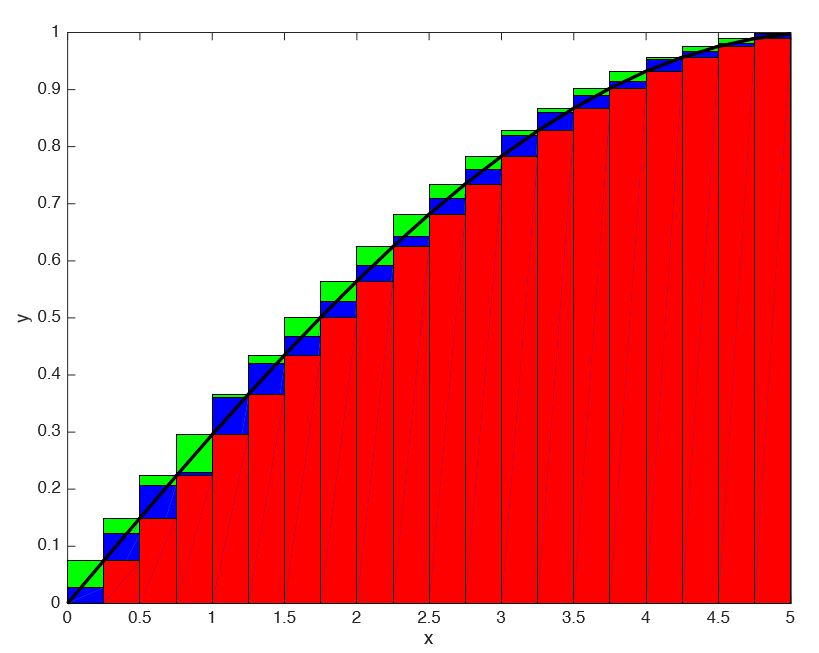
\includegraphics[width=0.5\textwidth]{AC1.jpg}
\caption{Riemann Sum Diagram on an arbitrary graph}
\end{figure}

\begin{itemize}
\item
$f(x)$ is the \textcolor{red}{integrand}, $a$ the \textcolor{red}{lower limit}, $b$ the \textcolor{red}{upper limit}. 
\item
Each finite sum is called a \textcolor{red}{Riemann} or partial sum.
\item
The definite integral can be interpreted as the ``area under the curve'' $y=f(x)$ from $a$ to $b$ ($0$ to $5$ in the example above)
\end{itemize}
\textbf{Claim:}
$$
\int_a^b f(x) dx=\textcolor{green}{ \lim_{n \to \infty} \sum_{j=1}^{n} f(x_j) \Delta x} =  \textcolor{red}{ \lim_{n \to \infty} \sum_{j=0}^{n-1} f(x_j) \Delta x}\,.
$$
\begin{proof}
Recall from Calculus (ECM1901) that a sequence $\left\{ s_n \right\}$ has a limit $s$, i.e.
$$
s_n \rightarrow s \mbox{ as } n \rightarrow \infty\,,
$$
if for each $\epsilon > 0$ we can find
$N$ so that if $n \geq N$, then $|s_n - s| < \epsilon$. 


We will use notion  of convergent sequence with $s = \int_a^b f(x) dx$ and 
$$
\mbox{either    } s_n = \sum_{j=0}^{n-1} f(x_j) \Delta x \mbox{    or    } s_n = \sum_{j=1}^{n} f(x_j) \Delta x\,.
$$
Assume that
$$
\int_a^b f(x) dx =  \textcolor{red}{\lim_{n \to \infty} \sum_{j=0}^{n-1} f(x_j) \Delta x}\,.
$$
Now
{\small 
$$
\int_a^b f(x) dx -  \sum_{j=1}^{n} f(x_j) \Delta x = \int_a^b f(x) dx -  \sum_{j=0}^{n-1} f(x_j) \Delta x - (\Delta x) \times \left( f(b) - f(a) \right).
$$
}
Chose $\epsilon > 0$. By definition, there exists $N_1$ so that if $n \geq N_1$, then
\begin{equation}
\left|\int_a^b f(x) dx -  \sum_{j=0}^{n-1} f(x_j) \Delta x \right| < \frac{\epsilon}{2}\,.
\end{equation}
We can also choose $N_2$ (bigger than $N_1$ if needed) so that if $n \geq N_2$, then 
\begin{equation}
(\Delta x) \times \left( f(b) - f(a) \right) = \frac{b-a}{n} \times \left( f(b) - f(a) \right) < \frac{\epsilon}{2}\,.
\end{equation}
If now follows that for the given given $\epsilon > 0$, we can, using (1) and (2), find $N$ so that if $n \geq N$ then
$$
\left|\int_a^b f(x) dx -  \sum_{j=1}^{n} f(x_j) \Delta x \right| < \epsilon \mbox{  and  } \textcolor{green}{ \lim_{n \to \infty} \sum_{j=1}^{n} f(x_j) \Delta x} = \int_a^b f(x) dx\,.
$$
\end{proof}
\hrulefill

\textbf{Example I1.} Using the definition to evaluate a definite integral.

Let 
$$
f(x) = x^3 - 6x, a=0, b=3
$$
Then we know (do we?) that
$$
\begin{array}{ll}
I:= \displaystyle\int_0^3 (x^3- 6x) dx & =\left[ x^4/4-3x^2 \right]_0^3\\
& =81/4-27=(81-108)/4= -27/4\,.
\end{array}
$$
Now let us compute $I$ by Riemann sums. First we set up the partition of the interval $[0, 3]$ so that
$$
\Delta x= (b-a)/n= 3/n, \; x_0=0, x_1=3/n, x_2=6/n, ..., x_j=3j/n,
$$
Then from first principles:
$$
I = \lim_{n \to \infty} \sum_{j=1}^{n } f(x_j) \Delta x =  \lim_{n \to \infty}\sum_{n=1}^{n} f(\frac{3j}{n})
  \frac{3}{n}  
$$
$$
\begin{array}{ll}
I = & \displaystyle\lim_{n \to \infty}  \sum_{j=1}^{n} \left[ \left(\frac{3j}{n}\right)^3-6 \left(\frac{3j}{n}\right) \right] \frac{3}{n}  \\
\\
= & \displaystyle \lim_{n \to \infty} \sum_{j=1}^{n} \left[ \frac{27j^3}{n^3} -\frac{18j}{n} \right] \frac{3}{n} \\
\\
= & \displaystyle \lim_{n \to \infty} \left[ \frac{81}{n^4}  \sum_{j=1}^{n} j^3 - \frac{54}{n^2} \sum_{j=1}^{n} j \right].
\end{array}
$$
But
$$
\sum_{j=1}^{n} \; j= \frac{n(n+1)}{2}, \;\; 
\sum_{j=1}^{n} \; j^2= \frac{n(n+1)(2n+1)}{6},
\sum_{j=1}^{n}j^3= \left[ \frac{n(n+1)}{2} \right]^2.
$$
Hence
\begin{eqnarray}
 I & = & \lim_{n \to \infty} \left[ \frac{81}{n^4}\left(
\frac{n(n+1)}{2} \right)^2   - \frac{54}{n^2} \frac{n(n+1)}{2}
\right]  \nonumber \\
  & = & \lim_{n \to \infty} \left[ \frac{81}{4}\left( 1+
\frac{1}{n} \right)^2   - 27 \left( 1+ \frac{1}{n} \right) \right]
 \nonumber \\
 & = &  \frac{81}{4}-27=  - \frac{27}{4} \nonumber
\end{eqnarray}
\hrulefill

Note that we do not need to use a partition 
$$
{\cal P}_n: x_0=a, x_1= a + \Delta x, \ldots, x_{n-1}, x_n = a+ n \Delta x= b
$$ 
with uniform separation 
$$
\Delta x = \frac{b-a}{n}\,,
$$
and any partition ${\cal P}_n: x_0^n=a, x_1^n, \ldots, x_{n-1}^n, x_n^n = b$ of $[a, b]$ would be allowed.

What is crucial is that the partition ${\cal P}_n$ becomes finer as $n \rightarrow \infty$\,.

In this case, we can alternatively say that
$$
\int_a^b f(x) dx = \lim_{n \rightarrow \infty} \sum_{i=1}^n f(x_i^n) (x_{i}^n-x_{i-1}^n)
$$
where in the limit as $n \rightarrow \infty$ we assume a partition ${\cal P}_n$ that gets finer with increasing $n$.
\begin{itemize}
\item
Note that in approximating the integral from $a$ to $b$ by a finite sum obtained from (increasingly finer) partitions of $[a, b]$,
continuity of the function $f(x)$ plays a crucial role. 
\item
If we drop continuity of $f(x)$ then the process collapses and bizarre things can happen.
\item
By way of illustration of how bizarre it gets --- consider the function
$$
f(x) = \left\{ \begin{array}{ll} 1 & \mbox{if } x \mbox{ is rational,}\\ 0 & \mbox{if } x \mbox{ is irrational.} \end{array} \right.
$$
This function is not continuous at any $x \in [0, 1]$. Convince your self that for any given $A \in (0, 1)$, there exists a sequence of partitions 
$$
{\cal P}_n : 0=x_0^n, x_1^n, \ldots, x_{n-1}^n, x_n^n = 1, \qquad n = 1, 2, 3, \ldots
$$
so that
$$
\lim_{n \rightarrow \infty} \sum_{k=1}^{n} f(x_{k-1}^n) \left( x_k^n - x_{k-1} ^n\right) = A\,.
$$
\end{itemize}
\subsection{Properties  of the definite integral}
\vspace{-.3cm}

\begin{eqnarray}
& (1) & \int_a^b f(x) dx = -\int_b^a f(x) dx   \nonumber \\
& (2) &\int_a^a f(x) dx = 0    \nonumber \\
& (3) &\int_a^b [f(x)+g(x)] dx = \int_a^b f(x) dx + \int_a^b g(x)
dx
\nonumber \\
& (4) & \int_a^b f(x) dx = \int_a^c f(x) dx + \int_c^b f(x) dx, \;
a<c<b    \nonumber \\
& (5) & \int_a^b f(x) dx \ge 0,\; \mbox{ if
} \; f(x) >0, \; a \leq x \leq b
 \nonumber \\
 & (6) & \int_{-a}^a f(x) dx =2 \int_{0}^a f(x) dx ,\; \mbox{ if
} \; f(x)= f(-x)
 \nonumber \\
& (7) & \int_{-a}^a f(x) dx = 0 ,\; \mbox{ if } \; f(x)= -f(x)
 \nonumber
 \end{eqnarray}
\subsection{Some proofs}
We can, without loss of generality, work with \textcolor{green}{right-hand} Riemann sum and partitions
$$
a=x_0, \ldots, x_n = b, \mbox{    and   } \Delta = \frac{b-a}{n}
$$
(1) \textbf{Claim:}
$$
\int_a^b f(x) dx = -\int_b^a f(x) dx\,. \qquad
$$
\begin{proof}
{\small 
$$
\int_a^b f(x) dx = \lim_{n \rightarrow \infty} \frac{b-a}{n} \sum_1^n f(x_i) = - \lim_{n \rightarrow \infty} \frac{a-b}{n} \sum_n^1 f(x_i) = -\int_b^a f(x) dx\,.
$$
}
\end{proof}
(3) \textbf{Claim:}
$$ \int_a^b [f(x)+g(x)] dx = \int_a^b f(x) dx + \int_a^b g(x)
dx $$
\begin{proof}
Using the algebra of limits we have that:
{\small 
$$
\begin{array}{ll}
 \displaystyle\int_a^b [f(x)+g(x)] dx & = \lim_{n \rightarrow \infty} \frac{b-a}{n} \sum_1^n \left(f(x_i)+g(x_i) \right) \\
\\
& =   \displaystyle\lim_{n \rightarrow \infty} \frac{b-a}{n} \sum_1^n f(x_i)+ \lim_{n \rightarrow \infty} \frac{b-a}{n} \sum_1^n g(x_i) \\
\\
& =  \displaystyle\int_a^b f(x) dx + \int_a^b g(x) dx
\end{array}
$$
}
\end{proof}
(4) \textbf{Claim:}
$$ \int_a^b f(x) dx = \int_a^c f(x) dx + \int_c^b f(x) dx, \;
a<c<b $$
\begin{proof}
If 
$${\cal P}_n: x_0 = a, x_1, \ldots, x_n = c
$$ 
is a partition of $[a, c]$ and 
$$
{\cal Q}_n: z_0 = c, z_1, \ldots, z_n = b
$$ 
is a partition of $[c, b]$ then
$$
\begin{array}{ll}
{\cal R}_n & = {\cal P}_n \cup {\cal Q}_n\\
\\
& : y_0 = x_0 = a, \ldots, y_n = x_n = c, y_{n+1} = z_1, \ldots, y_{2n} = b
\end{array}
$$
is a partition of $[a, b]$. Then
$$
\begin{array}{ll}
& \displaystyle \int_a^c f(x) dx + \int_c^b f(x) dx \\
\\
& =  \displaystyle\lim_{n \rightarrow \infty} \sum_1^n f(x_i) (x_i-x_{i-1})+ \lim_{n \rightarrow \infty} \sum_1^n f(z_i) (z_i-z_{i-1})\\
\\
& = \displaystyle \lim_{n \rightarrow \infty} \sum_1^{2n} f(y_i) (y_i-y_{i-1}) = \int_a^b f(x) dx\,.
\end{array}
$$
\end{proof}
\section{The Fundamental Theorem of Calculus}
\begin{theorem}[FTC]
Suppose $f$ is continuous on $[a,b]$
\begin{eqnarray}
& (1) & \mbox{ If } g(x)=\int_a^x f(t) \; dt, \; \mbox{ then } \;
\frac{d g}{d x}= f(x); \;\; \mbox{ or  } \nonumber \\ 
& & \frac{d }{d x} \int_a^x f(t) dt =f(x)
\nonumber \\
& (2) &\int_a^a f(x) dx = F(b)-F(a),    \nonumber
\end{eqnarray}
where $F$ is any anti-derivative of $f$, i.e., $d F/dx=f$. Also
\begin{eqnarray}
& & \frac{d }{d x} \int_{a(x)}^{b(x)} f(t) dt = \frac{d }{d x} \left(F(b(x))-F(a(x))\right) \nonumber\\ 
&& = F'(b(x))b'(x) - F'(a(x))a'(x) = f(b(x))b'(x)-f(a(x)) a'(x).    \nonumber
\end{eqnarray}
\end{theorem}
{\large \bf The Total Change Theorem:}
\begin{theorem}[Total Change Theorem]
\begin{eqnarray}
& &\int_a^b F'(x) dx = F(b)-F(a).    \nonumber
\end{eqnarray}
Some examples of differentiating an integral:
$$
\begin{array}{ll}
 \displaystyle\frac{d}{dx} \int_1^{x^3} y^2 dy 
& = (x^3)^2(3 x^2)- (1)^2(0) \\
\\
& = 3 x^8
\end{array}
$$
$$
\begin{array}{ll}
 \displaystyle\frac{d}{dx} \int_{-\cos x}^{\sin x} y^3 dy & = (\sin x)^3(\cos x) - (-\cos x)^3 (+\sin x) \\
\\
& = (\sin x \cos x)(\sin^2 x + \cos^2 x) =  \sin x \cos x\,.
\end{array}
$$
\end{theorem}
\subsection{Gappy Proof of FTC}
\begin{proof}
We assume that
$$
f(x) = F'(x) \mbox{ for some function } F(x)
$$
We know, from the Mean Value Theorem (for derivatives) that for any $\alpha$ and $\beta$, $\beta > \alpha$:
$$
\frac{F(\beta) - F(\alpha)}{\beta - \alpha} = F'(c), \mbox{ some } c \in [\alpha, \beta]
$$
Then, from the Riemann definition of the integral via partial sums:
$$
\int_a^b f(x) dx= \lim_{n \to \infty} \sum_{j=1}^{n} f(\textcolor{red}{c_j}) \Delta x =  \lim_{n \to \infty} \sum_{j=1}^{n} F'(\textcolor{red}{c_j}) \Delta x, \;\;  \textcolor{blue}{x_{j-1} \leq c_j \leq x_{j}}\,.
$$
Choosing \textcolor{red}{$c_j$} according to the MVT with \textcolor{red}{$\alpha = x_{j-1}$} and \textcolor{red}{$\beta = x_j = x_{j-1} + \Delta x$} gives:
{\small 
$$
\int_a^b f(x) dx = \lim_{n \to \infty} \overbrace{\sum_{j=1}^{n} \frac{F(x_j) - F(x_{j-1})}{\Delta x} \Delta x}^{\mbox{\textcolor{red}{telescopic sum}}}= F(b) - F(a)
$$
}
\end{proof}
\newpage
\subsection{The Fundamental Theorem and Integration - an example}
\textbf{Example I2.} Evaluate the definite integral
$$
I=\int_0^3 f(x)  dx = \int_0^3 (x^3- 6x) dx,
$$
First observe that:
$$
\frac{d}{d x} \left( \frac{1}{4}x^4-3 x^2 \right)=x^3- 6x=f(x).
$$
So an anti-derivative of $f(x)$ is $F(x)=\frac{1}{4}x^4-3 x^2$.  

The fundamental Theorem of Calculus then gives
$$
\begin{array}{ll}
I & = \displaystyle\int_0^3 f(x)  dx =F(3) -F(0) \\ 
\\ & = \frac{1}{4} 3^4-3\cdot3^2 =\frac{3}{4} 27- 27= -\frac{27}{4}
\end{array}
$$
\section{Indefinite integrals}  
An anti-derivative of $f$, $ \int f(x) dx =F(x)$ is called an indefinite integral, i.e.,
\begin{eqnarray}
&  &\int  f(x) d x =F(x) \;\;  \; \mbox{ means } \; \frac{d
F(x)}{d x}= f(x).    \nonumber
\end{eqnarray}
Integration is the inverse of differentiation.

\begin{itemize}
\item
A definite integral is a number
\item
an indefinite integral is a function.
\end{itemize}


\section{Methods of integration} 
\subsection{Basic integrals obtained from differentiating well known functions}

\begin{eqnarray}
&(1)& \frac{d }{d x} \left( \sin x \right) = \cos x  \;   \to   \;
\int \cos x  = \sin x +C
\nonumber \\
&(2)& \frac{d }{d x} \left( \cos x \right) = -\sin x  \;   \to \;
\int \sin x  = -\cos x +C    \nonumber \\
&(3)& \frac{d }{d x} \left( \tan x \right) = \frac{1}{\cos^2 x}
\;   \to \;
\int \frac{1}{\cos^2 x} dx   = \tan x +C  \nonumber
\\
&&(\sec x=1/\cos x)    \nonumber \\
&(4)& \frac{d }{d x} \left( \cot x \right) = - \frac{1}{\sin^2 x}
\;   \to \;
\int \frac{1}{\sin^2 x}  = - \cot x +C  \nonumber
\\
&& (\mathrm{cosec}\, x=1/\sin x)    \nonumber 
\end{eqnarray}
\begin{eqnarray}
&(5)& \frac{d }{d x} \left( \frac{x^{n+1}}{n+1} \right) =  x^n \;
\to \;
\int x^n \; dx =  \frac{x^{n+1}}{n+1}  +C  \; \;     \nonumber \\
&(6)& \frac{d }{d x} \left( \sin^{-1} x  \right) =
\frac{1}{\sqrt{1-x^2} } \; \to \;
\int \frac{d x}{\sqrt{1-x^2} }  = \sin^{-1} x +C     \nonumber \\
&(7)& \frac{d }{d x} \left( \tan^{-1} x  \right) = \frac{1}{1+x^2}
\; \to \;
\int \frac{d x}{1+x^2 }  = \tan^{-1} x +C     \nonumber \\
&(8)& \frac{d }{d x} \left( e^x \right) = e^x  \;   \to   \; \int
e^x  = e^x +C\nonumber
\nonumber \\
&(9)& \frac{d }{d x} \left( \ln |x|  \right) =  \frac{1 }{x} \;
\to \; \int \left( \frac{1 }{x} \right) d x  = \ln |x| +C
\nonumber \\
&(10)& \frac{d }{d x} \left( a^x  \right) = a^x \ln a \; \to \;
\int \left( a^x \right) d x  = \frac{a^x}{\ln a}  +C \nonumber \\
&(11)& \frac{d }{d x} \left( \sinh x  \right) =  \cosh x \; \to \;
\int \left( \cosh x \right) d x  = \sinh x  +C, \nonumber
\\
 && \sinh x=(e^x-e^{-x})/2 \nonumber \\
 &(12)& \frac{d }{d x} \left( \cosh x \right) =
\sinh x \; \to \; \int \left( \sinh x \right) d x  = \cosh x  +C, \nonumber
\\
&& \cosh x=(e^x+e^{-x})/2 \nonumber
\end{eqnarray}


\subsection{Integration by substitution}

If $ u=u(x)$ is a differentiable function and $f$ is continuous, then
$$
\int f( u(x) ) \left( u'(x) dx \right) = \int f( u ) du \quad \mbox{indefinite integral}
$$
$$
\int_a^b f( u(x) ) \left( u'(x) dx \right) = \int_{u(a)}^{u(b)} f(u ) du \quad \mbox{definite integral}.
$$
Here {\bf  $d u$ acts as if it is a differential.}
 $$
 d u= u' d x, \;\;  d (c+x)=dx; \;\; d (x^2)=2x dx, \;\; d (\sin x)= \cos x d x, ...,
 $$
\hrulefill

 \textbf{Example I3.} Evaluate  the indefinite integral
$$
I=\int 2 x \sqrt{1+x^2}  dx.
$$
Introduce $u=1+x^2$, then $d u =u'(x) d x=2x \; dx$ and we can write
$$
I=\int  \sqrt{(1+x^2)} (2x dx)= \int  {u}^{1/2} du=\frac{2}{3}
u^{3/2}+C= \frac{2}{3} (1+x^2)^{3/2}+C .
$$

\newpage
\textcolor{red}{\textbf{Exercise I4.}} Evaluate  the indefinite integral
$$
I=\int  x^3 \cos (2+x^4)  dx.
$$

\textcolor{white}{then $d u =u'(x) d x=4x^3 \; dx$ and we can write
{\small
$$
I=\int  \cos(2+x^4) \frac{1}{4} (4x^3 dx) = \int \frac{1}{4} \cos
u du=\frac{1}{4} \sin u +C = \frac{1}{4} \sin (2+x^4) +C.
$$
}
}
\vspace*{100px}

\section{Methods of integration} 
\subsection{Integrals of trigonometric and hyperbolic functions}

Here we make extensive use of double-angle formulas,  addition/subtraction formulas
and trigonometric substitution:
$$
\sin (x\pm y) =\sin x \cos y \pm \cos x \sin y, \;\; \cos (x\pm y) =\cos x \cos y \mp \sin x \sin y
$$
$$
\cos 2x =\cos^2 x -\sin^2 x = 2 \cos^2 x - 1 = 1 - 2 \sin^2 x
$$
$$
\sin 2x =2 \sin x \cos x
$$
$$
\sin x \cos y =\frac{1}{2} \left[ \sin(x-y)+ \sin(x+y) \right]
$$
$$
\sin x \sin y =\frac{1}{2} \left[ \cos(x-y) - \cos(x+y) \right]
$$
$$
\cos x \cos y =\frac{1}{2} \left[ \cos(x-y)+ \cos(x+y) \right]
$$
$$
\cosh^2x - \sinh^2 x =1.
$$
\hrulefill

\textbf{Example I5.} Evaluate  the definite integral
\begin{eqnarray}
& I & =\int_0^{\pi} \sin^2 x  dx  \nonumber \\
&   & =\int_0^{\pi} \frac{1}{2} \left( 1 - \cos 2x \right)  dx  = \frac{1}{2} \left[ x - \frac{1}{2}\sin 2x \right]_0^{\pi}
= \frac{\pi}{2}   \nonumber
\end{eqnarray}
\textbf{Example I6.}
Evaluate the indefinite integral
\begin{eqnarray}
& I & =\int  (\sin^2 x)^2  dx  = \int \frac{1}{4} \left( 1 - \cos 2x \right)^2  dx  \nonumber \\
&   & =\int \frac{1}{4} \left( 1 - 2\cos 2x +\cos^2 2x
\right)  dx
\nonumber \\
&   & =\int \frac{1}{4} \left[  1 - 2\cos 2x +
\frac{1}{2} \left( 1 - \cos 4x \right) \right]  dx  \nonumber \\
&   & = \frac{1}{4} \left[ \frac{3}{2} x -\sin 2x + \frac{1}{8}
\sin 4x \right]  +C    \nonumber
\end{eqnarray}


\textcolor{red}{\textbf{Exercise I7.}}
Evaluate  the indefinite integral
\begin{eqnarray}
& I & =\int  (\sin4x \cos 5x )  dx  \textcolor{white}{=\int \frac{1}{2} \left[ \sin (-x) +\sin 9x \right]  dx  }\nonumber \\
&   & \textcolor{white}{=\frac{1}{2} \left( \cos x  - \frac{1}{9} \cos 9x \right) +C}
\nonumber
\end{eqnarray}
\vspace{100px}

\textbf{Example I8.}
Evaluate  the indefinite integral
\begin{eqnarray}
& I & =\int  \frac{\sqrt{9-x^2}}{x^2}  dx \; \;
[x=3\sin \theta, \;\; -\frac{\pi}{2} \leq \theta \leq \frac{\pi}{2}] \nonumber \\
&   & =\int  \frac{\sqrt{9-(3\sin \theta)^2} }{(3\sin \theta)^2}  d (3\sin \theta)  \nonumber \\
&   & = \int  \frac{3\cos \theta  }{9\sin^2 \theta } \; (3\cos
\theta) = \int  \frac{\cos^2  \theta  }{\sin^2 \theta } d \theta  \nonumber \\
& & =  \int  \frac{1- \sin^2  \theta  }{\sin^2 \theta } d \theta  = \int \left(  \frac{1 }{\sin^2 \theta } -1 \right) d \theta  \nonumber =  -\cot \theta -\theta +C  \nonumber
\end{eqnarray}


\textbf{Exercise I7.}
Evaluate  the indefinite integral
\begin{eqnarray}
& I & =\int  (\sin4x \cos 5x )  dx  =\textcolor{white}{\int \frac{1}{2} \left[ \sin (-x) +\sin 9x \right]  dx  }\nonumber \\
&   & \textcolor{white}{=\frac{1}{2} \left( \cos x  - \frac{1}{9} \cos 9x \right) +C}
\nonumber
\end{eqnarray}
\vspace{100px}

\textbf{Exercise I8.}
Evaluate  the indefinite integral
\begin{eqnarray}
& I & =\int  \frac{\sqrt{9-x^2}}{x^2}  dx \; \;
\textcolor{white}{[x=3\sin \theta, \;\; -\frac{\pi}{2} \leq \theta \leq \frac{\pi}{2}] \nonumber} \\
&   & \textcolor{white}{ =\int  \frac{\sqrt{9-(3\sin \theta)^2} }{(3\sin \theta)^2}  d (3\sin \theta)  \nonumber} \\
&   &  \textcolor{white}{= \int  \frac{3\cos \theta  }{9\sin^2 \theta } \; (3\cos
\theta) = \int  \frac{\cos^2  \theta  }{\sin^2 \theta } d \theta  \nonumber} \\
& & \textcolor{white}{=  \int  \frac{1- \sin^2  \theta  }{\sin^2 \theta } d \theta  = \int \left(  \frac{1 }{\sin^2 \theta } -1 \right) d \theta  \nonumber =  -\cot \theta -\theta +C  \nonumber}
\end{eqnarray}
\vspace{100px}

\textcolor{red}{\textbf{Exercise I9.}}
Evaluate the indefinite integral
\begin{eqnarray}
& I & =\int  \frac{d x} {\sqrt{x^2-a^2} }  \; \;
[x=a \cosh t]  \nonumber \\
&   & \textcolor{white}{=\int  \frac{ d(a\cosh t)} { \sqrt{a^2(\cosh^2-1)} }  } \nonumber \\
&   & \textcolor{white}{= \int dt = t +C = \cosh^{-1} \frac{x  }{a } +C}  \nonumber
\end{eqnarray}
\vspace{100px}

%
%\textbf{Example I9.}
%Evaluate the indefinite integral
%\begin{eqnarray}
%& I & =\int  \frac{d x} {\sqrt{x^2-a^2} }  \; \;
%[x=a \cosh t, \;\; \cosh^2 t- \sinh^2 t=1]  \nonumber \\
%&   & \textcolor{red}{=\int  \frac{ d(a\cosh t)} { \sqrt{a^2(\cosh^2-1)} }  } \nonumber \\
%&   & \textcolor{red}{= \int dt = t +C = \cosh^{-1} \frac{x  }{a } +C}  \nonumber
%\end{eqnarray}
%

\subsection{Integrals of rational functions using partial fractions}

Let 
$$
d(x) = (x-a_1) (x-a_2) \ldots (x-a_{n-1})(x-a_n), \qquad a_i \mbox{ distinct}
$$
If $n(x)$ is a polynomial of degree $n$ or less, then
$$
\frac{n(x)}{d(x)} = \sum_{i=1}^n \left( \frac{n(a_i)}{\prod_{j \neq i} (x-a_j)} \right) \frac{1}{x-a_i}
$$
Now we know that
$$
\frac{d}{dx} \ln (x-a) = \frac{1}{x-a}
$$
By using this fact repeatedly, we can then integrate any rational function of the form
$$
\frac{n(x)}{d(x)}
$$
above - but the answer depends on the details (because $\ln z$ is only defined for positive $z$).\\
\hrulefill

\textbf{Example I10.} Evaluate  the indefinite integral
\begin{eqnarray}
& I & =\int  \frac{2x^2 -x + 4} { x(x^2+4) } dx \; \;  \nonumber\\
& &  \left[ \frac{2x^2 -x + 4} { x(x^2+4)}=\frac{A} { x}+
\frac{Bx+C} {(x^2+4)},
A=1, B=1, C=-1 \right]   \nonumber \\
& I  & =\int \left[ \frac{1} {x}  + \frac{x-1} {x^2 +4 } \right]  \nonumber \\
&   & =\int  \frac{dx} {x} +  \int  \frac{x} {x^2 +4 } dx -\int  \frac{1} {x^2 +4 } dx  \nonumber \\
&   & = \ln |x| +\frac{1}{2} \ln (x^2 +4) - \frac{1}{2} \tan^{-1}(x/2)+C  \nonumber
\end{eqnarray}


\textcolor{red}{\textbf{Exercise I11.}} Evaluate the indefinite integral (the
degree of the numerator is not less than the degree of the
denominator)
\begin{eqnarray}
& I & =\int  \frac{4x^2 -3x + 2} { 4x^2 -4x +3 } dx \; \;  \nonumber\\
& &  \textcolor{white}{\displaystyle \frac{4x^2 -3x + 2} { 4x^2 -4x +3 }=1+\frac{x-1} { 4x^2 -4x +3 }; 4x^2 -4x +3=( 2x -1)^2 +2}   \nonumber \\
&   & \textcolor{white}{\int \left[ 1+ \frac{x-1} {(2x-1)^2+2 } \right]dx } \nonumber \\
&    & \textcolor{white}{= x+ \int \left[ \frac{ (1/2)(2x-1)-(1/2) } {(2x-1)^2+2 } \right] (1/2) d(2x-1)  } \nonumber \\
&    & \textcolor{white}{=x+\int  \left(\frac{1}{4}  \frac{(2x-1)} {(2x-1)^2+2 } - \frac{1}{4}  \frac{1} {(2x-1)^2+2 } \right)  d(2x-1)}
  \nonumber \\
& & \textcolor{white}{=x+  \frac{1}{8}  \ln[(2x-1)^2+2] -  \frac{1}{4 \sqrt{2}}
\tan^{-1} \frac{2x-1}{ \sqrt{2}} +C  } \nonumber
\end{eqnarray}

%
%\textbf{Example I11.} Evaluate  the indefinite integral (the
%degree of the numerator is not less than the degree of the
%denominator)
%\begin{eqnarray}
%& I & =\int  \frac{4x^2 -3x + 2} { 4x^2 -4x +3 } dx \; \;  \nonumber\\
%& &  {\small \frac{4x^2 -3x + 2} { 4x^2 -4x +3 }=1+\frac{x-1} { 4x^2 -4x +3 }; 4x^2 -4x +3=( 2x -1)^2 +2}   \nonumber \\
%& I  & =\textcolor{red}{\int \left[ 1+ \frac{x-1} {(2x-1)^2+2 } \right]dx } \nonumber \\
%&    & \textcolor{red}{= x+ \int \left[ \frac{ (1/2)(2x-1)-(1/2) } {(2x-1)^2+2 } \right] (1/2) d(2x-1)  } \nonumber \\
%&    & \textcolor{red}{=x+\int  \left(\frac{1}{4}  \frac{(2x-1)} {(2x-1)^2+2 } - \frac{1}{4}  \frac{1} {(2x-1)^2+2 } \right)  d(2x-1)}
%  \nonumber \\
%& & \textcolor{red}{=x+  \frac{1}{8}  \ln[(2x-1)^2+2] -  \frac{1}{4 \sqrt{2}}
%\tan^{-1} \frac{2x-1}{ \sqrt{2}} +C  } \nonumber
%\end{eqnarray}
%

\subsection{Integration by parts}

According to the product rule from Calculus: If $u(x)$ and $v(x)$ are
differentiable functions, then
{\small 
$$
\frac{d (u(x)v(x))}{dx}=u(x) v'(x)+v(x) u'(x).
$$
}
From the Fundamental Theorem of Calculus it follows that
$$
\int \frac{d}{dx} \left( u(x)v(x) \right) dx = u(x)v(x)= \int \left[u(x) v'(x)+v(x) u'(x)\right] dx,
$$
or
{\small 
$$
u(x)v(x)=  \int u(x) v'(x) dx + \int  v(x) u'(x) dx.
$$
}
Rearranging gives:
$$
\int u(x) v'(x) dx= u(x)v(x) - \int  v(x) u'(x) dx.
$$
So given
$$
\int f(x) g(x) dx
$$
we look to set \textcolor{red}{$f(x) = u(x)$} and \textcolor{blue}{$g(x) = v'(x)$}.
%The formula for integration by parts is
%$$
%\int u \; dv = uv - \int  v \; d u.
%$$



\textbf{Example I12.} Evaluate  the indefinite integral
$$
I=\int \ln x \; dx = \int \ln x \,\, 1 \,dx,
$$
where we take
$$
u=\ln x, \;\; v=x \implies v'(x) = 1
$$
\begin{eqnarray}
& I & = uv - \int  v u' dx = x \ln x - \int x \frac{1}{x} dx  \; \;  \nonumber\\
&   & =  x \ln x - \int  \,1 \, d x \; \; \nonumber\\
&   & =  x \ln x - x +C \; \; \nonumber
  \nonumber
\end{eqnarray}


\textbf{Example I13.} Evaluate the indefinite integral
$$
I=\int x^2 e^x \; dx,
$$
where we take
$$
u=x^2, \;\; v=e^x, \implies v'(x)= e^x.
$$
\begin{eqnarray}
& I & = uv - \int  v u' dx = x^2 e^x - \int e^x  2x \, dx  =   x^2 e^x - 2 \int e^x \, x \, d x  \nonumber
\end{eqnarray}
We need to use integration by parts again by taking
$$
u=x, \;\; v=e^x \implies v'(x) = e^x
$$
\begin{eqnarray}
& I & = x^2 e^x -  \left( 2 \int x  e^x \, dx \right)  =   x^2 e^x - \left( 2 x e^x - 2 \int e^x \,d x \right)
\nonumber\\
 &   & =   x^2 e^x - \left( 2 x e^x - 2 e^x  +C
\right) \nonumber
\end{eqnarray}


\textcolor{red}{\textbf{Class Example I14.}} Evaluate  the indefinite integral
$$
I=\int e^x  \sin x \;   dx,
$$
where we take $u=e^x, \;\; v=-\cos x, \;\;  v'=\sin x $
\textcolor{white}{
\begin{eqnarray}
& I & = uv - \int  v \, u' dx = - e^x \cos x  + \int \cos x e^x  d x  \; \;  \nonumber\\
&   & = - e^x \cos x  + \left( \int e^x (\sin x)' dx  \right)
\nonumber\\
&   & = - e^x \cos x  + \left( \sin x  e^x -  \int  \sin  x e^x\, dx
\right) \nonumber \\
&& = - e^x \cos x  + \sin x  e^x - I \nonumber
\nonumber
\end{eqnarray}
Solving for $I$:
\begin{eqnarray}
& I & =  (- e^x \cos x  +  \sin x  e^x)/2 + C \nonumber
\end{eqnarray}
}

%
%\textcolor{red}{\textbf{Example I14.}} Evaluate  the indefinite integral
%$$
%I=\int e^x  \sin x \;   dx,
%$$
%where we take $u=e^x, \;\; v=-\cos x, \;\;  dv= d (-\cos x)=\sin x \; dx $
%\textcolor{red}{
%\begin{eqnarray}
%& I & = uv - \int  v \; d u= - e^x \cos x  + \int \cos x e^x  d x  \; \;  \nonumber\\
%&   & = - e^x \cos x  + \left( \int e^x d \sin x \right)
%\nonumber\\
%&   & = - e^x \cos x  + \left( \sin x  e^x -  \int  \sin  x d e^x
%\right) \nonumber \\
%&& = - e^x \cos x  + \sin x  e^x - I \nonumber
%\nonumber
%\end{eqnarray}
%Solving for $I$:
%\begin{eqnarray}
%& I & =  (- e^x \cos x  +  \sin x  e^x)/2 + C \nonumber
%\end{eqnarray}
%}
%

\section{Improper Integrals:} 

The integral is called an improper integral when
\begin{itemize}
\item
the interval is infinite or
\item
$f(x)$ has an infinite discontinuity in $[a,b]$.
\end{itemize}

\subsection{Improper Integrals - Type I}

If $\int_a^t f(x) dx $ exists for every number $t \geq a$,
then
$$
\int_a^{\infty} f(x) dx = \lim_{t \to \infty} \int_a^{t} f(x) dx,
$$
provided this limit exists (convergent).

\hrulefill

\textbf{Example I15.} Evaluate  the improper integral
$$
I=\int_{-\infty}^0 x e^x \;   dx
$$
i.e.,
\begin{eqnarray}
& I & =\int_{-\infty}^0 x e^x \;   dx=\lim_{t \to -\infty} \int_{t}^0 x e^x \;  d x  \; \;  \nonumber\\
&   & = \lim_{t \to -\infty}  \left[ \int_{t}^0 x  d e^x \right]= \lim_{t \to -\infty}  \left[ xe^x - \int_{t}^0  e^x \; dx
\right]\nonumber\\
&   & = \lim_{t \to -\infty}  \left[ xe^x -   e^x \right]_t^0 = \lim_{t \to -\infty}  \left[ te^t -  1 + e^t \right]= -1
\nonumber
\end{eqnarray}



\textbf{Example I16.} Evaluate  the improper integral
$$
I=\int_0^{\infty} \frac{1}{1+x^2} \;   dx
$$
i.e.,
\vspace{-1cm}

\begin{eqnarray}
& I & =\int_{0}^{\infty} \frac{1}{1+x^2} \;   dx=
\lim_{t \to \infty} \int_{0}^t \frac{1}{1+x^2}\; \;  d x  \; \;  \nonumber\\
&   & = \lim_{t \to \infty}  \left[ \tan^{-1} x \right]_0^t \nonumber\\
&   & = \lim_{t \to \infty}  \left[ \tan^{-1} t - \tan^{-1}0\right]\nonumber\\
&   & = \pi/2  \nonumber
\end{eqnarray}


\subsection{Improper Integrals - Type II}

If $f(x)$  is continuous on $(a,b]$, and is discontinuous
at \textcolor{red}{$b$}, then
$$
\int_a^{b} f(x) dx = \lim_{t \to a^+} \int_t^{b} f(x) dx,
$$
provided this limit exists (convergent).

\hrulefill

\textbf{Example I17.}  Evaluate  the improper integral
$$
I=\int_2^{5} \frac{1}{\sqrt{x-2} } \;   dx
$$
i.e.,
\begin{eqnarray}
& I & =\int_{2}^{5} \frac{1}{\sqrt{x-2}} \;   dx=
\lim_{t \to 2^+} \int_{t}^5 \frac{1}{\sqrt{x-2}}\; \;  d x  \; \;  \nonumber\\
& & = \lim_{t \to 2^+} \int_{t}^5 \frac{d (x-2)}{\sqrt{x-2}} \; \;  \nonumber\\
& & = \lim_{t \to 2^+} \left[ 2  (x-2)^{1/2} \right]_t^5 = \lim_{t \to 2^+} \left[ 2 \sqrt{3}-2 \sqrt{t-2} \right] = 2 \sqrt{3} \; \; \nonumber
\end{eqnarray}


\textcolor{red}{\textbf{Exercise I18.}} Evaluate  the improper integral
$$
I=\int_0^{1} \ln x  \;   dx
$$
\begin{eqnarray}
&  & \textcolor{white}{=\int_{0}^{1} \ln x   \;   dx = \lim_{t \to 0^+} \int_{t}^1 \ln x  \; \;  d x  \; \; (\mbox{ integration by parts} )  }\nonumber\\
&   & \textcolor{white}{= \lim_{t \to 0^+} \left[ 1 \ln 1 -t\ln t - (1-t) \right]  }  \; \;  \nonumber\\
&   & \textcolor{white}{= 0 -0 -1 +0 =-1 }   \; \;  \nonumber \\
& & 
\textcolor{white}{\left[ \mbox{Put } t=e^{-x}, t \to 0 \mbox{ as } x \to \infty, \quad t \ln t = e^{-x}(-x) \to 0\right]} \nonumber
\end{eqnarray}

%\textcolor{red}{\textbf{Class Example I18.}} Evaluate  the improper integral
%$$
%I=\int_0^{1} \ln x  \;   dx
%$$
%i.e.,
%\begin{eqnarray}
%& I & =\int_{0}^{1} \ln x   \;   dx = \textcolor{red}{\lim_{t \to 0^+} \int_{t}^1 \ln x  \; \;  d x  \; \; (\mbox{ integration by parts} )  }\nonumber\\
%&   & \textcolor{red}{= \lim_{t \to 0^+} \left[ 1 \ln 1 -t\ln t - (1-t) \right]  }  \; \;  \nonumber\\
%&   & \textcolor{red}{= 0 -0 -1 +0 =-1 }   \; \;  \nonumber \\
%& & 
%\textcolor{red}{\left[ \mbox{Put } t=e^{-x}, t \to 0 \mbox{ as } x \to \infty, \quad t \ln t = e^{-x}(-x) \to 0\right]} \nonumber
%\end{eqnarray}

\subsection{The Mean Value Theorem for integration}

 If $f$ is continuous on
 $[a,b]$, then there exists a number $c$ in $[a,b]$ such that
\begin{eqnarray}
& &\int_a^b f(x) dx = f(c)(b- a).    \nonumber
\end{eqnarray}


\begin{figure}[!ht]
\centering
\vspace{-.2cm}
\caption{Mean Value Theorem with Integrals}
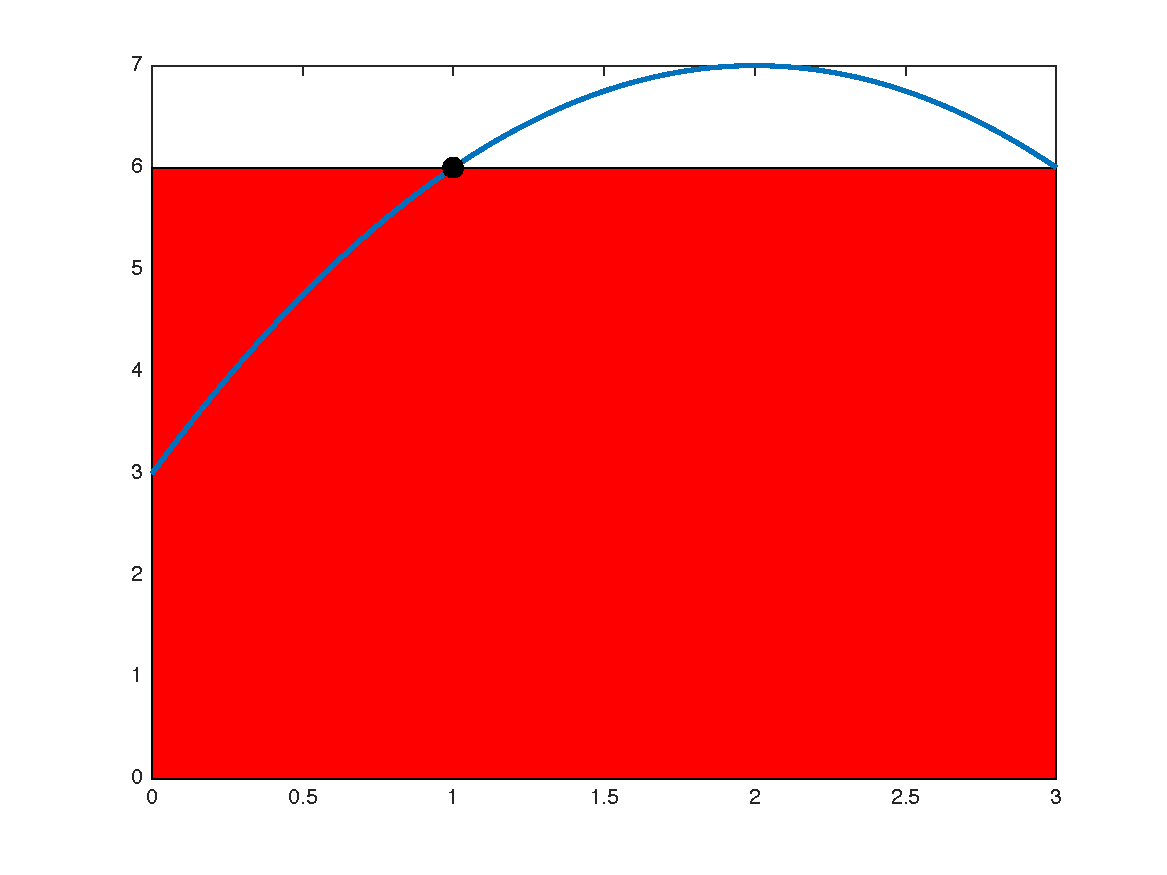
\includegraphics[width =0.5\textwidth]{AC2.pdf}%
%\includegraphics[scale = 1]{eas_boar_1.pdf}%
\label{Sine_waves}%
\end{figure}
\vspace{-.5cm}

\vspace{0.5in}

\newpage

 \noindent
 \section{ Integration: General Examples}





\noindent {\bf An example:}  Find $dy/dx$ from
$$
\int_0^y e^{t^2} d t + \int_0^{\sin x } \cos ^2 t d t=0
$$
Note that
$$
\frac{ d}{ dx} \int_0^{b(x)} f(t) d t =b'(x)f(b(x)).
$$
Differentiate with $x$ on the both side,
$$
\frac{ d y}{ dx}  e^{y^2}+ \cos x \cos^2 (\sin x)=0,
$$
i.e.
$$
dy/dx =- e^{-y^2} \cos x \cos^2 (\sin x).
$$

\vspace{0.2in}



\noindent {\bf An example:} Evaluate  the improper integral
$$
I=\int_0^{a} x^2 \sqrt{ a^2 - x^2 }  \;   dx
$$
i.e.,
\begin{eqnarray}
& I & =\int_{0}^{\pi/2}  (a \sin u)^2 (a \cos x) (a \cos u) du \; \; (x=a \sin u)  \nonumber\\
&   & = \int_{0}^{\pi/2}  a^4 \sin^2 u  \cos^2 u \;  du          \; \;  \nonumber\\
&   & =  \int_{0}^{\pi/2}  \frac{a^4}{8} \sin^2 (2 u)  \;  d( 2 u)          \; \; (t=2u) \nonumber\\
&   & =  \frac{a^4}{8} \int_{0}^{\pi}  \sin^2 t  \;  d t          \; \;  \nonumber\\
&   & =  \frac{a^4}{8} \int_{0}^{\pi} (1- \cos 2 t)/2  \;  d t =
\frac{\pi a^4 }{8 \times 2} = \frac{\pi a^4  }{16}\; \; \nonumber
\end{eqnarray}



\vspace{0.2in}



\noindent {\large \bf  Example:} Evaluate the sum by associating
it with a definite integral
$$
I = \lim_{n \to \infty} \left[ \frac{1^p+2^p+
3^p+...+n^p}{n^{p+1}}  \right]
$$
\begin{eqnarray}
& I & = \lim_{n \to \infty}  \frac{1}{n} \left[   \frac{1^p}{n^p}
+ \frac{2^p}{n^p}+ \frac{3^p}{n^p}+...+ \frac{n^p}{n^p}
\right]     \nonumber\\
&   & = \lim_{n \to \infty} \left[ \sum_{j=1}^{n}
\left( \frac{j}{n}\right)^p \right]  \frac{1}{n}   \nonumber\\
&   & = \int_0^{1} x^p \; dx = \frac{1}{1+p} \nonumber
\end{eqnarray}


\newpage

\vspace{0.2in}



\noindent {\large \bf  Example:} Evaluate the sum by associating
it with a definite integral
$$
I = \lim_{n \to \infty} \left[ \frac{1}{\sqrt{n(n+1)}}
+\frac{1}{\sqrt{n(n+2)}}+\frac{1}{\sqrt{n(n+3)}}+...+\frac{1}{\sqrt{n(n+3n)}}
\right]
$$
\begin{eqnarray}
& I & = \lim_{n \to \infty} \left[ \frac{1}{\sqrt{1+ 1/n}}
+\frac{1}{\sqrt{1+(2/n)}}+\frac{1}{\sqrt{1+(3/n)}}+...+\frac{1}{\sqrt{1+(3n/n)}}
\right]  \frac{1}{n}   \nonumber\\
&   & = \lim_{n \to \infty} \sum_{j=1}^{3n} \left[
\frac{1}{\sqrt{1+ (j/n)}} \right]  \frac{1}{n}   \nonumber\\
&   & = \lim_{n \to \infty} \sum_{j=1}^{3n} f \left( {j}/{n}
\right)  \frac{3}{3n}, \;\; f(x)= \frac{1}{\sqrt{1+ x}}
\nonumber\\
&   & = \int_0^3 \frac{1}{\sqrt{1+ x}} dx, \;\; \left[b=3, a=0,
\Delta
x=\frac{3}{3n}, x_j=\frac{j}{3n}, \right] \; \nonumber\\
&   & =\left[ 2 \sqrt{1+ x} \right]_0^{3} dx=2  \nonumber
\end{eqnarray}


\vspace{0.2in}


\noindent {\large \bf  Example: } Show that
$$
\int_0^{ \sin^2 x} \sin^{-1} \sqrt{t} \; dt +\int_0^{ \cos^2 x}
\cos^{-1} \sqrt{t} \; dt = \frac{\pi}{4}, \;\;  0 < x <
\frac{\pi}{2}
$$
Let
$$
f(x)=\int_0^{ \sin^2 x} \sin^{-1} \sqrt{t} \; dt +\int_0^{ \cos^2
x} \cos^{-1} \sqrt{t} \; dt = \frac{\pi}{4}, \;\;  0 < x <
\frac{\pi}{2}
$$
\begin{eqnarray}
& \frac{d f}{d x} & = \sin^{-1}\sqrt{ \sin^2 x } \; (\sin^2 x)' -
\cos^{-1}\sqrt{ \cos^2 x } \; (\cos^2 x)'   \nonumber\\
&          & = x  \sin 2 x -x  \sin 2 x =0    \nonumber
\end{eqnarray}
$$
f(x)=C, \;\;  0 < x < \frac{\pi}{2}.
$$
\begin{eqnarray}
&  f(\pi/4) & =\int_0^{1/2} \sin^{-1} \sqrt{t} \; dt +\int_0^{1/2}
\cos^{-1} \sqrt{t} \; dt  \nonumber\\
&          & =\left[ t \sin^{-1} \sqrt{t} \; dt + \cos^{-1}
\sqrt{t}\right]_0^{1/2}- \int_0^{1/2} t\left[\frac{1}{ \sqrt{1-t}
} - \frac{1}{ \sqrt{1-t}}  \right] dt  \nonumber\\
&          & =  (1/2) \sin^{-1} \frac{1}{ \sqrt{2}}  + (1/2)
\cos^{-1} \frac{1}{ \sqrt{2}} = (1/2) \left( \frac{\pi}{ 4} +
\frac{\pi}{ 4} \right) = \frac{\pi}{ 4}  \nonumber
\end{eqnarray}

\vspace{0.2in}


\newpage


\noindent {\large \bf  Example:} Evaluate the improper integral
$$
I_n = \int_0^{\infty} x^n  e^{-x} \;  dx
$$
\begin{eqnarray}
& I_n & = -\int_0^{\infty} x^n  d e^{-x}    \nonumber\\
&   & = - \left[ x^n  e^{-x} \right]_0^{\infty} + n \int_0^{\infty} x^{n-1}   e^{-x} \; dx  \nonumber\\
&   & = 0+ n I_{n-1}   \nonumber
\end{eqnarray}
i.e.,
$$
I_n=n I_{n-1}=n (n-1) I_{n-2}=n (n-1)(n-2) I_{n-3}=...=n!
$$

\vspace{0.2in}


\noindent {\large \bf  Example:} Evaluate the indefinite integral
$$
\int \frac{x e^x}{\sqrt{e^x-1} } dx
$$
\begin{eqnarray}
& I & =\int \frac{x e^x}{\sqrt{e^x-1} } \;  dx  \nonumber\\
&   & =\int 2x d \sqrt{e^x-1}   \nonumber\\
&   & = 2 x \sqrt{e^x-1}-2 \int \sqrt{e^x-1} \; dx \;\; \left[
t=\sqrt{e^x-1},\; x=\ln(t^2+1)\;
dx = \frac{2t \; dt}{1+t^2}\right]  \nonumber\\
& &  \int  \sqrt{e^x-1} \; dx =\int \frac{2t^2 \; dt}{1+t^2}= \int
\frac{2(t^2+1)-2 \; dt}{1+t^2}=2t-2\tan^{-1}t+C
\nonumber\\
& I  & = 2 x \sqrt{e^x-1}-4 \left( \sqrt{e^x-1} -
\tan^{-1}\sqrt{e^x-1} \right) +C \nonumber
\end{eqnarray}


\vspace{0.2in}






\bigskip

\noindent {\large \bf  Example: }Evaluate the indefinite integral
$$
\int   \frac{ \sin x}{a \sin x+ b\cos x  } dx, \;\; a \ne 0, b \ne
0; ;
$$
Let
$$
T_s =\int   \frac{ \sin x}{a \sin x+ b\cos x  } dx, \;\; T_c =
\int \frac{ \cos x}{a \sin x+ b\cos x  } dx.
$$
Hence
\begin{eqnarray}
& aT_s+ bT_c & = x +C_1    \nonumber\\
& aT_c - b T_s  & = \int   \frac{ a \cos x - b \sin x}{a \sin x+ b\cos x  } dx      \nonumber\\
&  &            = \int   \frac{ d( a \sin x + b \cos x)}{a \sin x+ b\cos x  } dx      \nonumber\\
&  &            = \ln  | a \sin x + b \cos x | +C_2
\end{eqnarray}
Solve the above two equations, we obtain
\begin{eqnarray}
& T_s  & =   \frac{1}{a^2 +b^2} \left( a x -b \ln  | a \sin x + b \cos x | +C \right)      \nonumber\\
& T_c  & =    \frac{1}{a^2 +b^2} \left( b x +a \ln  | a \sin x + b
\cos x | +C \right)      \nonumber
\end{eqnarray}



\vspace{0.2in}

\newpage

\noindent {\large \bf  Example:} Evaluate the improper integral
$$
I = \int_0^2  \frac{d x}{\sqrt{x (2-x)}}.
$$
\begin{eqnarray*}
& I & = \int_0^1  \frac{d x}{\sqrt{x (2-x)}} + \int_1^2
\frac{d x }{\sqrt{x (2-x)}} \\
&  & = \lim_{\epsilon_1 \to 0} \int_{\epsilon_1}^1
\frac{dx}{\sqrt{x (2-x)}} + \lim_{\epsilon_2 \to 0}
 \int_{1}^{2-\epsilon_2} \frac{dx}{\sqrt{x (2-x)}}\\
 &  & = \lim_{\epsilon_1 \to 0} 2 \int_{\epsilon_1}^1
\frac{d \sqrt{x} }{\sqrt{(2-x)}} + \lim_{\epsilon_2 \to 0}
 2 \int_{1}^{2-\epsilon_2}  \frac{d\sqrt{x}}{\sqrt{(2-x)}}\\
  &  & = \lim_{\epsilon_1 \to 0} 2 \int_{\epsilon_1}^1
\frac{d \sqrt{x/2} }{\sqrt{(1-x/2)}} + \lim_{\epsilon_2 \to 0}
 2 \int_{1}^{2-\epsilon_2}  \frac{d\sqrt{x/2}}{\sqrt{(1-x/2)}}\\
 &  & = \lim_{\epsilon_1 \to 0} 2 \sin^{-1} \left[ \frac{\sqrt{x} }{\sqrt{2} }
 \right]_{\epsilon_1}^1 + \lim_{\epsilon_2 \to 0} 2 \sin^{-1} \left[ \frac{\sqrt{x} }{\sqrt{2} }
 \right]_1^{2-\epsilon_2}\\
  &  & = \lim_{\epsilon_1 \to 0} 2
  \left[ \frac{\pi}{4}- \sin^{-1} \sqrt{\epsilon_1/2} \right]
 + \lim_{\epsilon_2 \to 0} 2
  \left[\sin^{-1} \sqrt{(2-\epsilon_2)/2} -\frac{\pi}{4}
  \right]\\
   &  & =  \frac{\pi}{2}+ 2
  \left( \frac{\pi}{2} -\frac{\pi}{4}
  \right)= \pi
\end{eqnarray*}

\bigskip

\noindent {\large \bf  Example:} Evaluate the improper integral
$$
I = \int_{1/2}^{3/2}  \frac{d x}{\sqrt{|x-x^2|} }.
$$
\begin{eqnarray*}
& I & = \int_{1/2}^{1}  \frac{d x}{\sqrt{x-x^2} }+ \int_{1}^{3/2}  \frac{d x}{\sqrt{x^2-x} }=I_1+I_2\\
& I_1 & = \int_{1/2}^{1}  \frac{d (2x)}{\sqrt{1- (4x^2-4x+1)}}=
\int_{1/2}^{1} \frac{d (2x-1) }{\sqrt{1-(2x- 1)^2}
}=\sin^{-1}[2x-1]_{1/2}^{1}=\sin^{-1} 1=\pi/2 \\
& I_2 & =\int_{1}^{3/2}  \frac{d x}{x^2-x }= \int_{1}^{3/2}
\frac{d (2x-1)}{\sqrt{(4x^2-4x+1)-1}} \\
&=& \cosh^{-1} \left[ 2x-1)\right]_1^{3/2}; \;\;
 [ \cosh^{-1}x=y, e^{2y}-2x e^y+1=0, y=\ln(x+\sqrt{x^2-1})] \\
& & = \left[ \ln((2x-1)+\sqrt{(2x-1)^2-1})\right]_1^{3/2}=\ln
(2+\sqrt{3})-\ln 1=\ln (2+\sqrt{3}).
\end{eqnarray*}
Hence
$$
I_1+I_2= \pi/2+ \ln (2+\sqrt{3}).
$$

\newpage
\section{Integral Test for Infinite Series}

$$
\sum_{n=1}^\infty \frac{1}{n}
\qquad
\sum_{n=1}^\infty \frac{1}{n^2}
$$
$$
\sum_{n=1}^\infty \frac{1}{n^{1+\epsilon}}
\qquad
\sum_{n=2}^\infty \frac{1}{n\ln n}
$$
are all examples of infinite sums
$$
\sum_{n=1}^\infty a_n
$$
where the ratio test \textcolor{red}{fails} because
$$
\lim_{n \rightarrow \infty} \frac{a_{n+1}}{a_n} = 1
$$


\begin{figure}[!ht]
\centering
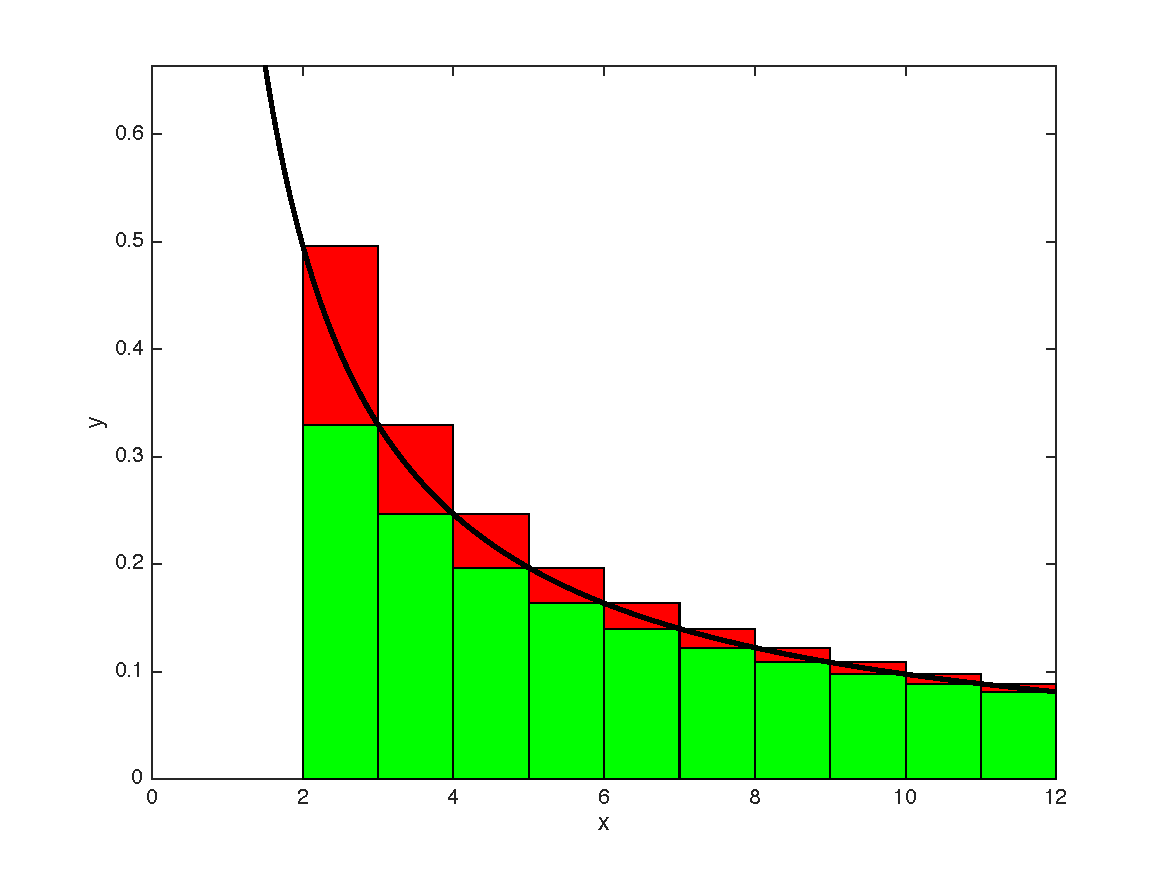
\includegraphics[width = 0.5\textwidth]{AC3.pdf}
\caption{Use "green rectangles'' for convergent sums from finite integrals; Use "red rectangles'' for divergent sums from infinite integrals}
\end{figure}


Let $f(x)$ be non-increasing and non-negative on an unbounded interval $[N, \infty)$. 
$$
{\rm (i)}\,\int_N^\infty f(x) dx < \infty\quad \implies \quad \sum_N^\infty f(n) < \infty
$$
$$
{\rm (ii)}\,\int_N^\infty f(x) dx  = \infty\quad \implies \quad \sum_N^\infty f(n)  = \infty
$$
Proof of (i):
\begin{proof}
Use the \textcolor{green}{right} Riemann (partial) sum.
$$
\sum_N^\infty f(n) = f(N) + \sum_{N+1}^\infty f(n) \leq \int_N^\infty f(x) dx < \infty
$$
\end{proof}
Proof of (ii): 
\begin{proof}
Use the \textcolor{red}{left} Riemann (partial) sum
$$
\sum_N^\infty f(n) \geq \int_N^\infty f(x) dx = \infty
$$
\end{proof}
NB. Here, the width of the ``rectangles'' $\Delta x = 1$.


\subsection{Examples}

$$
\sum_{k=1}^\infty \frac{1}{k^p} \quad \mbox{is finite if, and only if,} \quad p > 1\,.
$$
Proof
$$
\int_1^L x^{-p} dx = 
\left\{ \begin{array}{l} 
\frac{1}{1-p} \left( L^{1-p} - 1\right) \mbox{ if } p \neq 1\\ 
\\
\ln(L) \mbox{ if } p = 1
\end{array} \right.
$$
If $p > 1$, then 
$$
\lim_{L \rightarrow \infty} \int_1^L x^{-p} dx = \frac{1}{p-1} < \infty\,.
$$
If $p \leq 1$, then
$$
\lim_{L \rightarrow \infty} \int_1^L x^{-p} dx = \infty\,.
$$
Result follows by applying the integral test.


\subsection{Estimating infinite sums}

Using the idea that underpins the ``Integral Test'' we can obtain numerical approximations to
``tricky'' infinite sums. 

For example, using some fancy mathematics (see the module \textit{Data Signals and Systems}) we can show that
$$
\sum_{n=1}^\infty \frac{1}{n^4}= \frac{\pi^4}{90}
$$
For the moment, we can estimate this sum: Let
$$
S := \sum_{n=1}^\infty \frac{1}{n^4} \mbox{   and   } S_N = \sum_{n=1}^N \frac{1}{n^4}
$$
Then 
$$
S-S_N = \sum_{n=N+1}^\infty \frac{1}{n^4}
$$


Clearly, we can link
$$
\sum \frac{1}{n^4} \mbox{   and   } \int \frac{1}{x^4} dx\,.
$$
Indeed, using Riemann partial sums we have
$$
\left[ \frac{-1\,\,}{3 x^3} \right]_{N+1}^\infty = \int_{N+1}^\infty \frac{1}{x^4} dx \leq \sum_{n=N+1}^\infty \frac{1}{n^4} \leq  \int_N^\infty \frac{1}{x^4} dx = \left[ \frac{-1\,\,}{3 x^3} \right]_{N}^\infty 
$$
It follows that
$$
 \frac{1}{3(N+1)^3} \leq \sum_{n=N+1}^\infty \frac{1}{n^4} \leq  \frac{1}{3N^3}
 $$
 so that 
 $$
 \frac{1}{3(N+1)^3} \leq S-S_N \leq  \frac{1}{3N^3}
 $$


Using some simple Matlab code we have that:
%
%\begin{figure}%
%\vspace{-.2cm}
%\includegraphics[width = 4cm]{sumnpower4.pdf}%
%%\includegraphics[scale = 1]{eas_boar_1.pdf}%
%\label{Sine_waves}%
%\end{figure}
%\vspace{-.5cm}


%
%\lstset{language=Python}
%\begin{lstlisting}
%>> N=1:6; 1./(3*N.^3)
%>> M=6; S=[ ]; s=0; for i=1:M, s=s+1/(i^4); S=[S  s]; end;
%\end{lstlisting}

\begin{table}[!ht]
\caption{Values of $1/3N^3$ and $S_N$ for various $N$}
\begin{center}
\begin{tabular}{|c|c|c|c|c|c|cl}
$N$ &1 & 2 & 3 & 4 & 5 & 6\\$1/3N^3$ & 0.3333  &  0.0417  &  0.0123  &  0.0052  &  0.0027  &  0.0015\\
$S_N$ & 1.0000  &  1.0625  &  1.0748  &  1.0788  &  1.0804  &  1.0811
\end{tabular}
\end{center}
\label{default}
\end{table}%
So, for example,
{\small 
$$
\hspace{-0.5cm}
\underbrace{1.0804 +  0.0015}_{{\displaystyle \textcolor{red}{1.0819}}} = \overbrace{S_5}^{1.0804}+\overbrace{\frac{1}{3 \times 6^3}}^{0.0015} \leq \sum_{n=1}^\infty \frac{1}{n^4} \leq \overbrace{S_5}^{1.0804}+\overbrace{\frac{1}{3 \times 5^3}}^{0.0027} = \underbrace{1.0804 + 0.0027}_{{\displaystyle \textcolor{red}{1.0831}}}
$$
}
In fact
$$
\sum_{n=1}^\infty \frac{1}{n^4}= \frac{\pi^4}{90} = 1.082323233711138\ldots
$$ 

\section{Estimating $N!$}

$2! = 2$, $3! = 3 \times 2 \times 1 = 6$, $N! = N \times (N-1)!$.

So how big is $N!$. Well
$$
\begin{array}{ll}
\ln N! & = \ln N + \ln (N-1) + \ldots + \ln 2 + \ln 1 \\ 
& \leq \int_1^{N+1} \ln x dx  = \left( x \ln x - x \right)_1^{N+1}
\end{array}
$$
whilst
$$
\begin{array}{ll}
\ln N! & = \ln N + \ln (N-1) + \ldots + \ln 2 + \ln 1 \\
& \geq \int_1^{N} \ln x dx  = \left( x \ln x - x \right)_1^{N}
\end{array}
$$
It follows that
$$
N \ln N -N + 1 \leq \ln N! \leq (N+1) \ln (N+1) - N
$$
or, exponentiating:
$$
e \left( \frac{N}{e} \right)^N \leq n! \leq  e \left( \frac{N+1}{e} \right)^{N+1} 
$$

Also we can estimate the number of permutations of a standard deck of 52 playing cards:
$$
1.2110 \times 10^{67} < \textcolor{red}{52!} < 6.3578 \times 10^{68}
$$

\newpage

\part{Differential Equations}

\section{Basic Definitions}
\subsection{What is a differential equation?}

\begin{itemize}
\item
\textbf{A differential equation}: An equation containing an
unknown function and one or more of its derivatives.
\item
\noindent The {\bf order of a differential equation}: the highest
order derivative that occurs in the equation.
\item
\noindent {\bf A linear ordinary differential equation of order
$n$} may be written as:
$$
p_0(x) \frac{ d^n y}{d x^n} +p_1(x) \frac{ d^{n-1} y}{d x^{n-1}}
+p_2(x) \frac{ d^{n-2} y}{d x^{n-2}}+\ldots + p_n(x) y(x)=r(x);
$$
$y$ is the dependent variable, $ x$ is the independent variable.
\item
\noindent {\bf A nonlinear differential equation}: An equation
that cannot be put in the above form.
\item
\noindent {\bf Homogeneous  differential equation}: $r(x)=0$.
\item
\noindent {\bf Inhomogeneous  differential equation}: $r(x) \ne 0.$
\end{itemize}


\subsection{Motivating Examples}

\begin{itemize}
\item
\textbf{Falling under constant gravity}
$$
m \frac{d^2h}{dt^2} (t) = -mg \quad (\mbox{Newton's falling apple})
$$
\item
\textbf{Newton's Law of Cooling}
$$
\frac{dT_{in}}{dt} = c (T_{out} - T_{in}) \quad (\mbox{recall climate change energy balance})
$$
\item
\textbf{Cash in the bank}
$$
\frac{dc}{dt} = r c\quad \mbox{interest rate } r
$$
\item
\textbf{Mass on the end of a spring}
$$
m \frac{d^2 x}{dt^2} = -k x \quad (\mbox{Newton + Hooke})
$$
\end{itemize}


\subsection{What is the solution of a differential equation}

\begin{itemize}
\item
\noindent {\bf General solution}: General solution of an $n$th
order ODE contains $n$ arbitrary constants. If $n$ boundary conditions
are specified, these $n$ arbitrary constants can be determined.
\item
\noindent {\bf Particular  solution}: A particular  solution is
obtained from a general solution by assigning particular values of
the arbitrary constants.
\end{itemize}


\subsection{Linear or Nonlinear DEs}

\textbf{Example D1}: The differential equation
$$
 \frac{ d^2 y}{d x^2} +4 x \frac{ d y}{d x}+ 2y= \cos x
$$
is (i) linear, (ii) second order and (iii)  inhomogeneous.
Linearity is determined solely by the way that the dependent variable
$y$ and its derivative occur in the equation.

\textbf{Example D2}: The differential equation
$$
 \frac{ d^2 y}{d x^2} + \sin y = 0
$$
is second order and nonlinear because of the term $\sin y$.


\section{First Order Differential Equations}
\subsection{Separable equations}

\textcolor{red}{Separation of variables} is a key approach to solving differential equations. A separable
differential equations takes the form:
$$
\frac{dy}{dx} = \frac{f(x)}{g(y)}, \;\; \mbox{or} \;\; g(y)\; dy =  f(x)
\, dx.
$$
The general solution of such separable ODEs are obtained by integration:
$$
\int {g(y)}\, dy  = \int f(x) \, dx.
$$
When/if these integrals have been done, the constant of integration
gives the one arbitrary constant required for the general
solution. If a condition is specified, use it to determine the
value of the constant to get the Particular Solution.

\hrulefill

\textbf{Example D3.}: Solve the differential equation
$$
\frac{dy}{dx} = \frac{1-y^2}{y(1-x)}
$$
Separating the terms $x$, $dx$ and $y$, $dy$ gives
$$
\frac{y}{1-y^2} dy = \frac{1}{1-x} dx
$$
so that
$$
\int \frac{ y \; dy}{(1-y^2)}= \int \frac{dx}{(1-x)} \mbox{ or } \int - \frac{1}{2}\frac{d(1-y^2)}{1-y^2}= -\int \frac{d(1-x)}{(1-x)}
$$
Integrating the above equation, we obtain an equation defining $y$
as an implicit function of $x$:
$$
\ln |1-y^2|= 2 \ln |1-x| -C,
$$
i.e.
$$
\ln \frac{|1-x|^2}{|1-y^2|}= C, \;\;
\frac{|1-x|^2}{|1-y^2|}=e^C=k^2, \;\; k^2 \ne 0
$$


Clearing the fractions and eliminating the absolute values gives:
$$
(1-x)^2 = \lambda  (1-y^2),  \;\; \lambda= \pm k^2 \ne 0; \;\;
\frac{(x-1)^2}{\lambda}+y^2=1
$$
where $\lambda$ takes on any real value, except for $0$. If $
\lambda >0$, the solution curves are all ellipses; If $ \lambda
<0$, the solution curves are all hyperbolas.

For example, the particular solution passing through the point $(x=0,
y=0)$, we then have $ \lambda=1$ giving
$$
(x-1)^2+y^2=1.
$$


\subsection{First order homogeneous differential equations}


The first order differential equation
$$
\frac{dy}{dx} = F(x,y)
$$
is homogeneous in $x$ and $y$ when
$$
F(\alpha x, \alpha y)
$$ 
is independent of $\alpha$. In this case,
$$
F(x,y) = f\left( \frac{y}{x}\right) 
$$
To see this put $\alpha = \frac{1}{x}$. Then
$$
F(x,y) = F(\alpha x, \alpha y) = F\left( 1,\frac{y}{x}\right)  = f\left( \frac{y}{x}\right)   
$$
So DEs with homogeneous $F(x,y)$ have a ``standard form''
$$
\frac{d y}{dx} = f\left( \frac{y}{x}\right) 
$$


Using the substitution $u = \frac{y}{x}$ gives 
$$
y = u x
$$ 
and 
$$
\frac{d y}{dx} = x \frac{du}{dx} + u = f(u)
$$
Hence the differential equation 
$$
\frac{d y}{dx} = f(\frac{y}{x})
$$
in $x$ and $y$ simplifies to a \textcolor{red}{separated} equation
$$
x \frac{du}{dx} = f(u) - u \mbox{ or } \frac{du}{f(u) - u} = \frac{dx}{x}
$$
in $x$ and $u$.

\hrulefill

\textbf{Example D4.} Solve the differential equation
$$
\frac{dy}{dx} = \frac{x^2 +3 y^2}{2 xy}\,.
$$
We write the DE in standard form by dividing top/bottom by $x^2$:
$$
\frac{dy}{dx}= \frac{x^2 +3 y^2}{ 2 xy }= \frac{1 +3 {y^2/x}^2}{ 2 (y/x)} = \frac{1 +3 {u}^2}{ 2u} .
$$
With
$$
y=x\, u(x), \; \; \frac{d y}{d x}= \; x\frac{d u}{d x}+u \;\; %\mbox{ or }dy=udx +x du
$$
$$
x\frac{d u}{d x}+ u = \frac{dy}{dx} = \frac{1 + 3 u^2}{ 2u} \implies 
\textcolor{red}{x \frac{d u}{dx}} = \frac{1 + 3 u^2}{ 2u} - u= \textcolor{red}{\frac{1 +  u^2}{ 2u}}
$$


Separating variables, we obtain
$$
\frac{dx}{x}= \frac{2 u\,  du}{1 +  u^2}
$$
then, by integrating, we find
$$
\ln |x| - \ln |1 +  u^2| = C.
$$
This can be written as
$$
\ln \left| \frac{x}{1+u^2} \right| =\ln e^C, \;\;
$$
Clearing of fractions and eliminating the absolute value
$$
\left| \frac{x}{1+(y/x)^2} \right| = k^2, \;\; k^2=e^C, \;\;
\frac{x}{1+(y/x)^2}  = \pm k^2.
$$
Note that $k=0, (x=0)$ is also a solution of the given equation.


\subsection{Linear first order differential equations} 

Linear first order inhomogeneous DEs can be written in the form
$$
\frac{dy}{dx} + p(x) y = r(x).
$$
To solve these equations we use the \textcolor{red}{integrating factor} method. We multiply the DE by the ``integrating'' factor
$$
u (x) = \exp \int p \, dx.
$$
Then 
$$
\begin{array}{ll}
\textcolor{red}{\frac{d}{dx}( u(x) y(x) )} & = \frac{du}{dx} y(x) + u(x) \frac{dy}{dx} \\
\\
& = p(x) u(x) y(x) + u(x) \left(r(x) - p(x) y(x) \right) = \textcolor{red}{u(x) r(x)}\,.
\end{array}
$$
It follows that
$$
u(x)y(x) = \int u(x) r(x) \, dx +C\,.
$$


This means that
$$
y(x) = \int \left[ \left( e^{\int p(x) \, dx} \right) r(x) \, dx
+C \; \right] e^{-\int p(x) \, dx}.
$$
is the \textcolor{red}{general solution} of the linear first order inhomogeneous DE
$$
\frac{dy}{dx} + p(x) y = r(x).
$$

\hrulefill

\textbf{Example D5.} Find the solution of the differential equation
$$
\frac{dy}{dx} - \frac{ 2x}{1 +x^2 }y=1, \quad y(0) = 1
$$
The integrating factor $u(x)$ is
{\small 
$$
\exp \left( - \int \frac{ 2x}{1 +x^2 } \, dx \right)=\exp \left( - \ln (1 +x^2)\right)=\frac{1}{\exp(\ln(1+x^2))} = \frac{1}{1 +x^2 }.
$$
}
Multiplying the equation by this factor
$$
\frac{ 1}{1 +x^2 } \frac{dy}{dx} - \frac{ 2x}{(1 +x^2)^2 }y=\frac{d}{d x } \left( \frac{ y}{1 +x^2 } \right) =\frac{ 1}{1 +x^2 }.
$$
Integrating
$$
\left( \frac{ y}{1 +x^2 } \right) = \int \frac{ 1}{1 +x^2 } \; dx= \tan^{-1} x+C.
$$
When $x=0, y=1$ so that
$$
C = 1, \;\; \mbox{and } y(x)= (1 +x^2 )(\tan^{-1} x+1).
$$


\section{Linear Second Order Differential Equations}
\subsection{Formulation}
 
The general second order linear differential equation has the form
$$
\frac{d^2 y}{dx^2} + p(x) \frac{dy}{dx} + q(x) y = r(x).
$$
where $p(x)$ and $q(x)$ are coefficient functions.

When $r(x)=0$, the equation is homogeneous
$$
\frac{d^2 y}{dx^2} + p(x) \frac{dy}{dx} + q(x) y = 0.
$$
If $y_1(x)$ and $y_2(x)$ are \textcolor{red}{linearly independent solutions} of the equation, 
then the general solution is given by
$$
y(x)=C_1 y_1(x) + C_2 y_2(x)
$$
where $C_1$ and $C_2$ are arbitrary constants. 



\textbf{Independence of functions}: A set of functions $\left\{ y_1 (x), \ldots, y_k (x) \right\}$ are linearly independent\footnote{See extra notes on linear independence of functions for more info}
if
$$
c_1 y_1(x) + \ldots + c_k y_k (x) = 0, \mbox{ for all } x
$$
means 
$$
c_1 = \ldots = c_k = 0\,.
$$
For example $\sin x$ and $\cos x$ are linearly independent. Indeed, if
$$
c_1 \sin x + c_2 \cos x \equiv 0, \quad x = 0 \implies c_2 = 0, \quad x = \frac{\pi}{2} \implies c_1 = 0\,.
$$ 
The monomials $y_1 (x) = 1, y_2 (x) = x, \ldots , y_k = x^{k-1}$ are linearly independent also.

There is no general, closed form solution for linear differential equations with 
non-constant coefficients and approaches to sol. However, there is ``analytical'' mileage in rewriting the second
order DE in first order form by setting
$$
z(x) = \left( \begin{array}{l} y(x) \\ y'(x) \end{array} \right) \qquad \mbox{so that}
$$
{\small
$$
z'(x) = \left( \begin{array}{l} y'(x) \\ y''(x) \end{array} \right) = \left( \begin{array}{cc} 0 & 1 \\ -q(x) & -p(x) \end{array} \right) \left( \begin{array}{l} y(x) \\ y'(x) \end{array} \right) + \left( \begin{array}{l} 0 \\ 1 \end{array} \right) r(x)
$$
}

\subsection{Using one solution to find another}

Let $y_1 (x)$ be a solution of the homogeneous DE:
$$
\frac{d^2 y}{dx^2} + p(x) \frac{dy}{dx} + q(x) y = 0.
$$
Using $y_1(x)$ we seek a second solution in the form
$$
y(x)= v(x) y_1(x).
$$
If we can find $v(x)$, then we have $y(x)$ and the problem is solved.  First we have that
$$
\frac{d y}{dx}=v\frac{d y_1}{dx}+ \frac{d v}{dx}  y_1;\;\;
\frac{d^2 y}{dx^2}=v\frac{d^2 y_1}{dx^2}+ 2\frac{d v}{dx}\frac{d
y_1}{dx} + \frac{d^2 v}{dx^2}  y_1
$$
So that substituting $y=v \, y_1$ into the equation gives
$$
v \left(\textcolor{red}{\frac{d^2 y_1}{dx^2} + p(x) \frac{dy_1}{dx} + q(x) y_1}\right) + y_1 \frac{d^2 v}{dx}+ \left(2 \frac{d y_1}{dx}+ p y_1
\right) \frac{d v}{dx}=0
$$

But $y_1 (x)$ is a solution, i.e.
$$
\frac{d^2 y_1}{dx^2} + p(x) \frac{dy_1}{dx} + q(x) y_1 = 0\,.
$$
It follows that
$$
 y_1 \frac{d^2 v}{dx}+ \left(2 \frac{d y_1}{dx}+ p y_1
\right) \frac{d v}{dx}=0
$$
or
$$
\frac{v''}{v'}= -2 \frac{ y_1'}{y_1}-p(x), \;\; \frac{ d v'}{v'}=
-2 \frac{ d y_1}{y_1}- p(x) dx.
$$
An integration gives
$$
\ln v'= -2 \ln y_1 - \int p(x) dx, \;\;   \implies \,\, v' y_1^2= e^{- \int
p(x) dx}
$$
and hence
$$
 v= \int \left( y_1^{-2}  e^{- \int p(x) dx} \right) dx
$$

\hrulefill

\textbf{Example D6.}: Find the general solution of the
differential equation
$$
x^2 y''(x) + xy' (x) -y (x)=0 \quad \mbox{i.e.} \quad y''(x) + \frac{1}{x} y' (x) - \frac{1}{x^2} y (x)=0
$$
By inspection, \textcolor{red}{$y_1=x$} is a solution of the equation. In this case
$$
p(x) = \frac{1}{x} \mbox{  and  } q(x) = -\frac{1}{x^2}
$$
So a second linearly independent solution is then given by \textcolor{red}{$y_2=v(x) y_1$} with
{\small
$$
\begin{array}{lll}
 v & = & \int \left( y_1^{-2}  e^{- \int p(x) dx} \right) dx =  \int \left( x^{-2}  e^{- \int (1/x) dx} \right) dx \\
 \implies v & = & \int \left( x^{-2}  e^{-\ln x}  \right) dx =\int \left( x^{-2} x^{-1}  \right) dx
 =- x^{-2}/2
 \end{array}
$$
}
This yields
$$
\textcolor{red}{y_2 = x \, v=- x^{-\frac{1}{2}}}
\quad \mbox{ and a general solution} \quad 
y(x)=C_1 x + C_2  x^{-1}.
$$

% END OF ODES PART 1

\bigskip

\noindent {\bf  Homogeneous equation with constant coefficients}
Standard form is
$$
\frac{d^2 y}{dx^2} + p \frac{dy}{dx} + q  y = 0,
$$
where $p$ and $q$ are constants. Consider $ y=e^{mx}$ as a
possible solution. Substitution yields
$$
\left(m^2+ pm + q \right)e^{mx}=0, \;\;  \to \;\; \left(m^2+ pm +
q \right)=0,
$$
which is called the auxiliary equation (or characteristic
equation) (since $e^{mx}$ is never zero).\\
The two roots $m_1, m_2$ are are given by the quadratic formula
$$
m_{1,2} = \frac{ -p \pm \sqrt{p^2- 4q} }{2}.
$$

\bigskip
\hrulefill

\noindent {\bf Distinct real roots when $(p^2- 4q)>0$.} In this
case, we get the two linearly independent solutions
$$
y_1= e^{m_1 x}, \;\; y_2= e^{m_2 x}
$$
and the general solution is
$$
y(x)= C_1 e^{m_1 x} +C_2  e^{m_2 x}.
$$

\hrulefill

\noindent {\bf Distinct complex roots when $(p^2- 4q)<0$.} In this
case,
$$
m_1=a+ib=\frac{ -p + i\sqrt{|p^2- 4q}| }{2}; \;\; m_2=a-ib=\frac{
-p - i\sqrt{|p^2- 4q}| }{2}
$$
we get the two linearly independent solutions
$$
y_1= e^{(a+ib) x}=e^{a x}( \cos bx +i \sin b x) , \;\; y_2=
e^{(a-ib) x}=e^{a x}( \cos bx -i \sin b x) , \;\;
$$
and the general solution is
$$
y(x)=e^{a x}\left[  C_1( \cos bx +i \sin b x)+ C_2( \cos bx -i
\sin b x) \right]=e^{a x}\left(  c_1 \cos bx +c_2 \sin b x \right)
$$
where $c_1=C_1+C_2; \;\; c_2=i(C_1-C_2)$.

\bigskip
\hrulefill

\noindent {\bf Equal real roots when $(p^2- 4q)=0$.} In this case
($m_1=m_2=m=-p/2$), we get the two linearly independent solutions
$$
y_1= e^{m x}, \;\; y_2= x e^{m x}
$$
and the general solution is
$$
y(x)= C_1 e^{m x} +C_2 x e^{m x}
$$
From the first known solution, we can easily find a second
linearly independent solution by
$$
y_2=vy_1=v(x) e^{mx},
$$
where
$$
 v= \int \left( (y_1)^{-2}  e^{- \int p dx} \right) dx=
 \int \left( (e^{-px/2})^{-2}  e^{- \int p dx} \right) dx=
  \int \left( (e^{p x}  e^{-p dx} \right) dx=x.
$$

\bigskip

\newpage

\noindent {\bf Initial-value  problems.} It consists of finding a
solution of $y$ that satisfies initial conditions of the form
$$
y(a)=A, \;\; y'(a)=B,
$$
where $A$ and $B$ are given constants. \\
\noindent {\bf Boundary-value problems.} It consists of finding a
solution of $y$ that satisfies boundary conditions of the form
$$
y(a)=A, \;\; y(b)=B,
$$
where $A$ and $B$ are given constants.

\hrulefill
\bigskip

\noindent {\bf Example}: Solve the initial-value problem
$$
y''+ y=0 \;\; y(0)=2 \;\; y'(0)=3
$$
The auxiliary equation is ,
$$
m^2+1=0
$$
whose roots are $m_1=i, m_2=-i$. The general solution is
$$
y(x)=c_1 \cos x + c_2 \sin x
$$
$$
y'(x)= -c_1 \sin x + c_2 \cos x
$$
This yields
$$
y(0)=c_1=2, \;\;  y'(0)=c_2=3.
$$
Therefore,  the  solution of the initial value problem is
$$
y(x)=2 \cos x +3 \sin x.
$$

\hrulefill
\bigskip

\noindent {\bf  Inhomogeneous equation with constant coefficients}
Standard form is
$$
\frac{d^2 y}{dx^2} + p \frac{dy}{dx} + q  y = r(x),
$$
where $ r(x) \ne 0$ and $p$ and $q$ are constants.

\bigskip

{\bf The First step} is to solve the equivalent homogeneous problem,
the complementary equation,
$$
\frac{d^2 y}{dx^2} + p \frac{dy}{dx} + q  y = 0,
$$
the obtained by setting $r(x)=0$. Since this equation is linear
and homogeneous, If we find two independent solutions, $y_1(x)$
and $y_2(x)$, the  complementary function is
$$
y_c = C_1 y_1+ C_2 y_2.
$$

\bigskip

\noindent{\bf The Second step} is to find a Particular Integral,
$y_p$. This is basically a matter of trial and error, but the
following guidelines are helpful.

\bigskip

(i) If $r(x)$ is a polynomial of degree $m$, try
$$
y = a_n x^m + a_{n-1} x^{m-1} + \cdots +a_0
$$
and substitute in to the ODE. Equate the powers of $x$ in the
result with $r(x)$ to determine the coefficients. [This is
sometimes called the method of undetermined coefficients].

\bigskip

(ii) If $r(x)$ contains $h e^{\lambda x}$, try for the P.I.
$$
y= a e^{\lambda x}.
$$
Again substitute into the ODE and equate both sides to determine
$a$.

\bigskip

(iii) If $r(x) = C \cos \lambda x + D \sin \lambda x$, try $y = a
\cos \lambda x + b \sin \lambda x$, substitute in and equate
coefficients of $\cos \lambda x$ and $ \sin \lambda x$ to
determine $a$ and $b$.

\bigskip

(iv) If $r(x)$ is any combination of the above, find P.I.'s for
each piece separately, and add to find the full P.I.

\bigskip

(v) If $r(x) = h e^{\lambda x}$ and $e^{\lambda x}$ happens to be
a part of the C.F., try $a x e^{\lambda x}$ instead of $a
e^{\lambda x}$. \\
If $r(x) = he^{\lambda x}$ is a double root of the homogeneous
problem, try $a x^2 e^{\lambda x}$.\\
Similarly,  if $r(x)= \exp(px) [C \cos q x + D \sin q x]$ happens
to be part of the C.F., try $y = x e^{px} (a \cos q x + b \sin q
x)$ for the P.I.

\bigskip

\noindent{\bf The third step}. The general solution of the
nonhomogeneous equation is written as
$$
y(x)=y_p +y_c
$$
Since the complementary function has two arbitrary constants if
the equation is of second order, this general solution has the
correct number of arbitrary constants.

\hrulefill
\bigskip

\noindent {\bf Example}: Solve
$$
y''+ 4 y= e^{3x}.
$$
The auxiliary equation is
$$
m^2+4=0,
$$
whose roots are $m_1=2i, m_2=-2i$. The solution of the
complementary equation is
$$
y_c=c_1 \cos 2 x + c_2 \sin 2 x.
$$
For a particular integral (solution), we try $ y_p= a e^{ 3x}$
(the method of undetermined coefficients)
$$
9 a e^{3x} + 4 a e^{3x} = e^{3 x}, \;\; \to \;\; a =1/13,
$$
leading to the general solution
$$
y=y_p+ y_c= \frac{1}{13} e^{3 x} + c_1 \cos 2 x + c_2 \sin 2 x.
$$


\bigskip
\hrulefill

\noindent {\bf Example}: Solve
$$
y''+  y= \sin x.
$$
The auxiliary equation is
$$
m^2+1=0,
$$
whose roots are $m_1=i, m_2=-i$. The solution of the complementary
equation is
$$
y_c=c_1 \cos  x + c_2 \sin  x.
$$
For a particular integral (solution), we try
$$
y_p=x( a \cos x + b \sin x).
$$
Then
$$\
y_p'= a \cos x + b \sin x + x( -a \sin x + b \cos x)
$$
$$
y_p''= -2a \sin x + 2b \cos x  -a x \cos x - b x \sin x
$$
Substitution in the equation gives
$$
\left( -2a \sin x + 2b \cos x  -a x \cos x - b x \sin x \right) +
\left( a x \cos x + b x \sin x \right)= \sin x,
$$
$$
-2a \sin x + 2b \cos x  = \sin x; \;\; \to \;\; a= -1/2; b=0; \;\;
y_p= -\frac{x}{2} \cos x.
$$
The general solution is
$$
y=y_p+ y_c=  c_1 \cos  x + c_2 \sin  x  -\frac{x}{2} \cos x.
$$


\bigskip
\hrulefill

\noindent {\bf  Higher-order homogeneous equation with constant
coefficients} Standard form is
$$
\frac{d^n y}{dx^n} + a_1 \frac{d^{n-1} y}{dx^{n-1}}+...+ a_{n-1}
\frac{d y}{dx}+  a_n y= r(x),
$$
where $ a_j, j=1,...n$ are  constants.

When $r(x)=0$ (homogeneous equation), consider $ y=e^{mx}$ as a
possible solution. Substitution in the equation leads to the
characteristic equation
$$
m^n+ a_1 m^{n-1} +...+ a_{n-1} m+ a_n =0;
$$
the degree of this algebraic equation will be the same as the
order of the differential equation.  The procedure is similar to
that of the second-order differential equation.

\bigskip
\hrulefill

\noindent {\bf Example} Find the general solution of
$$
y'''+ 3y''+ 3 y' +y=0;
$$
the characteristic equation is
$$
m^3 + 3 m^2 + 3m +1=(m+1)^3=0.
$$
Hence, $m=-1$ is a triple root and three linearly independent
solutions are
$$
y_1= e^{-x}, \;\; y_2= x e^{-x}, \;\; \;\; y_3= x^2 e^{-x}
$$
and the general solution is
$$
y(x)= C_1 e^{-x} +C_2 x e^{-x} +C_3 x^2 e^{-x}.
$$

\hrulefill

\noindent {\bf Example} Find the general solution of
$$
y^{(4)}+32y''+256y=0.
$$
the characteristic equation is
$$
m^4+ 32 m^2 +256=0, \;\;  \to \;\; (m^2+16)^2=0
$$
The double complex roots are $ m_1= i 4,  m_2= i 4, m_3= -i 4,
m_4= -i 4.$ The general solutions of the equation
$$
y=C_1 x \cos 4 x + C_2 x \sin 4 x + C_3 \cos 4 x + C_4 \sin 4 x.
$$


\bigskip

\noindent {\large \bf General Examples and Exercises}

\bigskip


\noindent {\bf Example} Assume that $x^3 e^{-x}$ is a solution of
a fourth-order homogeneous differential equation with constant
coefficients.\\
(i) Find the general solution and  (ii) determine the
corresponding differential equation.

\medskip

If $x^3 e^{-x}$ is a solution, then $x^2e^{-x},xe^{-x} e^{-x} $
are also solutions of the equation, i.e.,
$$
y= C_1 x^3 e^{-x} + C_2 x^2 e^{-x} +C_3 x  e^{-x} +C_4  e^{-x}
$$
The four equal real roots are $-1$, or the characteristic equation
is
$$
(m+1)^4=0
$$
which can be expanded in the form
$$
m^4+ 4 m^3+6m^2+4 m+1=0.
$$
Hence, the corresponding differential equation is
$$
y^{(4)}+4 y'''+ 6y''+4y+y=0.
$$

\bigskip
\hrulefill

\noindent {\bf Exercise} Solve $ y^3 y''+1=0$. \\

\vspace{400px}

\bigskip

\noindent {\bf Example} Solve the second ode
$$
(t-1)\frac{d^2 x}{ d t^2}+ (t+1)\frac{d x}{ d t}+x= 2 t.
$$
Let
$$
y=(t-1)x(t), \; \to \; \frac{d y}{ d t}=x+(t-1)\frac{d x}{ d t}
=x+(t+1)\frac{d x}{ d t} -2 \frac{d x}{ d t},
$$
$$
\frac{d y^2}{ d t^2}=2\frac{d x}{ d t}+(t-1)\frac{d^2 x}{ d t^2},
$$
i.e.,
$$
(t+1)\frac{d x}{ d t} = \frac{d y}{ d t}-x +2 \frac{d x}{ d t},
$$
$$
(t-1)\frac{d^2 x}{ d t^2}=\frac{d y^2}{ d t^2}-2\frac{d x}{ d t},
$$
Substitution in the equation yields
$$
\frac{d y^2}{ d t^2}+\frac{d y}{ d t}= 2 t.
$$
It has the complementary solution
$$
(m^2+m)=0, \;\; m_1=0, \; m_2=-1; \; \; y_c=C_1+C_2 e^{-t}
$$
For a particular solution, try
$$
y_p=At^2+Bt
$$
which leads to
$$
2A+ (2At+B)= 2 t, \; \to \; C=0,\; 2A+B=0,\; 2A=2,
$$
$$
A=1 ,\;\; \; B=-1/2.
$$
The general solution is
$$
y=y_c+y_p=C_1+C_2 e^{-t} + t^2- t/2, \;\; \to \;\; x=\frac{1}{
t-1} \left( C_1+C_2 e^{-t} + t^2- t/2 \right).
$$


\bigskip

\noindent {\bf Example} Solve the third-order ode which has a
known solution $x_1=1/t$
$$
t\frac{d^3 x}{ d t^3}+ 3 \frac{d^2 x}{ d t^2} -t\frac{d x}{ d
t}+x= 0.
$$
Let $ x=y/t$, then
$$
\frac{d x}{ d t} =\frac{1}{ t} \frac{d y}{ d t}- \frac{y}{ t^2}
$$
$$
\frac{d^2 x}{ d t^2} =\frac{1}{ t} \frac{d^2 y}{ d t^2}- \frac{2}{
t^2} \frac{d y}{ d t} + \frac{2 }{ t^3} y
$$
$$
\frac{d^3 x}{ d t^3} =\frac{1}{ t} \frac{d^3 y}{ d t^3}- \frac{3}{
t^2} \frac{d^2 y}{ d t^2} +   \frac{6}{ t^3} \frac{d y}{ d t}-
\frac{6 }{ t^4} y
$$
Substitution then in the equation
$$
\left(  \frac{d^3 y}{ d t^3}- \frac{3}{ t} \frac{d^2 y}{ d t^2} +
\frac{6}{ t^2} \frac{d y}{ d t}- \frac{6 }{ t^3} y \right) +
\left( \frac{3}{ t} \frac{d^2 y}{ d t^2}- \frac{6}{ t^2} \frac{d
y}{ d t} + \frac{6 }{ t^3} y \right) - \left(\frac{d y}{ d t}-
\frac{y}{ t}\right)+ y/t=0
$$
$$
\frac{d^3 y}{ d t^3} -  \frac{d y}{ d t} =0.
$$
Let $ dy/dt=z$, then
$$
\frac{d^2 z}{ d t^2} - z=0
$$
which has the general solution
$$
z= C_1 e^t+C_2 e^{-t}, \; \to \; y= C_1 e^t-C_2 e^{-t} +C_3
$$
$$
x= \frac{1}{t} \left( C_1 e^t-C_2 e^{-t} +C_3\right).
$$



\bigskip

\noindent {\bf Example} Solve the second-order ode
$$
\frac{d^2 y}{ d x^2}+ (x+ e^{2y}) \left( \frac{d y}{ d
x}\right)^3= 0.
$$
Note that
$$
\frac{d y}{ d x} =\left( \frac{ dx }{ dy } \right)^{-1}
$$
$$
\frac{d^2 y}{ d x^2} = \frac{d y' }{d y } \frac{d y }{d x }=
\frac{ d }{ dy } \left( \frac{ 1 }{dx/ dy } \right) \frac{1}{ d
x/dy}= -\left( \frac{ d^2 x/ dy^2 }{(dx/ dy)^2 } \right) \frac{1}{
d x/dy}= - \frac{ d^2 x/ dy^2 }{(dx/ dy)^3 }
$$
Substitution in the equation
$$
- \frac{ d^2 x/ dy^2 }{(dx/ dy)^3 } + (x+ e^{2y}) \left( \frac{ dx
}{ dy } \right)^{-3}=0, \; \to \; -\frac{ d^2 x}{ dy^2 } + (x+
e^{2y})=0
$$
which is a linear equation for $x(y)$
$$
\frac{ d^2 x}{ dy^2 } - x=  e^{2y}
$$
It has the complementary solution
$$
(m^2-1)=0, \;\; m_1=1, \; m_2=-1; \; \; x_c=C_1 e^{y}+C_2 e^{-y}
$$
For a particular solution, try
$$
x_p=A e^{2y}
$$
which leads to
$$
4A -A = 1, \; \to \;   A=1/3.
$$
The general solution is
$$
x=x_c+x_p=C_1 e^{y}+C_2 e^{-y}+ e^{3y}/3.
$$

\noindent {\bf Exercise} Solve the second-order ode
$$
(x+1)\frac{d^2 y}{ d x^2}+  \frac{d y}{ d x}= \ln(x+1).
$$

\newpage

\section{Linear Differential Equations with Constant Coefficients}
\subsection{Second Order Recap}
The standard form is
$$
\frac{d^2 y}{dx^2} + p \frac{dy}{dx} + q  y = 0,
$$
where $p$ and $q$ are constants. 

We seek two linearly independent solutions. 

Inspired guesswork suggests trying a solution $y(x) =e^{mx}$. Substitution yields
$$
\left(m^2+ pm + q \right)e^{mx}=0
$$
Since $\exp(x) \not\equiv 0$, $e^{mx}$ is a solution if, and only if, $m$ satisfies:
$$
m^2+ pm + q=0\,. \qquad \qquad \mbox{Auxiliary Equation}
$$
How we continue depends on the nature of the roots of the \textcolor{red}{auxiliary equation}
$$
m_1, m_2= \frac{1}{2}\left( -p \pm \sqrt{p^2- 4q} \right).
$$

\begin{itemize}
\item
\textbf{Case 1}: Auxiliary equation has \textcolor{red}{distinct real roots}.

If \textcolor{red}{$p^2- 4q>0$} then $m_1$ and $m_2$ are real and distinct. 

In this case, we obtain the two \textcolor{red}{linearly independent} solutions
$$
y_1= e^{m_1 x}, \;\; y_2= e^{m_2 x}
$$
and a general solution
$$
y(x)= C_1 e^{m_1 x} +C_2  e^{m_2 x}.
$$
\end{itemize}


\begin{itemize}
\item
\textbf{Case 2}: Auxiliary equation has \textcolor{red}{distinct complex roots}.

If \textcolor{red}{$p^2- 4q<0$} then $m_1 = a+ib$ and $m_2 = a-ib$ are distinct, non real complex conjugates.

In this case we obtain the two linearly independent solutions
$$
\begin{array}{lll}
y_1 & = & e^{(a+ib) x}=e^{a x}( \cos bx +i \sin b x) \\
y_2 & = & e^{(a-ib) x}=e^{a x}( \cos bx -i \sin b x)
\end{array}
$$
and the general solution is
$$
\begin{array}{lll}
y(x) & = & e^{a x}\left[  C_1( \cos bx +i \sin b x)+ C_2( \cos bx -i
\sin b x) \right] \\ & = & c_1 e^{a x} \cos bx +c_2 e^{ax} \sin b x
\end{array}
$$
\vspace{-5mm}

where $c_1=C_1+C_2; \;\; c_2=i(C_1-C_2)$.

Note that whilst the auxiliary equation has non-real roots, we do end up with two independent
\textcolor{red}{real valued} solutions.
\end{itemize}


\begin{itemize}
\item
\textbf{Case 3}: Auxiliary equation has \textcolor{red}{equal real roots}.

If \textcolor{red}{$p^2- 4q=0$}, then $m_1=m_2=m=-p/2$

In this case we get the two linearly independent solutions
$$
y_1= e^{m x}, \;\; y_2= x e^{m x}
$$
and the general solution is
$$
y(x)= C_1 e^{m x} +C_2 x e^{m x}
$$
To see how we obtain the solution \textcolor{red}{$y_2= x e^{m x}$}, recall that for general linear ODEs we can use a known solution $y_1= e^{m x}$ to find a 
second solution \textcolor{red}{$y_2=v(x) y_1 (x) =v(x) e^{mx}$} where:
{\small
$$
\begin{array}{lll}
 v(x) & = & \int \left( (y_1)^{-2}  e^{- \int p dx} \right) dx=
 \int \left( (e^{-px/2})^{-2}  e^{- \int p dx} \right) dx \\ & = & \int \left( (e^{p x}  e^{-p dx} \right) dx=x.
 \end{array}
$$
}
\end{itemize}


\subsection{Initial-value Problems}

In \textcolor{red}{initial value problems} we find a solution of $y(x)$ that satisfies initial conditions of the form
$$
y(a)=A, \;\; y'(a)=B,
$$
where $A$ and $B$ are given constants.

\textbf{Example D7.}: Solve the initial-value problem
$$
y''+ y=0 \qquad y(0)=2 \;\; y'(0)=3
$$
The auxiliary equation is
$$
m^2+1=0 \quad \mbox{so that} \quad m_1=i, m_2=-i\,.
$$
Then the general solution is
$$
y(x)=c_1 \cos x + c_2 \sin x \qquad \mbox{with} \quad 
y'(x)= -c_1 \sin x + c_2 \cos x
$$
So 
$$
y(0)=c_1=2, \;\;  y'(0)=c_2=3 \mbox{  and  }
$$
$$
y(x)=2 \cos x +3 \sin x.
$$

\subsection{Boundary-value Problems}

In \textcolor{red}{boundary-value problems} we find a solution of $y(x)$ that satisfies boundary conditions of the form
$$
y(a)=A, \;\; y(b)=B,
$$
where $A$ and $B$ are given constants.

\textbf{Example D8.}: Solve the boundary-value problem
$$
y''- 3y' + 2y =0 \qquad y(0)=2 \quad y(1)=1+e
$$
The auxiliary equation is
$$
m^2 - 3 m + 2 = (m-1)(m-2)= 0 \mbox{ so that} \quad m_1= 1, m_2 = 2\,.
$$
Then the general solution is
$$
y(x)=c_1 e^x + c_2 e^{2x}
$$
{\small
$$
y(0) = c_1 + c_2 = 2, \quad y(1) = c_1 e + c_2 e^2  = 1+e \implies c_1 = 2+e^{-1}, \quad c_2=-e^{-1}
$$
}
Then
$$
y(x) = (2 + e^{-1}) e^x - e^{-1} e^{2x}\,.
$$


\subsection{$2^{nd}$ order inhomogeneous ODEs with constant coefficients}

Standard form is
$$
\frac{d^2 y}{dx^2} + p \frac{dy}{dx} + q  y = r(x),
$$
where $ r(x) \ne 0$ and $p$ and $q$ are constants.

To solve such equations we proceed in steps:

\textbf{Step 1}: Solve the corresponding homogeneous problem,
i.e complementary ODE
$$
\frac{d^2 y}{dx^2} + p \frac{dy}{dx} + q  y = 0,
$$
obtained by setting $r(x)=0$. 

This equation will have two linearly independent solutions, $y_1(x)$
and $y_2(x)$, giving the \textcolor{red}{complementary function}
$$
y_C (x) = C_1 y_1 (x) + C_2 y_2 (x).
$$


\textbf{Step 2}: Find a Particular Integral, $y_P (x)$ a (NOT the general) solution of the inhomogeneous. 

This is basically a matter of trial and error, but the following guidelines are helpful:
\begin{itemize}
\item If $r(x)$ is a polynomial of degree $m$, try
$$
y_P (x) = a_m x^m + a_{m-1} x^{m-1} + \cdots +a_0
$$
and substitute in to the ODE. Equate the powers of $x$ in the
result with $r(x)$ to determine the coefficients $a_k$ .
\item
If $r(x)$ contains $e^{\lambda x}$ try
$$
y_P (x) = a e^{\lambda x}.
$$
Again substitute into the ODE and equate both sides to determine $a$.
\end{itemize}


\begin{itemize}
\item
If $r(x) = C \cos \lambda x + D \sin \lambda x$, try 
$$
y_P (x) = a \cos \lambda x + b \sin \lambda x
$$
substitute in and equate coefficients of $\cos \lambda x$ and $ \sin \lambda x$ to find $a$ and $b$.
\item
If $r(x)$ is any combination of the above, find P.I.'s for each piece separately, and combine to find the full P.I.
\item
If $r(x) = h e^{\lambda x}$ and $e^{\lambda x}$ happens to be
a part of the C.F., try $a x e^{\lambda x}$ instead of $a
e^{\lambda x}$. \\
If $r(x) = he^{\lambda x}$ is a double root of the homogeneous
problem, try $a x^2 e^{\lambda x}$.\\
Similarly,  if $r(x)= \exp(px) [C \cos q x + D \sin q x]$ happens
to be part of the C.F., try $y = x e^{px} (a \cos q x + b \sin q
x)$ for the P.I.

Keep increasing powers until a PI is found.
\end{itemize}


\textbf{Step 3}: The general solution of the inhomogeneous ODE is then
$$
y_{GS} (x)=y_P (x) + y_C (x)
$$
The number of free constants in $y_C (x)$ will match the order of the ODE and so $y_{GS} (x)$ will be the general solution

We can understand the general solution as a solution of an ODE
$$
\frac{d^{k+l}}{dx^{k+l}} y(x) + a_1 \frac{d^{k+l - 1}}{dx^{k+l-1}} y(x) + \ldots + a_{k+l} y(x) = 0
$$
where
{\small 
$$
m^{k+l} +a_1 m^{k+l-1} + \ldots + a_{k+l}  = c(m) d(m)\,,
$$
}
$c(m) = 0$ is the \textcolor{red}{auxiliary equation} for the complementary function and $r(x)$ is the solution of
an ODE with an \textcolor{red}{auxiliary equation} $d(m) = 0$.

\hrulefill

\textbf{Example D9.} Find the general solution of
$$
y''+ 4 y= e^{3x}.
$$
The auxiliary equation
$$
m^2+4=0 \quad \mbox{has roots} \quad 
m_1=2i, m_2=-2i\,.
$$
The complementary function is therefore
$$
y_C (x)=c_1 \cos 2 x + c_2 \sin 2 x.
$$
$r(x) = e^{3x}$ so for a particular integral we try $ y_P (x) = a e^{ 3x}$. Then 
$$
9 a e^{3x} + 4 a e^{3x} = e^{3 x}, \;\; \to \;\; a =1/13
$$
giving the general solution
$$
y_{GS} (x) =y_P (x) + y_C (x) = \frac{1}{13} e^{3 x} + c_1 \cos 2 x + c_2 \sin 2 x.
$$

\hrulefill

\textbf{Example D10.} Solve
{\small
$$
y''+  y= \sin x.
$$
}
The auxiliary equation is
{\small
$$
m^2+1=0 \quad \mbox{with roots} \quad m_1=i, m_2=-i.
$$
}
The complementary function is
$$
y_C=c_1 \cos  x + c_2 \sin  x.
$$
For a particular integral we try $y_P=x( a \cos x + b \sin x)$. Then
{\small
$$
\begin{array}{lll}
y_P' & = & a \cos x + b \sin x + x( -a \sin x + b \cos x)\\
y_P''\ & = & -2a \sin x + 2b \cos x  -a x \cos x - b x \sin x
\end{array} \rbrace \quad \mbox{So}
$$
}
{\small 
$$
y_P''(x) + y_P (x) = -2a \sin x + 2 b \cos x = \sin x \implies a= -1/2; b=0
$$
}
So $y_P= -\frac{x}{2} \cos x$ and the general solution is
$$
y=y_P+ y_C=  c_1 \cos  x + c_2 \sin  x  -\frac{x}{2} \cos x.
$$


\subsection{Higher-order inhomogeneous ODEs with constant coefficients} 

Standard form is
$$
\frac{d^n y}{dx^n} + a_1 \frac{d^{n-1} y}{dx^{n-1}}+...+ a_{n-1}
\frac{d y}{dx}+  a_n y= r(x),
$$
where $ a_j, j=1, \ldots , n$ are  constants.

As before we seek a \textcolor{red}{complementary function} $y_{C} (x)$ --- a general solution of the corresponding \textcolor{red}{homogeneous equation} with $r (x) \equiv 0$
This leads to an auxiliary (or characteristic) equation
$$
m^n+ a_1 m^{n-1} +...+ a_{n-1} m+ a_n =0;
$$
with degree equal to the order of the differential equation. Then we look for a \textcolor{red}{particular solution} $y_P (x)$ by trial and error.

\hrulefill

\textbf{Example D11.} Find the general solution of
{\small
$$
y'''+ 3y''+ 3 y' +y=e^{2x}\,.
$$
}
The auxiliary/characteristic equation is
{\small 
$$
m^3 + 3 m^2 + 3m +1=(m+1)^3=0.
$$
}
$m=-1$ is a triple root. Three linearly independent solutions are
{\small
$$
y_1= e^{-x}, \;\; y_2= x e^{-x}, \;\; \;\; y_3= x^2 e^{-x}
$$
}
giving the complementary function
{\small 
$$
y_C(x)= C_1 e^{-x} +C_2 x e^{-x} +C_3 x^2 e^{-x}.
$$
}
Trying $y_P (x) = a e^{2x}$ gives
{\small
$$
8a e^{2x} + (3)(4a e^{2x}) + (3)(2 a e^{2x}) + a e^{2x} = e^{2x} \implies a = \frac{1}{27}
$$
}
So the general solution is
{\small
$$
y_{GS}(x)= C_1 e^{-x} +C_2 x e^{-x} +C_3 x^2 e^{-x} + \frac{1}{27} e^{2x}. 
$$
}

\hrulefill

\textbf{Example D12.} Find the general solution of
$$
y^{(4)}+32y''+256y=e^{x}.
$$
The auxiliary/characteristic equation is
$$
m^4+ 32 m^2 +256=0, \;\;  \to \;\; (m^2+16)^2=0
$$
The double complex roots are $ m_1= m_2 = 4i, m_3 = m_4= -4i.$ The complementary function is
$$
y_C(x) =C_1 x \cos 4 x + C_2 x \sin 4 x + C_3 \cos 4 x + C_4 \sin 4 x.
$$
The particular solution is $y_P (x) = a e^x$ so that
$$
\left(a + 32 a + 256 a\right) e^x = e^x \implies a = \frac{1}{289}
$$
and the general solution is
$$
y_{GS} (x) = C_1 x \cos 4 x + C_2 x \sin 4 x + C_3 \cos 4 x + C_4 \sin 4 x + \frac{1}{289} e^x.
$$

\hrulefill

\textbf{A Miscellaneous Check.} Let the auxiliary equation of
$$
\frac{d^2 y}{dx^2} + p \frac{dy}{dx} + q  y = 0
$$
be such that
$$
m^2 + p m + q = (m-m_1)(m-m_2) \implies p = -(m_1 + m_2)
$$
Then we know that the general solution is
$$
y(x) = A e^{m_1 x} + B e^{m_2 x}
$$
But we also know that the general solution is
{\small 
$$
y(x) = y_1 (x) (C + D v(x)) \quad \mbox{where  } y_1 (x) = e^{m_1 x} \quad \mbox{and}
$$
}
{\small 
$$
v(x) = \int \frac{1}{y_1(x)^2} \exp \left(-\int p dx\right) = \int e^{-(2m_1 + p) x} dx = \frac{-1}{2m_1 + p} e^{-(2m_1 + p) x}
$$
}
Then
{\small
$$
y(x) = y_1 (x) (C + D v(x)) = C e^{m_1 x} + D' e^{-(m_1 + p)x} = C e^{m_1 x} + D' e^{m_2 x}
$$
}



\textbf{The ODE Challenge}. Find the \textcolor{red}{fifth order} homogeneous linear, constant coefficient ODE which has solution
$$
y(x) = e^{2x} + x\sin 3x
$$
Let its auxiliary equation be
$$
p(m) = m^5 + a_1 m^4 + \ldots + a_4 m + a_5=0
$$
Find first, second, third and fourth order \textcolor{red}{inhomogeneous} linear, constant coefficient ODEs which have $y(x)$ as a solution
\textcolor{red}{and} are such that if their auxiliary equation is
$$
q(m) = 0
$$
then $q$ dives $p$.
\vspace{3mm}

%NB. See Laplace Transforms in \textit{Data, Signals and Systems}

\newpage

\part{Partial Differentiation}

\section{Calculus for functions of severable variables}
\subsection{Basics}

A function $f$ of \textcolor{red}{two variables} defined on a domain $D$ is a rule that assigns to each ordered pair of real numbers
$(x,y) \in D$ a unique real number denoted by $f(x,y)$.

\textbf{Example} Volume of a gas depends on temperature and pressure.
\vspace{2mm}

Visualizing functions: The range of $f$ is the set of values that $f$ takes on $D$, i.e.,
$$
\left\{ f(x,y)|(x,y) \in D  \right\}.
$$
We write $z=f(x,y)$:
\begin{itemize}
\item
{\bf Independent variables} $x,y$; 
\item
{\bf dependent variables} $z $
\end{itemize}
To interpret the function $f$ we can think of $z=f(x,y)$ as the height above the $(x,y)$-plane, or the depth below
the $(x,y)$-plane if $z$ is negative.



\textbf{Example PD1.} Find the domain and range of the following
function
$$
f(x,y)= \sqrt{y-x^2}
$$
The expression $f$ only makes sense when $ y-x^2 \geq 0$ whilst the positive square root takes only non-negative values.
It follows that
\begin{itemize}
\item
domain of $f$ is $ y \geq x^2$;
\item
range of $f$ is $ [0, \infty).$
\end{itemize}
\textbf{Example PD2.} Find the domain and range of the following
function
$$
f(x,y)= \sin (xy);
$$
The $\sin$ function only takes values between $-1$ and $1$. Hence:
\begin{itemize}
\item
domain of $f$ is the entire $(x,y)$-plane
\item
the range of $f$ is $ [-1,1]$
\end{itemize}


\subsection{Summary}

\begin{itemize}
\item
Definition of functions of severable variables mimics that of usual functions of one variable
\item so we have the same concepts of domain (where the function is defined) and range (the possible values it takes)
\item
only difference we need to keep track of multiple variables
\end{itemize}


\subsection{Continuity}

Let $f$ be a function of two variables $x$ and $y$ defined on a domain 
$D$ which includes all points close enough to a point $(a,b) \in D$ (a so called neighbourhood
of $(a,b)$).
%\end{itemize}
\begin{itemize}
\item
Let $f_0 = f(a,b)$. We say $f$ is continuous at the point $(a,b)$ if for all real $\epsilon >0$,
there exists real $\delta > 0$ so that 
$$
\sqrt{ (x-a)^2 +(y-b)^2 } < \delta \implies |f(x,y)-f_0|< \epsilon
$$

\item
If $f(x,y) \to f_1$ as $(x,y) \to (a, b)$ along a path $C_1$
whilst $f(x,y) \to f_2$ as $(x,y) \to (a, b)$ along a path
$C_2$, where $f_1 \ne f_2$, then, $ \lim_{(x,y) \to (a,b)} f(x,y)$ does
not exist.
\item
In words, a function is continuous at $(a,b)$ if the limit of
$f(x,y)$ as $(x,y)$ approaches $(a,b)$ is independent of the 
path of approach.
\item
We say $f$ is continuous on $D$ if $f$ is continuous at every
point $(a,b)$ in $D$.
\end{itemize}



\textbf{Example PD3.} Show that
$$
\lim_{(x,y) \to (0,0)} \frac{x^2-y^2}{x^2+y^2}
$$
does not exist, so that $f(x,y) = \frac{x^2-y^2}{x^2+y^2}$ is discontinuous at $(0,0)$.
\begin{itemize}
\item
Along the $x$-axis
$$
f(x,0) = x^2/x^2, \mbox{ and } f(x,y) \to 1 \mbox{ as } (x,y) \to (0,0)\,;
$$
\item
Along the $y$-axis we have
$$
f(0, y) =-y^2/y^2,\mbox{ and } f(x,y) \to -1 \mbox{ as } (x,y) \to (0,0)\,;
$$
\item
Since $f$ has two different limits along two different lines, the
given limit does not exist. 
\item
In fact, along the line $y=k x$ we have
$$
\lim_{(x,y) \to (0,0)} \frac{x^2 - y^2}{x^2+y^2}=\lim_{(x,y) \to (0,0)} \frac{x^2-k^2 x^2}{x^2+k^2 x^2}= \frac{1-k^2}{1+k^2}
$$
\end{itemize}


\textbf{Example PD4.} Show that
$$
\lim_{(x,y) \to (0,0)} \frac{xy}{x^2+y^2}
$$
does not exist. 
\begin{itemize}
\item
$$
f(x,0) = \frac{0}{x^2} = 0,  \mbox{ and } f(x,y) \to 0 \mbox{ as } (x,y) \to (0,0);
$$
\item
Along the line $x=y$
$$
f(x, y) =\frac{x^2}{x^2+x^2} = \frac{1}{2}  \mbox{ and } f(x,y) \to \frac{1}{2} \mbox{ as } (x,y) \to (0,0)\,.
$$
\item
Since $f$ has two different limits along two different lines, the
given limit does not exist.
\end{itemize}


\textbf{Example PD5.} Show by definition that the limit
$$
\lim_{(x,y) \to (0,0)} \frac{3x^2 y}{x^2+y^2}=0.
$$
To see this \textbf{fix $\epsilon >0$}. We want to \textbf{find} a $\delta >0$ such that
$$
\sqrt{ (x-0)^2 +(y-0)^2 } < \delta \implies \left| \frac{3x^2 y}{x^2+y^2} -0 \right| = \frac{3x^2 |y|}{x^2+y^2} < \epsilon
$$
Now $x^2\leq(x^2+y^2)$ and therefore
$$
\frac{3x^2 |y|}{x^2+y^2} \leq \frac{3(x^2+y^2) |y|}{x^2+y^2} = 3|y| \le 3 \sqrt{x^2+ y^2}
$$
Thus, if we choose $\delta = \epsilon/3$ and $\sqrt{x^2 +y^2} < \delta$,
then
$$
\left| \frac{3x^2y}{x^2+y^2} -0 \right| \le 3 \sqrt{x^2+ y^2} \le 3( \epsilon/3)=\epsilon
$$
Hence, by definition the limit is zero.


\textbf{Example PD6.} The following function
$$
 f(x,y)= \left\{ \begin{array}{cl} \frac{x^2 - y^2}{x^2+y^2}, & (x,y) \ne (0,0)\\
0, & (x,y) = (0,0)
\end{array} \right.
$$
is discontinuous at $(0,0)$. This because, as we have seen,
$$
\lim_{(x,y) \to (0,0)} f(x,y) \quad \mbox{does not exist.}
$$
\textbf{Example PD7.} The function
$$
f(x,y)= \left\{ \begin{array}{cl} \frac{3x^2 y}{x^2+y^2} & (x,y) \ne (0,0)\\
0 & (x,y) = (0,0)
\end{array}\right.
$$
is continuous at $(0,0)$. As we proved, using a $\epsilon - \delta$ argument:
$$
\lim_{(x,y) \to (0,0)} f(x,y)=  \lim_{(x,y) \to (0,0)} \frac{3x^2
y}{x^2+y^2}=0=f(0,0)\,.
$$
So $f$ is continuous at $(0,0)$. In fact $f$ is continuous everywhere.


\subsection{Summary}

\begin{itemize}
\item
As with usual functions of one variable, continuity is defined using an $\epsilon$--$\delta$ approach.
\item 
Details can be a little tricky - picture sometimes helps
\item
Clearly we need to keep track of multiple variables
\end{itemize}


\subsection{Differentiation}

Let $f$ be a function of two variables. The \textcolor{red}{partial derivatives} are the functions $f_x$ and
$f_y$ defined by
$$
\begin{array}{lll}
f_x & = & \frac{\partial f}{\partial x} =\lim_{h\to 0}  \frac{ f(x+h, y)-f(x,y)}{h}\\
\\
f_y & = & \frac{\partial f}{\partial y} =\lim_{h\to 0}  \frac{ f(x,y+h)-f(x,y)}{h}
\end{array}
$$
If $z=z(x,y)$, then 
$$
\frac{\partial z}{\partial x}
$$
means differentiate $z$ with respect to $x$ \textcolor{red}{treating} $y$ as a constant. Similarly
$$
\frac{\partial z}{\partial y}
$$
means differentiate $z$ with respect to $y$ \textcolor{red}{treating} $x$ as a constant.


\textbf{Geometrical interpretation}: 
$$
\frac{\partial z}{\partial x}
$$ 
is the tangent to the curve $z(x,y)$ as we move in the $x$ direction holding $y$ constant.
Similarly, 
$$
\frac{\partial z}{\partial y}
$$
is the slope $z$ against $y$ with $x$ held constant.
\vspace{3mm}
\begin{center}
\framebox(200,30){Imagine spokes in an umbrella}
\end{center}



\textbf{Example PD8.} Let
$$
f=x^3+x^2y^3 -2 y^2\,.
$$
Find $f_x$ and $f_y$.

\begin{itemize}
\item
Holding $y$ constant and differentiating with respect to $x$, we
obtain:
$$
f_x= \frac{\partial f}{\partial x} = 3x^2 +2x y^3
$$
\item
Holding $x$ constant and differentiating with respect to $y$, we
obtain
$$
f_y= \frac{\partial f}{\partial y} = 3 x^2 y^2- 4y.
$$
\end{itemize}
Computing partial derivatives is as simple as computing familiar derivatives


\subsection{Summary}

\begin{itemize}
\item
Partial differentiation is the same as usual differentiation. No tricks. 
\item
Treat all variables except one as constants
\item 
There is a lot of pathology in multiple differentiation - so pictures can really help
\end{itemize}


\section{More derivatives}

\textbf{Higher derivatives}. As with usual differentiation, we can compute higher order
partial derivatives:
$$
\frac{\partial^2 z}{\partial x^2}\quad \mbox{means} \quad 
\frac{\partial} {\partial x} \Bigl(\frac{\partial z}{\partial x} \Bigr)
$$
Similarly 
$$
\frac{\partial^2 z}{\partial y^2} \quad \mbox{means} \quad
\frac{\partial}{\partial y} \Bigl( \frac{\partial z}{\partial y}
\Bigr)
$$
The mixed derivatives are given by
$$
\frac{\partial^2 z}{\partial x \partial y} =
 \frac{\partial} {\partial x}
\Bigl( \frac{\partial z}{\partial y} \Bigr) \qquad \frac{\partial^2 z}{\partial y \partial x} =
\frac{\partial}
{\partial y} \Bigl( \frac{\partial z}{\partial x} \Bigr)
$$
But are these two second order derivatives equal in general



\textbf{Example PD9.}
Let
$$
z = f(x,y) = x^2y^3
$$
Then
$$
\frac{\partial z}{\partial x} = 2 x y^3\quad \frac{\partial z}{\partial y} = 3 x^2 y^2
$$
$$
\frac{\partial ^ 2 z}{\partial x^2} = \frac{\partial} {\partial x} \left( 2 x y^3 \right) = 2 y^3
$$
$$
\frac{\partial ^ 2 z}{\partial y^2} =  \frac{\partial} {\partial y} \left( 3 x^2 y^2 \right) = 6 x^2 y
$$
$$
\frac{\partial ^ 2 z}{\partial x \partial y} = \frac{\partial} {\partial x} \left( 3 x^2 y^2 \right) = 6 x y^2 \quad
\frac{\partial ^ 2 z}{\partial y \partial x} = \frac{\partial} {\partial y} \left( 2 x y^3 \right) = 6 x y^2 
$$
So worked that time!


\textbf{Example PD10.}
Let
$$
z = f(x,y) = \sin (x^2 y)
$$
Then
$$
\frac{\partial z}{\partial x} = 2 x y \cos (x^2 y)\quad \frac{\partial z}{\partial y} = x^2 \cos (x^2 y)
$$
$$
\frac{\partial ^ 2 z}{\partial x^2} = \frac{\partial} {\partial x} \left(   2 \textcolor{red}{x} y \cos (\textcolor{blue}{x^2} y) \right) = 
\textcolor{red}{2 y \cos (x^2 y)} \textcolor{blue}{- 4 x^2 y^2 \sin (x^2 y)}
$$
$$
\frac{\partial ^ 2 z}{\partial y^2} = \frac{\partial} {\partial y} \left( x^2 \cos (x^2 y) \right) = - x^4 \sin (x^2 y) 
$$
$$
\frac{\partial ^ 2 z}{\partial x \partial y} = \frac{\partial} {\partial x} \left( \textcolor{red}{x^2} \cos (\textcolor{blue}{x^2} y) \right) = 
\textcolor{red}{2 x \cos (x^2 y)} - \textcolor{blue}{2x^3y \sin (x^2 y)}
$$
Worked that time too!


\subsection{Clairaut's theorem} 

Suppose $f(x,y)$ is defined on a 
domain $D$ that contains the point $(a,b)$. 

If the functions $f_{xy}$ and $f_{yx}$ are both continuous on $D$, then
$$
f_{xy}(a,b)=f_{yx}(a,b).
$$



\textbf{Example PD11.} $f = x^2y^3$:
$$
f_{yx}= \frac{\partial f_x}{ \partial y} = (2xy^3)_y = 6 xy^2
$$
$$
f_{xy} = \frac{\partial f_y}{ \partial x} = ((3 x^2y^2)_x = 6 xy^2
$$
$f_{xy}$ and $f_{yx}$ are both multinomials in $x$ and $y$ and are therefore continuous. Hence
$f_{xy}$ and $f_{yx}$ are equal as we have seen by direct calculation.


\subsection{Summary}

\begin{itemize}
\item
As with usual calculus, we can do multiple differentiation
\item
More involved and more possibilities here because of the multiple variables
\end{itemize}


\subsection{Linear approximation and total derivative}

Let $z = f(x,y)$ be given. The \textcolor{red}{tangent plane} to the surface
$$
z=f(x,y)
$$
at the point $(x_0, y_0)$ is given by
$$
z = f(x_0, y_0) + (x-x_0) \frac{\partial z}{\partial x}(x_0,
y_0) + (y-y_0) \frac{\partial z}{\partial y}(x_0, y_0)
$$
%When we can find a tangent plane to $z = f(x,y)$ at a given point $(a,b)$, then we say $f$ is \textcolor{red}{differentiable} at $(a,b)$

The \textcolor{red}{total derivative} of $f$ is given by
$$ 
dz = \frac{\partial z}{\partial x} dx + \frac{\partial z}{\partial y} dy .
$$
If $x$ changes by an amount $\Delta x$ to $x + \Delta x$ and $y$ changes by an amount $\Delta y$ to $y + \Delta y$,
then $z$ changes by an amount $\Delta z$ to $z + \Delta z$ where
$$
\Delta z \approx  \frac{\partial z}{\partial x} \Delta x + \frac{\partial z}{\partial y} \Delta y 
$$



\textbf{Example PD12.} Find the tangent plane to
$$
z = x^2 - y^2 \quad \mbox{at the point } (2,1,3)\,.
$$
With $f(x,y) = x^2 - y^2$,
$$
f_x = 2x, f_y = -2y
$$
and the equation of the tangent plane is
$$
z = 3 + 4(x-2) - 2 (y-1), \mbox{ i.e. } 4x - 2 y - z = 3\,.
$$
The total derivative of $z$ is
$$
dz = 2x dx - 2y dy\,.
$$



\textbf{Warning} As is often the case in mathematics in general, but calculus in particular,
there is a lot of \textcolor{red}{subtlety} and \textcolor{red}{quirkyness}. Indeed, let $x = r \cos \theta, y = r \sin \theta$ and consider the function
$$
f(r,\theta) = r \sin (4 \theta) = 4 r \cos \theta \sin \theta \left( 2 \cos^2 \theta - 1 \right) = \frac{4 xy (x^2 - y^2)}{(x^2 + y^2)^{3/2}}
$$
\begin{figure}%
\vspace{-.2cm}
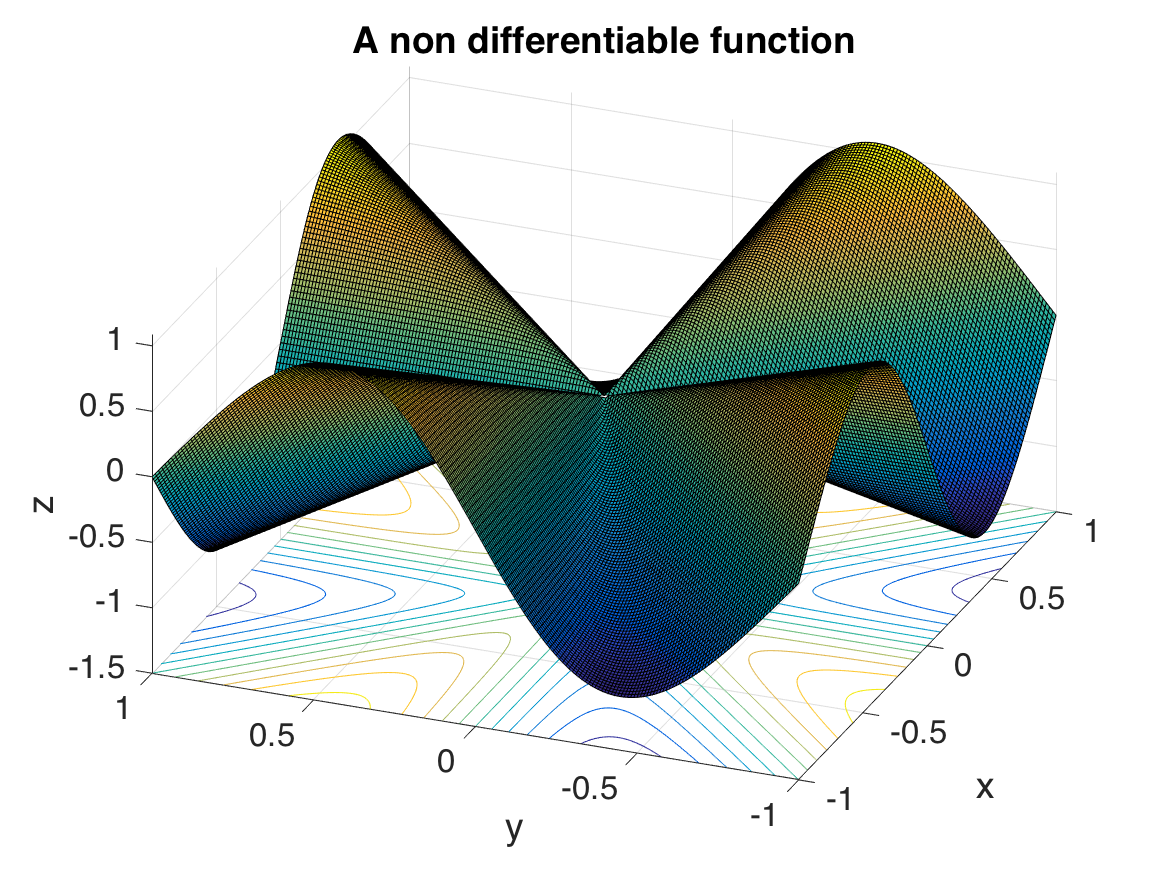
\includegraphics[width = 7cm]{paraumbloid.pdf}%
%\includegraphics[scale = 1]{eas_boar_1.pdf}%

\end{figure}


\subsection{Summary}

\begin{itemize}
\item
Like a tangent to a curve, we can use partial derivatives to find tangent planes to surfaces
\item
In 2 dimensions, partial derivatives can exist without there being a tangent plane
\item
so its always best to draw a picture
\end{itemize}


\subsection{The chain rule for partial differentiation}

\textbf{The chain rule: Case 1.}
Let $z=z(x,y)$. If $x=x(t)$, $y=y(t)$ is a curve in the $xy$-plane
traced out as the parameter $t$ varies, then $t \mapsto z=z(x(t), y(t))$ is a real valued function.
The chain rule gives
$$
\frac{dz}{dt} = \frac{\partial z}{\partial x} \frac{dx}{dt} + \frac{\partial z}{\partial y}\frac{dy}{dt}.
$$
The Chain Rule shows how to differentiate $z$ as a function of $t$ and is an immediate consequence of
$$
\Delta z = z_x \Delta x + z_y \Delta y = z_x \frac{dx}{dt} \Delta t + z_y \frac{dy}{dt} \Delta t
$$



\textbf{Example PD13.} If $f=x^2 y+ 3x y^4$ with $ x=\sin 2 t$ and $y= \cos t$,  find $dz/dt$ at $t=0$.
$$
\frac{dz}{dt} = \frac{\partial f}{\partial x} \frac{dx}{dt} +
\frac{\partial f}{\partial y}\frac{dy}{dt} = ( 2xy+ 3y^4)( 2 \cos
2t)+ (x^2+12 xy^3)(-\sin t).
$$
When $t=0$, we obtain $ dz/dt =6$.



\textbf{The Chain rule: Case 2}. Let $z=z(x,y)$ and suppose that
$x$ and $y$ are themselves functions of $s$ and $t$:
$$
x = x(s,t)\qquad y=y(s,t)
$$
How does this change of independent variable impact on partial derivatives?

We use a \textcolor{red}{chain rule} for several variables:
$$
\frac{\partial z}{\partial s} =
 \frac{\partial z}{\partial x} \frac{\partial x}{\partial s}
+ \frac{\partial z}{\partial y} \frac{\partial y}{\partial s}
$$
and
$$ \frac{\partial z}{\partial t} =
 \frac{\partial z}{\partial x} \frac{\partial x}{\partial t}
+ \frac{\partial z}{\partial y} \frac{\partial y}{\partial t}.
$$
These results can be used to generate second and higher order
derivatives, $z_{ss}$, $z_{st}$ and $z_{tt}$, etc., in terms of $x$ and
$y$ derivatives.



\textbf{Example PD14.} If $g(s, t)=f(s^2-t^2, t^2-s^2)$ and $f$ is
differentiable, show that $g$ satisfies
$$
t\frac{\partial g}{\partial s} + s \frac{\partial g}{\partial t}
=0.
$$
Let $ x=s^2-t^2, y=t^2-s^2$. Then
$$
\frac{\partial g}{\partial s} =
 \frac{\partial f}{\partial x} \frac{\partial x}{\partial s}
+ \frac{\partial f}{\partial y} \frac{\partial y}{\partial s}=2s\, f_x - 2s \, f_y
$$
$$
\frac{\partial g}{\partial t} =
 \frac{\partial f}{\partial x} \frac{\partial x}{\partial t}
+ \frac{\partial f}{\partial y} \frac{\partial y}{\partial t}=-2t \, f_x +2t \, f_y\,.
$$
Hence
$$
t\frac{\partial g}{\partial s} + s \frac{\partial g}{\partial t}
=0.
$$


\subsection{Summary}

\begin{itemize}
\item
As with usual functions of one variable, we can compute partial derivatives of functions of functions using a chain rule
\item
Similar to one variable case -- just need to keep a cool head
\end{itemize}


\section{Implicit differentiation}

Let $f=f(x,y)$ and suppose
\begin{equation}
\label{implicit}
f(x,y)=0\,.
\end{equation}
$x$ and $y$ such that this equation holds defines $y$ \textcolor{red}{implicitly} as a function of $x$, that is, $y=y(x)$.

Then the Chain Rule (Case 1) can be used: Differentiating both sides of (\ref{implicit}) 
with respect to $x$ gives
$$
 \frac{\partial f}{\partial x} \frac{d x}{d x}
+ \frac{\partial f}{\partial y} \frac{d y}{d x}=0 \; \to \;\;
\frac{dy}{dx} = - \frac{f_x}{f_y},
$$
since $\frac{dx}{dx}=1$. 


This can be generalised to the case where $z$ is given implicitly in terms of $x$ and $y$ through a relation of the form 
$$
f(x,y,z)=0.
$$
In this case we obtain
$$
 \frac{\partial f}{\partial x} \frac{\partial x}{\partial x}
+ \frac{\partial f}{\partial y} \frac{\partial y}{\partial x} +
\frac{\partial f}{\partial z} \frac{\partial z}{\partial x}=0\,.
$$
But $x$ and $y$ are independent variables so that
$$
 \frac{\partial y}{\partial x} =0 \quad \mbox{  whilst  } \quad \frac{\partial x}{\partial x}=1.
$$
Then, rearranging
$$
 \frac{\partial z}{\partial x} = - \frac{f_ x}{f_z}.
$$
Similar formulas work for other partial derivatives so that
$$
\frac{\partial z} {\partial y} = - \frac{f_y}{f_z}.
$$



\textbf{Example PD15.} Find $y'(x)$ at $(2,1)$ if 
$$ 
x^3+y^3=6xy-3. \quad \mbox{Here  } f (x,y) = x^3+y^3-6xy+3.
$$
$$
y'(x) = \frac{dy}{dx}=-\frac{f_x}{f_y}= -\frac{ 3x^2-6y}{3y^2-6x}\Big|_{(2,1)} = -\frac{6}{9}.
$$
\textbf{Example PD16.} Find $z_x$, $z_y$ and $z_{xy}$ if the equation
$$
 x+y-z=e^z
$$
is used to define $z$ as a function of the two independent variables $x$ and $y$.


Method I: Let $f(x,y,z)=x+y-z-e^z$.
$$
\frac{\pd f}{\pd x} = f_x = 1; \;\;\frac{\pd f}{\pd y} = f_y = 1;
\;\;\frac{\pd f}{\pd z} = f_z = -1-e^z.
$$
$$
 \frac{\partial z}{\partial x} = - \frac{f_ x}{f_z}= \frac{1 }{ 1+e^z}.
$$
By symmetry between $x$ and $y$:
$$
\frac{\partial z} {\partial y} = - \frac{f_y}{f_z}=\frac{1 }{
1+e^z}
$$
$$
\begin{array}{lll}
\frac{\pd^2 z }{\pd x \pd y} & = & \frac{\pd }{\pd y} \left( \frac{1
}{ 1+e^z} \right) = \frac{\pd }{\pd z} \left( \frac{1
}{ 1+e^z} \right) \frac{\pd z}{\pd y} =   -\frac{e^z}{ (1+e^z)^2} \;\frac{\partial z}
{\partial y}\\
\\
& = & -\frac{e^z}{ (1+e^z)^2} \; \frac{1 }{ 1+e^z} =-\frac{e^z }{ (1+e^z)^3}
\end{array}
$$


Method II: Differentiate both sides with respect to $x$:
$$
\frac{\pd}{\pd x}: x+y-z=e^z \;\; \to \;\; 1-\frac{\pd z}{\pd x}=e^z \frac{\pd z}{\pd
x};  \;\; \mbox{giving} \;\;  \frac{\partial z}{\partial x} = \frac{1 }{
1+e^z}. \hfill \textcolor{red}{( \dagger)}
$$
Differentiate both sides with respect to $y$:
$$
\frac{\pd}{\pd y}: x+y-z=e^z \;\; \to \;\; 1-\frac{\pd z}{\pd y}=e^z \frac{\pd z}{\pd
y};  \;\;  \mbox{giving}\;\;  \frac{\partial z}{\partial y} = \frac{1 }{
1+e^z}.
$$
Differentiate both sides of \textcolor{red}{$(\dagger)$} with respect to $y$
{
$$
\frac{\pd}{\pd y} \left( 1-\frac{\pd z}{\pd x} \right) = \frac{\pd}{\pd y} \left( e^z \frac{\pd z}{\pd
x} \right) \implies -\frac{\pd^2 z}{\pd x \pd y } =e^z \frac{\pd^2 z}{\pd x \pd y} +
 e^z \frac{\pd z}{\pd y}  \frac{\pd z}{\pd x}  .
$$
}
i.e.,
$$
\frac{\pd^2 z}{\pd x \pd y } = - \frac{e^z }{ 1+e^z} \;\frac{\pd
z}{\pd y}  \frac{\pd z}{\pd x}= -\frac{e^z }{ (1+e^z)^3}.
$$


\textbf{Example PD17.} Let
$$
z=u^v, \quad u=\sin x , \quad v=\cos x\,.
$$
Find $dz/dx$:
$$
\frac{d z}{d x} =\frac{\pd z}{\pd u} \frac{d u}{d x}+\frac{\pd
z}{\pd v} \frac{d v}{d x}
$$
where
$$
\frac{\pd z}{\pd u}=v u^{v-1}, \;\; \ln z = v \ln u \to \frac{1}{z} \frac{\pd z}{\pd v} = \ln u \to \frac{\pd z}{\pd v}= u^v \ln u
$$
which yields
$$
\begin{array}{lll}
\frac{d z}{d x} & = & \left( v u^{v-1} \right) \cos x - \left( u^v \ln u \right) \sin x \\
& = & (\sin x)^{\cos x -1}  \cos^2 x -   (\sin x)^{\cos x +1} \ln \sin x \\
& = & (\sin x)^{\cos x -1} \left( \cos^2 x - \sin^2 x \ln \sin x\right) .
\end{array}
$$


\textbf{Example PD18.}  Find $\partial z/\partial x$, $\partial
z/\partial y $  if the equation
$$
z=(x^2y+xy^2)^{\cos(xy)}
$$
defines $z$ as a function of the two independent variables $x$ and
$y$.\\

Note that
$$
\ln z=\cos(xy) \ln (x^2y+xy^2)
$$
Then
$$
\frac{1}{ z} \frac{\pd z}{\pd x} =-y \sin (xy) \ln (x^2y+xy^2)+
\cos(xy)  \;\;\frac{2xy+y^2}{x^2y+xy^2}
$$
$$
 \frac{\partial z}{\partial x} =  (x^2y+xy^2)^{\cos(xy)} \left[
-y \sin (xy) \ln (x^2y+xy^2)+ \cos(xy) \;\;\frac{2x+y}{x^2+xy}
\right]
$$


\subsection{Summary}

\begin{itemize}
\item
For functions of one variable related for example by $g(x, y(x)) = 0$, we can find $y' (x)$ by implicit differentiation.
\item we can do the same for functions of severable variables -- but here are many possibilities
\item
The approach can be powerful in finding deriviatives
\end{itemize}


\section{Simple Partial differential equations }

Partial differential equations (PDEs), like differential equations (ODEs), are
equations that involve \textcolor{red}{a to be found function} of several variables 
and its partial derivatives. 

This is best seen by simple examples.



\textbf{Example PD19.}:  The pde
$$
\frac{\partial u}{\partial x} =0
$$
for a function $u=u(x,y)$ simply states that $u$ does not depend on $x$. Its general solution is
therefore is
$$
u=w(y)
$$
where $w$ denotes an arbitrary function of $y$.


\textbf{Example PD20}: Find the general solution $u(x,y)$ so that
\begin{equation}\label{e1.2b}
\frac{\partial^2 u}{\partial x^2}= 0.
\end{equation}
Integrate with respect to $x$ to give
$$
\frac{\partial u}{\partial x}=f(y).
$$
Integrate with respect to $x$ again to give
$$
u(x,y)=f(y) x +g(y).
$$
Note that there are two arbitrary functions in the solution.


\textbf{Example PD21}: Find all $u(x,y)$ satisfying
\begin{equation}\label{e1.2b}
\frac{\partial^2 u}{\partial x \partial y}= 0.
\end{equation}
First, integrate it in $x$, regarding $y$ as fixed:
$$
\frac{\partial u}{\partial y}=f(y).
$$
Do it again to obtain
$$
u(x,y)=\int f(y) d y  +g(x),
$$
where both $f(y)$ and $g(x)$ are arbitrary functions. If we call the integral of $f(y)$ say $h(y)$ we get the most useful form:
$$
u(x,y)=g(x) + h(y) ,
$$
where both $g(x)$ and $h(y)$ are arbitrary functions.


\textbf{Example PD22} Find $a$ and $b$ in $\xi=x+ay, \eta=x+by$ such that they transform the equation
 $$
 6 \frac{\partial^2 u}{\partial x^2} +  \frac{\partial^2 u}{\partial x \partial y}
 - \frac{\partial^2 u}{\partial y^2} =0
$$
into
$$
 \frac{\partial^2 u }{\partial \xi \partial \eta} = 0.
$$
Hence, find the general solution of the PDE.

We have
$$
\xi_x=1, \quad \eta_x=1, \quad \xi_y=a, \quad \eta_y=b
$$
Then
{\small
$$
\begin{array}{lll}
\frac{\pd u}{\pd x}&=&\frac{\pd u}{\pd \xi}\frac{\pd \xi}{\pd
x}+\frac{\pd u}{\pd \eta}\frac{\pd \eta}{\pd x}=\frac{\pd u}{\pd
\xi} +\frac{\pd u}{\pd \eta} \\
\frac{\pd u}{\pd y}&=& \frac{\pd u}{\pd \xi}\frac{\pd \xi}{\pd
y}+\frac{\pd u}{\pd \eta}\frac{\pd \eta}{\pd y}=a\frac{\pd u}{\pd
\xi} + b\frac{\pd u}{\pd \eta}
\end{array}
$$
}


$$
\begin{array}{lll}
\frac{\pd^2 u}{\pd x^2}&=&\frac{\pd^2 u}{\pd \xi^2} + 2
\frac{\pd^2 u}{\pd \xi \pd \eta}+\frac{\pd^2 u}{\pd \eta^2} \\
\frac{\pd^2 u}{\pd y^2}&=& a^2 \frac{\pd^2 u}{\pd \xi^2} + 2ab
\frac{\pd^2 u}{\pd \xi \pd \eta}+ b^2 \frac{\pd^2 u}{\pd \eta^2} \\
\frac{\pd^2 u}{\pd x \pd y}&=& a \frac{\pd^2 u}{\pd \xi^2} + (a+b)
\frac{\pd^2 u}{\pd \xi \pd \eta}+ b \frac{\pd^2 u}{\pd \eta^2}
\end{array}
$$
It follows that
$$
6 \frac{\partial^2 u}{\partial x^2} +  \frac{\partial^2
u}{\partial x \partial y}
 - \frac{\partial^2 u}{\partial y^2}=0, \;\;  \to
$$
$$
( 6+ a-a^2) \frac{\pd^2 u}{\pd \xi^2} +( 12+a+b -2ab) \frac{\pd^2
u}{\pd \xi \pd \eta} + (6+b-b^2) \frac{\pd^2 u}{\pd \eta^2}= 0
$$
Now 
$$
6+ a-a^2 = 0 \mbox{ if } a = - 2 \mbox{ or } a = 3
$$
whilst 
$$
6+ b-b^2 = 0 \mbox{ if } b = - 2 \mbox{ or } b = 3
$$



Hence, if we choose $a = -2$ and $b = 3$, then independent $\xi=x-2y$ and $\eta=x+3y$ give
$$
25 \frac{\pd^2 u}{\pd \xi \pd \eta}= 0
$$
which has the general solution (as in a previous example) 
$$
u(x,y)=f(\xi) + g(\eta) = f( x - 2y)  +g(x +3 y)
$$
It is easy to check this:
$$
u_{xx} = f''(x-2y) + g''(x+3y), \quad
u_{xy} = -2 f''(x-2y) + 3 g''(x+3y)
$$
$$
u_{yy} = 4 f''(x-2y) + 9 g''(x+3y). 
$$
Substitution shows that the PDE is satisfied.



More generally, consider the linear PDE:
$$
q \frac{\partial^2 u}{\partial x^2} + p \frac{\partial^2 u}{\partial x \partial y} + \frac{\partial^2 u}{\partial y^2} =0, p^2 > 4q
$$
Following the approach above, with $\xi=x+ay, \eta=x+by$ we obtain:
{\small 
$$
\left( q + p a + a^2 \right) \frac{\pd^2 u}{\pd \xi^2} + \left( 2q + p (a + b) + 2ab \right) \frac{\pd^2
u}{\pd \xi \pd \eta} + \left( q + p b + b^2\right) \frac{\pd^2 u}{\pd \eta^2}= 0
$$
}
Choosing $a$ as one root of 
$$
m^2 + p m + q = 0
$$
and $b$ as the other gives $ab = q$ and $a+b = -p$ and so a simplified equation
$$
\left( 2q + p (a + b) + 2ab \right) \frac{\pd^2
u}{\pd \xi \pd \eta} = \left( 4q-p^2 \right)  \frac{\pd^2
u}{\pd \xi \pd \eta} = 0
$$
with solution $u = f(\xi) + g(\eta) = f(x+ay) + g(x+by)$.



\textbf{Example PD23.}  Find $z(x,y)$ if 
$$
z_{yy}=2x\mbox{   and    } z(x,1)=0, z_y(x,0)=\sin x.
$$
$$
\frac{\pd }{\pd y} \left( \frac{\pd z}{\pd y} \right) = 2x
$$
Integrating, we obtain
$$
 \frac{\partial z}{\partial y} =z_y(x,y)= 2xy+ \phi(x)
$$
Using the condition $ z_y(x,0)=\sin x$
$$
\sin x =0 + \phi(x)\quad\quad \mbox{i.e.}
$$
$$
 \frac{\partial z}{\partial y} = 2xy+ \sin x, \; \; \to \;\;
 z=xy^2 + y \sin x +\psi (x)
$$
$$
z(x,1)=0, \;\; \to \;\; 0 =x +  \sin x +\psi (x), \;\; \to \;\;
-(x +  \sin x ) =\psi (x),
$$
The function is $z(x,y)= xy^2 + y \sin x  -(x + \sin x )$.

\newpage

\subsection{Summary}

\begin{itemize}
\item
Partial differential equations (PDEs) is a huge topic - there is a final year module devoted to the topic.
\item
PDEs arise in numerous applications
\item
Here we have illustrated a few ideas and techniques
\end{itemize}

%
%\bigskip
%\centerline{KZ 4/1/2011}


\bigskip

\noindent{\bf Directional derivatives} In two dimensions, let $\bf
u$ be a unit vector, i.e $|{\bf u}| = 1.$ Then the directional
derivative, the rate of variation of $z = z(x,y)$ as we move in
the $\bf u$ direction is
$$
D_{\bf u} z = a \frac{\partial z} {\partial x} +
b \frac{\partial z} {\partial y},
$$
where ${\bf u} = (a,b)$. In three dimensions this generalises to
$f=f(x,y,z)$ giving
$$ D_{\bf u} f = a \frac{\partial f} {\partial x} +
b \frac{\partial f} {\partial y} + c \frac{\partial f} {\partial
z} ,$$ where the three-dimensional unit vector ${\bf u} =
(a,b,c).$


\bigskip

\noindent{\bf Gradient vectors, tangents and normals}. In two
dimensions we define the gradient vector,
$$
\nabla f \equiv \Bigr( \frac{\partial f} {\partial x},
\frac{\partial f} {\partial y} \Bigr),
$$
and the directional
derivative formula can then be written as a scalar product
$$
D_{\bf u} f = {\bf u} \cdot \nabla f.
$$
The magnitude of the
directional derivative is then greatest when $\bf u$ is parallel
to $\nabla f$, which means that $\nabla f$ is the direction of
steepest ascent, interpreting $z=f(x,y)$ as height above the
$xy$-plane. Level contours are perpendicular to $\nabla f$.

In three dimensions,
$$
\nabla f \equiv \Bigr(\frac{\partial f} {\partial x},
\frac{\partial f} {\partial y}, \frac{\partial f} {\partial z}
\Bigr).
$$
$f(x,y,z)=C=$ const. is then a level surface. $\nabla
f$ is then a vector in the direction of the normal to this level
surface, i.e. perpendicular to the tangent plane at the surface.
For all unit vectors with their foot at the point $P =
(x_0,y_0,z_0)$ and lying in the tangent plane, ${\bf u} \cdot
\nabla f = 0$. The equation of the tangent plane through $P$ is
$$
(x-x_0) \frac{\partial f} {\partial x}
+(y-y_0) \frac{\partial f} {\partial y} + (z-z_0) \frac{\partial
f} {\partial z}=0,
$$
the partial derivatives being evaluated at $P$.







\begin{enumerate}

\item[3(A)] Representing and visualising functions of 2 variables.

\begin{enumerate}

\item[(i)] $z=f(x,y)$ is the height above the $xy$-plane, or
the depth below if $z$ is negative.

\item[(ii)] Functions can be drawn as perspective plots
(almost always done using a package such as MAPLE), or as
a contour plot. Contour plots are sketches of the level curves
$f(x,y) = z = $ const. in the $xy$-plane. Contour maps such as
the Ordnance Survey maps are examples of functions of height
in terms of $x$ and $y$ coordinates (the grid reference).

\item[(iii)] $z = c - x^2 -y^2$ has a local minimum at $x = y =0$.
Its contours are circles centred on the origin. $z = c+x^2+y^2$
has a local maximum at $x=y=0$. $z=x^2-y^2$ also is locally
flat at $x=y=0$, but it has a saddle point there. A saddle
is like a pass going from one valley to another, between two
mountains.

\end{enumerate}

\item[3(B)] Partial derivatives.

\begin{enumerate}

\item[(i)] If $z=z(x,y)$, ${ds \frac{\partial z}{\partial x}}$
means differentiate $z$ with respect to $x$ treating $y$ as a constant.
Similarly   ${ds \frac{\partial z}{\partial y}}$ means differentiate
$z$ with respect to $y$ treating $x$ as a constant.

\item[(ii)] Geometrical interpretation: ${ds \frac{\partial z}{\partial x}}$
is the tangent of the uphill or downhill slope of $z$ as we move in
the $x$ direction holding $y$ constant. Similarly,
${ds \frac{\partial z}{\partial y}}$ is the slope $z$ against $y$
with $x$ held constant.

\item[(iii)] Higher derivatives: ${ds \frac{\partial^2 z}{\partial x^2}}$
means ${ds \frac{\partial} {\partial x}
\Bigl( \frac{\partial z}{\partial x} \Bigr) }$. Similarly
${ds \frac{\partial^2 z}{\partial y^2}}$ means
${ds \frac{\partial} {\partial y}
\Bigl( \frac{\partial z}{\partial y} \Bigr) }$. The mixed
derivative,
$${ds \frac{\partial^2 z}{\partial x \partial y} =
 \frac{\partial} {\partial x}
\Bigl( \frac{\partial z}{\partial y} \Bigr)
= \frac{\partial} {\partial y}
\Bigl( \frac{\partial z}{\partial x} \Bigr)=
\frac{\partial^2 z}{\partial y \partial x} }.$$

\item[(iv)] Notation: $f_x$ means ${ds \frac{\partial f}{\partial x}}$,
${ds f_{xx} \equiv \frac{\partial^2 f}{\partial x^2}}$,
${ds f_{xy} = f_{yx} \equiv \frac{\partial^2 f}{\partial x \partial y}}$,
etc.

\end{enumerate}

\item[3(C)]  Linearisation and the tangent plane.

If $z= z(x,y)$ then
  $$ dz = \frac{\partial z}{\partial x} dx +
\frac{\partial z}{\partial y} dy .$$
The tangent plane to the surface $z = z(x,y)$ at the point $ P=$
$(x_0, y_0, z_0)$ is
$$ds { z-z_0 = (x-x_0) \frac{\partial z}{\partial x}
+ (y-y_0) \frac{\partial z}{\partial y} }.$$
This tangent plane
formula is also called the linearisation of $z=z(x,y)$ about
the point $P$.
See (3H) below for
the case where the surface is given implicitly, i.e. $f(x,y,z)=0$.

\item[3(D)]  Total derivatives and the chain rule.

If $z=z(x,y)$ and $x=x(t)$, $y=y(t)$ is a curve in the $xy$-plane
traced out as the parameter $t$ varies, then the chain rule is
$$ \frac{dz}{dt} = \frac{\partial z}{\partial x}
\frac{dx}{dt} + \frac{\partial z}{\partial y}\frac{dy}{dt}.$$
Note that if there is a relation between $x$ and $y$, then
$ds { \frac{dz}{dx} = \frac{\partial z}{\partial x}
+ \frac{\partial z}{\partial y} \frac{dy}{dx} }$, so the
partial derivative is not the same as the total derivative.

\item[3(E)]  Chain rule for functions of several variables.

Given $z=z(x,y)$ and we want to change independent variables from $x$ and $y$
to $s$ and $t$, and we are given $x=x(s,t)$ and $y=y(s,t)$. There
are formulae for finding ${ds \frac{\partial z}{\partial s}}$ in terms
of ${ds \frac{\partial z}{\partial x}}$ and
${ds \frac{\partial z}{\partial y}}$. These are the chain rules for
several variables,
$$ \frac{\partial z}{\partial s} =
 \frac{\partial z}{\partial x} \frac{\partial x}{\partial s}
+ \frac{\partial z}{\partial y} \frac{\partial y}{\partial s}$$
and
$$ \frac{\partial z}{\partial t} =
 \frac{\partial z}{\partial x} \frac{\partial x}{\partial t}
+ \frac{\partial z}{\partial y} \frac{\partial y}{\partial t}.$$
These results can be used to generate the second order derivatives,
$z_{ss}$, $z_{st}$ and $z_{tt}$ in terms of $x$ and $y$ derivatives.

\item[3(F)]  Implicit differentiation.

If $f(x,y)=0$, then ${ds \frac{dy}{dx} = - \frac{f_x}{f_y} }$. This
can be generalised to the case where $z$ is given implicitly in terms
of $x$ and $y$ through a relation of the form $f(x,y,z)=0$.
Then
$$df = f_x dx + f_y dy + f_z dz =0$$
can be used to find the partial derivatives, e.g.
$$ \frac{\partial z} {\partial x} = - \frac{f_x}{f_z}$$
since $dy=0$ when finding the partial derivative of $z$ with
respect to $x$. Similar formula work for other partial derivatives,
and since $x$,$y$ and $z$ appear symmetrically in $f(x,y,z)=0$
we can also write
$$ \frac{\partial x} {\partial y} = - \frac{f_y}{f_x}$$
where now the partial derivative of $x$ with respect to $y$
means that $z$ is held constant $( dz =0)$.

\item[3(G)]  Directional derivatives.

In two dimensions, let $\bf u$ be a unit vector, i.e $|{\bf u}| = 1.$
Then the directional derivative, the rate of variation of $z = z(x,y)$
as we move in the $\bf u$ direction is
$$ D_{\bf u} z = a \frac{\partial z} {\partial x} +
b \frac{\partial z} {\partial y},$$
where ${\bf u} = (a,b)$. In three dimensions this generalises to
$f=f(x,y,z)$ giving
$$ D_{\bf u} f = a \frac{\partial f} {\partial x} +
b \frac{\partial f} {\partial y} + c \frac{\partial f} {\partial z} ,$$
where the three-dimensional unit vector ${\bf u} = (a,b,c).$

\item[3(H)]  Gradient vectors, tangents and normals.

In two dimensions we define the gradient vector,
$$ \nabla f \equiv \Bigr( \frac{\partial f} {\partial x},
\frac{\partial f} {\partial y} \Bigr), $$
and the directional derivative formula can then be written
as a scalar product
${ds D_{\bf u} f = {\bf u} \cdot \nabla f }.$ The magnitude
of the directional derivative is then greatest when $\bf u$
is parallel to $\nabla f$, which means that $\nabla f$ is
the direction of steepest ascent, interpreting $z=f(x,y)$ as
height above the $xy$-plane. Level contours are perpendicular
to $\nabla f$.

In three dimensions,
$$ \nabla f \equiv \Bigr(\frac{\partial f} {\partial x},
\frac{\partial f} {\partial y}, \frac{\partial f} {\partial z} \Bigr). $$
$f(x,y,z)=C=$ const. is then a level surface. $\nabla f$ is then
a vector in the direction of the normal to this level surface, i.e.
perpendicular to the tangent plane at the surface. For all unit
vectors with their foot at the point $P = (x_0,y_0,z_0)$ and
lying in the tangent plane, ${\bf u} \cdot \nabla f = 0$.
The equation of the tangent plane through $P$ is
$$ (x-x_0) \frac{\partial f} {\partial x}
+(y-y_0) \frac{\partial f} {\partial y}
+ (z-z_0) \frac{\partial f} {\partial z}=0, $$
the partial derivatives being evaluated at $P$.
\end{enumerate}

\section{Gradient Vectors and Directional Derivatives}
\subsection{Directional derivatives}

In two dimensions, let $\bf u$ be a unit vector, i.e
$$
{\bf u}=a{\bf i} + b {\bf j}=(a,b); \;\; |{\bf u}| = \sqrt{a^2 +b^2} = 1.
$$
Then the directional derivative, the rate of variation of $z =
f(x,y)$ as we move in the $\bf u$ direction, is
$$
D_{\bf u} f = a \frac{\partial z} {\partial x} + b \frac{\partial
z} {\partial y}.
$$
In three dimensions this generalises to $f=f(x,y,z)$ giving
$$ D_{\bf u} f = a \frac{\partial f} {\partial x} +
b \frac{\partial f} {\partial y} + c \frac{\partial f} {\partial
z} ,$$ where the three-dimensional unit vector ${\bf u} =
(a,b,c).$

\subsection{2-D Gradient vectors}

In two dimensions we define the gradient vector, or ``nabla'', as
$$
\nabla f \equiv \Bigr( \frac{\partial f} {\partial x},
\frac{\partial f} {\partial y} \Bigr),
$$
and the directional derivative formula can then be written as a
scalar product
$$
D_{\bf u} f = {\bf u} \cdot \nabla f.
$$
\vspace{-.5cm}

\begin{itemize}
\item
The magnitude of the directional derivative is greatest when
$\bf u$ is parallel to $\nabla f$;
\item
$\nabla f$ is the direction of steepest ascent, interpreting $z=f(x,y)$ as
height above the $xy$-plane;
\item
$\nabla f$ is perpendicular, i.e. normal, to the 
level contours of $f$\,.
\end{itemize}
The latter is a consequence of 
$$
f(x,y) = \mbox{ constant  } \to y = y(x) \mbox{ and } \frac{dy}{dx} = - \frac{f_x}{f_y}
$$
Tangent: direction $= (f_y, -f_x)$; So normal has direction \textcolor{red}{$(f_x, f_y)$}.



\textbf{Example}. Find the directional derivative of
$f=x^2y^3-4y$ at the point $(2,-1)$ in the direction of ${\bf v} =
2{\bf i}+ 5{\bf j}$. \\

We first compute the gradient vector
$$
\nabla f (x,y) = \frac{\partial f} {\partial x} {\bf i}+
\frac{\partial f} {\partial y} {\bf j}=2xy^3 {\bf
i}+(3x^2y^2-4){\bf j},
$$
Then
$$
\nabla f_{(2,-1)} = -4 {\bf i}+8{\bf j}.
$$
We then find the unit vector in the direction of ${\bf v}$
$$
{\bf u} = \frac{\bf v} {|{\bf v}|}= \frac{2}{\sqrt{29}}{\bf i} +
 \frac{5}{\sqrt{29}} {\bf j}.
$$
Finally, we work out the scalar product
$$
D_{\bf u} f = {\bf u} \cdot \nabla f=\left[
\frac{2}{\sqrt{29}}{\bf i} +
 \frac{5}{\sqrt{29}} {\bf j} \right] \cdot \left[ -4 {\bf i}+8{\bf j}
 \right]=
\frac{-8+40}{\sqrt{29}}
$$


\subsection{3-D Gradient vectors}

In three dimensions,
$$
\nabla f \equiv \Bigr(\frac{\partial f} {\partial x},
\frac{\partial f} {\partial y}, \frac{\partial f} {\partial z}
\Bigr).
$$
\begin{itemize}
\item
$f(x,y,z)=C=$ const. is then a level surface. 
\item
$\nabla f$ is then a
vector in the direction of the normal to this level surface, i.e.
perpendicular to the tangent plane at the surface. 
\item
The directional derivative formula can then be written as a scalar product
$$
D_{\bf u} f(x,y,z) = {\bf u} \cdot \nabla f.
$$
\end{itemize}

\subsection{Tangent Plane to a Surface} 

Let $S$ be the surface $f(x,y,z)=k$, i.e. a level surface of $f$.

The \textbf{tangent plane} to $S$ at $P = (x_0,y_0,z_0)$ 
has normal vector $ \nabla f$ evaluated at $P$.

Hence the \textcolor{red}{TANGENT PLANE} has equation
$$
\left[ {\bf r}-{\bf r}_0 \right] \cdot \nabla f_{(x_0,y_0,z_0)}=0
$$
where ${\bf r}$ is the position vector of a point $(x,y,z)$. 

Equivalently,
$$
(x-x_0) \frac{\partial f} {\partial x} +(y-y_0) \frac{\partial f}
{\partial y} + (z-z_0) \frac{\partial f} {\partial z}=0\,.
$$

\subsection{Normal Line to a Surface} 

The \textbf{Normal line} to the surface $S$ at the point $P$ is the line perpendicular
(i.e. orthogonal) to the tangent plane

The direction of the normal line is therefore given by the gradient
vector $\nabla F$ evaluated at $P$. 

Hence, the \textcolor{red}{NORMAL LINE} can be written as
$$
{\bf r}- {\bf r}_0 = t (\nabla f)_{(x_0,y_0,z_0)},
$$
where $t$ is a parameter. 

In $(x, y, z)$ coordinates this is
$$
\frac{(x-x_0)}{f_x{(x_0,y_0,z_0)}} =
\frac{(y-y_0)}{f_y{(x_0,y_0,z_0)}}=\frac{(z-z_0)}{f_z{(x_0,y_0,z_0)}}.
$$



\textbf{Example}. Find the equation of the tangent plane and
normal line at the point  $(-2,1,-3)$ to the ellipsoid
$$
\frac{x^2}{4}+ y^2+\frac{z^2}{9}=3.
$$
The ellipsoid is the level surface $f = 3$ of the function
$$
f (x,y,z) =\frac{x^2}{4}+ y^2+\frac{z^2}{9}
$$
We have $f_x=x/2, \;\; f_y=2y, \;\; f_z=2z/9$ so that
$$
f_x{(-2,1,-3)}=\textcolor{red}{-1}; \quad f_y{(-2,1,-3)}=\textcolor{red}{2}; \quad f_z{(-2,1,-3)}=\textcolor{red}{-2/3}.
$$
The tangent plane is therefore
$$
(x+2)\textcolor{red}{(-1)}+(y-1)\textcolor{red}{2}+ (z+3)\textcolor{red}{(-2/3)}=0\;\; \to \;\; 3x-6y+2z+18=0.
$$
The normal line is
$$
 \frac{x+2}{\textcolor{red}{-1}} = \frac{y-1}{\textcolor{red}{2}} =\frac{z+3}{\textcolor{red}{-2/3}}.
$$


\section{Summary}

\begin{itemize}
\item
The gradient of a function $f(x,y)$ (in 2D) of $f(x,y,z)$ in 3D, or ``nabla'' is the vector of partial derivatives
$$
\nabla f = (f_x, f_y) \qquad \mbox{or} \qquad (f_x, f_y, f_z)
$$
\item
The directional derivative ${\bf u} \cdot \nabla f$ tells us the rate of increase of $f$ in the direction of ${\bf u}$.
\item
We can use $\nabla f$ to find the tangent planes and normal lines to a surface $f(x,y,z) = $ constant, at a point $P = (x_0, y_0, z_0)$, via
$$
\underbrace{(x, y, z) = (x_0, y_0, z_0) + t \nabla f_P}_{\mbox{Normal line}} \qquad 
\underbrace{(x-x_0, y-y_0, z-z_0) \cdot \nabla f_P = 0}_{\mbox{Tangent Plane}}
$$
\end{itemize}


%\end{document}
\section{Multivariable Taylor Series}

\textcolor{red}{Taylor series in two variables.} Let $f(x,y)$ have
continuous partial derivatives. 

Recall the usual Taylor Series formula near the point $t=c$ of a scalar function $t \mapsto F(t)$:
$$
F(t)=F(c)+F'(c)(t-c)+\frac{1}{2!} (t-c)^2 F''(c)+ \ldots + \frac{1}{n!} (t-c)^n F^n(c)....
$$
Let $h$ and $k$ be sufficiently small and set
$$
x=a+t h, \;\; y=b+tk, \;\;  0 \le t \le 1.
$$
Define $F(t)=f(a+th, b+tk)$. Then the \textcolor{red}{CHAIN RULE} gives
$$
F'(t)=\frac{\partial f}{\partial x} \frac{d x}{d t} + \frac{\partial f}{\partial y} \frac{d y}{d t}=\frac{\partial f}{\partial x} h + \frac{\partial f}{\partial y} k
$$
$$
\begin{array}{lll}
F''(t) & = & \frac{\partial F'}{\partial x} \frac{d x}{d t} + \frac{\partial F'}{\partial y} \frac{d y}{d t} = \frac{\partial}{\partial x} \left( hf_x+kf_y \right) h + \frac{\partial}{\partial y}\left( hf_x+kf_y \right) k\\
& = & h^2 f_{xx}+ 2hk
f_{xy}+k^2f_{yy}.
\end{array}
$$


Applying Taylor's formula at $c=0$
{\small
$$
F(t)=F(0)+F'(0)(t-0)+\frac{1}{2} (t-0)^2 F''(0)+ \ldots
$$
}
and setting $t=1$, so that \textcolor{red}{$x = a + h$ and $y = b + k$}, gives
{\small
$$
F(1)=F(0)+F'(0)(1-0)+\frac{1}{2} (1-0)^2 F''(0)+....
$$
}
In terms of $f(a + th, b+tk)$ with $t=1$ this becomes
{\small
$$
\begin{array}{lll}
f(a+h,b+k) & = & f(a,b)+\left( h \frac{\partial f}{\partial x} + k
\frac{\partial f}{\partial y}  \right)_{(a,b)} + \\
& & \frac{1}{2!} \left( h^2 \frac{\partial^2
f}{\partial x^2} + 2hk \frac{\partial^2 f}{\partial x \partial y}
+ k^2 \frac{\partial^2 f}{\partial y^2}\right)_{(a,b)} + \ldots
\end{array}
$$
}
{\small
$$
\hspace{-.5cm}
= \textcolor{red}{f(a,b)} + \textcolor{red}{\left[ \frac{\partial f}{\partial x}, 
\frac{\partial f}{\partial y} \right]_{(a,b)}} \left( \begin{array}{c} h\\k \end{array} \right) + \frac{1}{2} \left( \begin{array}{c} h\\k \end{array} \right)^T \textcolor{red}{\left[ \begin{array}{cc}
\frac{\partial ^2 f}{\partial x ^2} & \frac{\partial ^2 f}{\partial x \partial y}\\\frac{\partial ^2 f}{\partial x \partial y} & \frac{\partial ^2 f}{\partial y ^2} \end{array} \right]_{(a,b)} }\left( \begin{array}{c} h\\k \end{array} \right) + \ldots 
$$
}

\subsection{Linear Approximation and Hessian}

It follows that close to $(a,b)$ we can approximate $f(x,y)=f(a+h,b+k)$ quite well by the quadratic function
{\small
$$
\hspace{-.5cm}
\textcolor{red}{f(a,b)} + \textcolor{red}{\left[ \frac{\partial f}{\partial x}, 
\frac{\partial f}{\partial y} \right]_{(a,b)}} \left( \begin{array}{c} h\\k \end{array} \right) + \frac{1}{2} \left( \begin{array}{c} h\\k \end{array} \right)^T \textcolor{red}{\left[ \begin{array}{cc}
\frac{\partial ^2 f}{\partial x ^2} & \frac{\partial ^2 f}{\partial x \partial y}\\\frac{\partial ^2 f}{\partial x \partial y} & \frac{\partial ^2 f}{\partial y ^2} \end{array} \right]_{(a,b)} }\left( \begin{array}{c} h\\k \end{array} \right) + \ldots 
$$
}
determined by
\begin{itemize}
\item
the \textcolor{red}{value} of $f$, i.e. $f(a,b)$ \qquad \textcolor{red}{CONSTANT PART}
\item
the \textcolor{red}{linearisation} of $f(x,y)$ near to $(a,b,)$
$$
\nabla f_{(a,b)} \equiv \Bigr( \frac{\partial f} {\partial x},
\frac{\partial f} {\partial y} \Bigr)_{(a,b)} \qquad \mbox{\textcolor{red}{LINEAR PART}}
$$
\item
the \textcolor{red}{Hessian} at $(a,b)$
$$
\left[ \begin{array}{cc}
\frac{\partial ^2 f}{\partial x ^2} & \frac{\partial ^2 f}{\partial x \partial y}\\\frac{\partial ^2 f}{\partial x \partial y} & \frac{\partial ^2 f}{\partial y ^2} \end{array} \right]_{(a,b)} 
\qquad \mbox{\textcolor{red}{QUADRATIC PART}}
$$
\end{itemize}
%We will use this quadratic approximation to find local \textcolor{red}{maxima} and \textcolor{red}{minima} of multivariable functions.

%\end{document}
%Since the Taylor series involves powers of $h$ and $k$, it
%converges rapidly when $h$ and $k$ are small, so it gives a good
%approximation to the behaviour of $f$ in the immediate
%neighbourhood of $(a,b)$.
%Return back to the variables $(x,y)$ 
%$$
%x=a+h, \;\; y= b+k,
%$$
%the Taylor series for two variables at the Point $(a,b)$ is
%$$
%f(x,y)=f(a,b)+  \left[ (x-a)\frac{\partial f}{\partial x} + (y-b)
%\frac{\partial f}{\partial y}  \right]_{a,b} + \frac{1}{2!} \left[ (x-a)^2 \frac{\partial^2
%f}{\partial x^2} + 2(x-a)(y-b)\frac{\partial^2 f}{\partial x \partial y}
%+ (y-b)^2 \frac{\partial^2 f}{\partial y^2}\right]_{a,b} + \cdots,
%$$
%where we have assumed that partial derivatives are continuous.
%
%
%If the two variable Taylor series formula is truncated at
%$$
%f(a+h,b+k)=f(a,b)+h \frac{\partial f}{\partial x} + k
%\frac{\partial f}{\partial y} + \cdots
%$$
%this is called the linear approximation of $f(x,y)$ about $(a,b)$,
%where $x=a+h$ and $y=b+k$, i.e.,
%$$
%f(x, y) \approx f(a,b)+(x-a) \frac{\partial f}{\partial x}(a,b) +
%(y-b) \frac{\partial f}{\partial y}(a,b).
%$$
%
%
%\bigskip


Applications of the formula
{\small
$$
\hspace{-.5cm}
\textcolor{red}{f(a,b)} + \textcolor{red}{\left[ \frac{\partial f}{\partial x}, 
\frac{\partial f}{\partial y} \right]_{(a,b)}} \left( \begin{array}{c} h\\k \end{array} \right) + \frac{1}{2} \left( \begin{array}{c} h\\k \end{array} \right)^T \textcolor{red}{\left[ \begin{array}{cc}
\frac{\partial ^2 f}{\partial x ^2} & \frac{\partial ^2 f}{\partial x \partial y}\\\frac{\partial ^2 f}{\partial x \partial y} & \frac{\partial ^2 f}{\partial y ^2} \end{array} \right]_{(a,b)} }\left( \begin{array}{c} h\\k \end{array} \right) + \ldots 
$$
}

\textbf{Example}. Find the linear approximation to
$$
f(x,y)=2x^2+y^2
$$
at the point $(1,1)$. Here $f(1,1) = 3$, $f_x = 4x, f_y = 2y$ so that $\nabla f_{(1,1)} =[4 \,\, 2]$ giving a linear approximation
$$
f (x,y) \approx 3+ 4(x-1)+ 2(y-1)=4x+2y-3,
$$
of $f$ at the point $(1,1)$.


\textbf{Example}.  Find the Taylor series  for
$$
f(x,y) = e^x \ln(1+y)
$$
about the point $a=0$, $b=0$ in powers of $h$ and $k$, where $x=h$ and $y=k$, up to and including the
quadratic terms.
{\small
$$
\hspace{-.1cm}
f\approx \textcolor{red}{f(0,0)} + \textcolor{red}{\left[ \frac{\partial f}{\partial x}, 
\frac{\partial f}{\partial y} \right]_{(0,0)}} \left( \begin{array}{c} h\\k \end{array} \right) + \frac{1}{2} \left( \begin{array}{c} h\\k \end{array} \right)^T \textcolor{red}{\left[ \begin{array}{cc}
\frac{\partial ^2 f}{\partial x ^2} & \frac{\partial ^2 f}{\partial x \partial y}\\\frac{\partial ^2 f}{\partial x \partial y} & \frac{\partial ^2 f}{\partial y ^2} \end{array} \right]_{(0,0)} }\left( \begin{array}{c} h\\k \end{array} \right) + \ldots 
$$
}
Here: $f_x = e^x \ln(1+y), \quad f_y = e^x/(1+y)$ and
$$
\quad f_{xx} = e^x \ln(1+y) \quad f_{xy}=e^x/(1+y) \quad f_{yy} = {-e^x/(1+y)^2}
$$
So
{\small
$$
f(0,0) = 0, \quad \nabla f_{(a,b)} =[0\,\,1] \qquad \left[ \begin{array}{cc}
\frac{\partial ^2 f}{\partial x ^2} & \frac{\partial ^2 f}{\partial x \partial y}\\\frac{\partial ^2 f}{\partial x \partial y} & \frac{\partial ^2 f}{\partial y ^2} \end{array} \right]_{(a,b)} =
\left[ \begin{array}{cc}
0 & 1\\1 & -1 \end{array} \right]
$$
}
and therefore
{\small
$$
f(h,k) \approx 0+ 0 \times h + k \times 1 + \frac{1}{2!} \left( h^2 \times 0 + 2hk \times 1  + k^2 \times (-1)\right)  = k+ hk-k^2/2
$$
}


\textbf{Matlab Example}.  Find the Taylor series expansion for
$f(x,y) = \sin x \sin y $ about the point $a=\frac{\pi}{4}$, $b=\frac{\pi}{4}$
in powers of $h$ and $k$, where $x=\frac{\pi}{4}+h$ and $y=\frac{\pi}{4}+k$, up to
and including the quadratic terms.
{\small 
$$
f_x = \cos x \sin y, \qquad f_y = \sin x \cos y
$$
}
{\small
$$
f_{xx} =-\sin x \sin y,\qquad f_{xy} = \cos x \cos y\qquad
f_{yy}=-\sin x \sin y.
$$
}
Evaluated at $(0,0)$ this leads to
$$
f(\frac{\pi}{4}+h,\frac{\pi}{4}+k)\approx 1/2 + \frac{1}{2} h +
\frac{1}{2}k + \frac{1}{2!} \left( -\frac{1}{2} h^2  + hk  -
\frac{1}{2} k^2 \right),
$$
or, in terms of $x$ and $y$,
{\small
$$
\frac{1}{2} + \frac{1}{2} (x-\frac{\pi}{4}) +
\frac{1}{2}(y-\frac{\pi}{4}) + \frac{1}{2!} \left[ -\frac{1}{2} (x-\frac{\pi}{4})^2  + (x-\frac{\pi}{4})(y-\frac{\pi}{4})  -
\frac{1}{2} (y-\frac{\pi}{4})^2 \right].
$$
}


\textbf{Matlab Example}.  Find the Taylor series expansion for
{\small
$$
f(x,y) = \sin x \sin y
$$ 
}
about the point $a=\frac{\pi}{4}$, $b=\frac{\pi}{4}$
in powers of $h$ and $k$, where $x=\frac{\pi}{4}+h$ and $y=\frac{\pi}{4}+k$, up to
and including the quadratic terms.
{\small 
$$
f_x = \overbrace{\cos x \sin y}^{\frac{1}{2}}, \qquad f_y = \overbrace{\sin x \cos y}^{\frac{1}{2}}
$$
}
{\small
$$
f_{xx} =\overbrace{-\sin x \sin y}^{-\frac{1}{2}},\qquad f_{xy} = \overbrace{\cos x \cos y}^{\frac{1}{2}}\qquad
f_{yy}=\overbrace{-\sin x \sin y}^{-\frac{1}{2}}.
$$
}
Evaluated at $(0,0)$ this leads to
{\small
$$
f(\frac{\pi}{4}+h,\frac{\pi}{4}+k)\approx 1/2 + \frac{1}{2} h +
\frac{1}{2}k + \frac{1}{2!} \left( -\frac{1}{2} h^2  + hk  -
\frac{1}{2} k^2 \right),
$$
}
or, in terms of $x$ and $y$,
{\small
$$
\frac{1}{2} + \frac{1}{2} (x-\frac{\pi}{4}) +
\frac{1}{2}(y-\frac{\pi}{4}) + \frac{1}{2!} \left[ -\frac{1}{2} (x-\frac{\pi}{4})^2  + (x-\frac{\pi}{4})(y-\frac{\pi}{4})  -
\frac{1}{2} (y-\frac{\pi}{4})^2 \right].
$$
}


\subsection{Local behaviour of multivariable functions}

\begin{figure}[!ht]
\vspace{-.2cm}
\centering
\includegraphics[width = 0.3\textwidth]{Contour_plot_min_saddle.pdf}%
%\includegraphics[scale = 1]{eas_boar_1.pdf}%
\caption{Contour plot of the function $f(x,y)=5x^2-\frac{x^3}{3}+8y^2-3x^2y$}
%\label{PP_sim1}%
\end{figure}


$$
f(x,y)=5x^2-\frac{x^3}{3}+8y^2-3x^2y
$$
\begin{figure}[!ht]
\vspace{-.5cm}
\centering
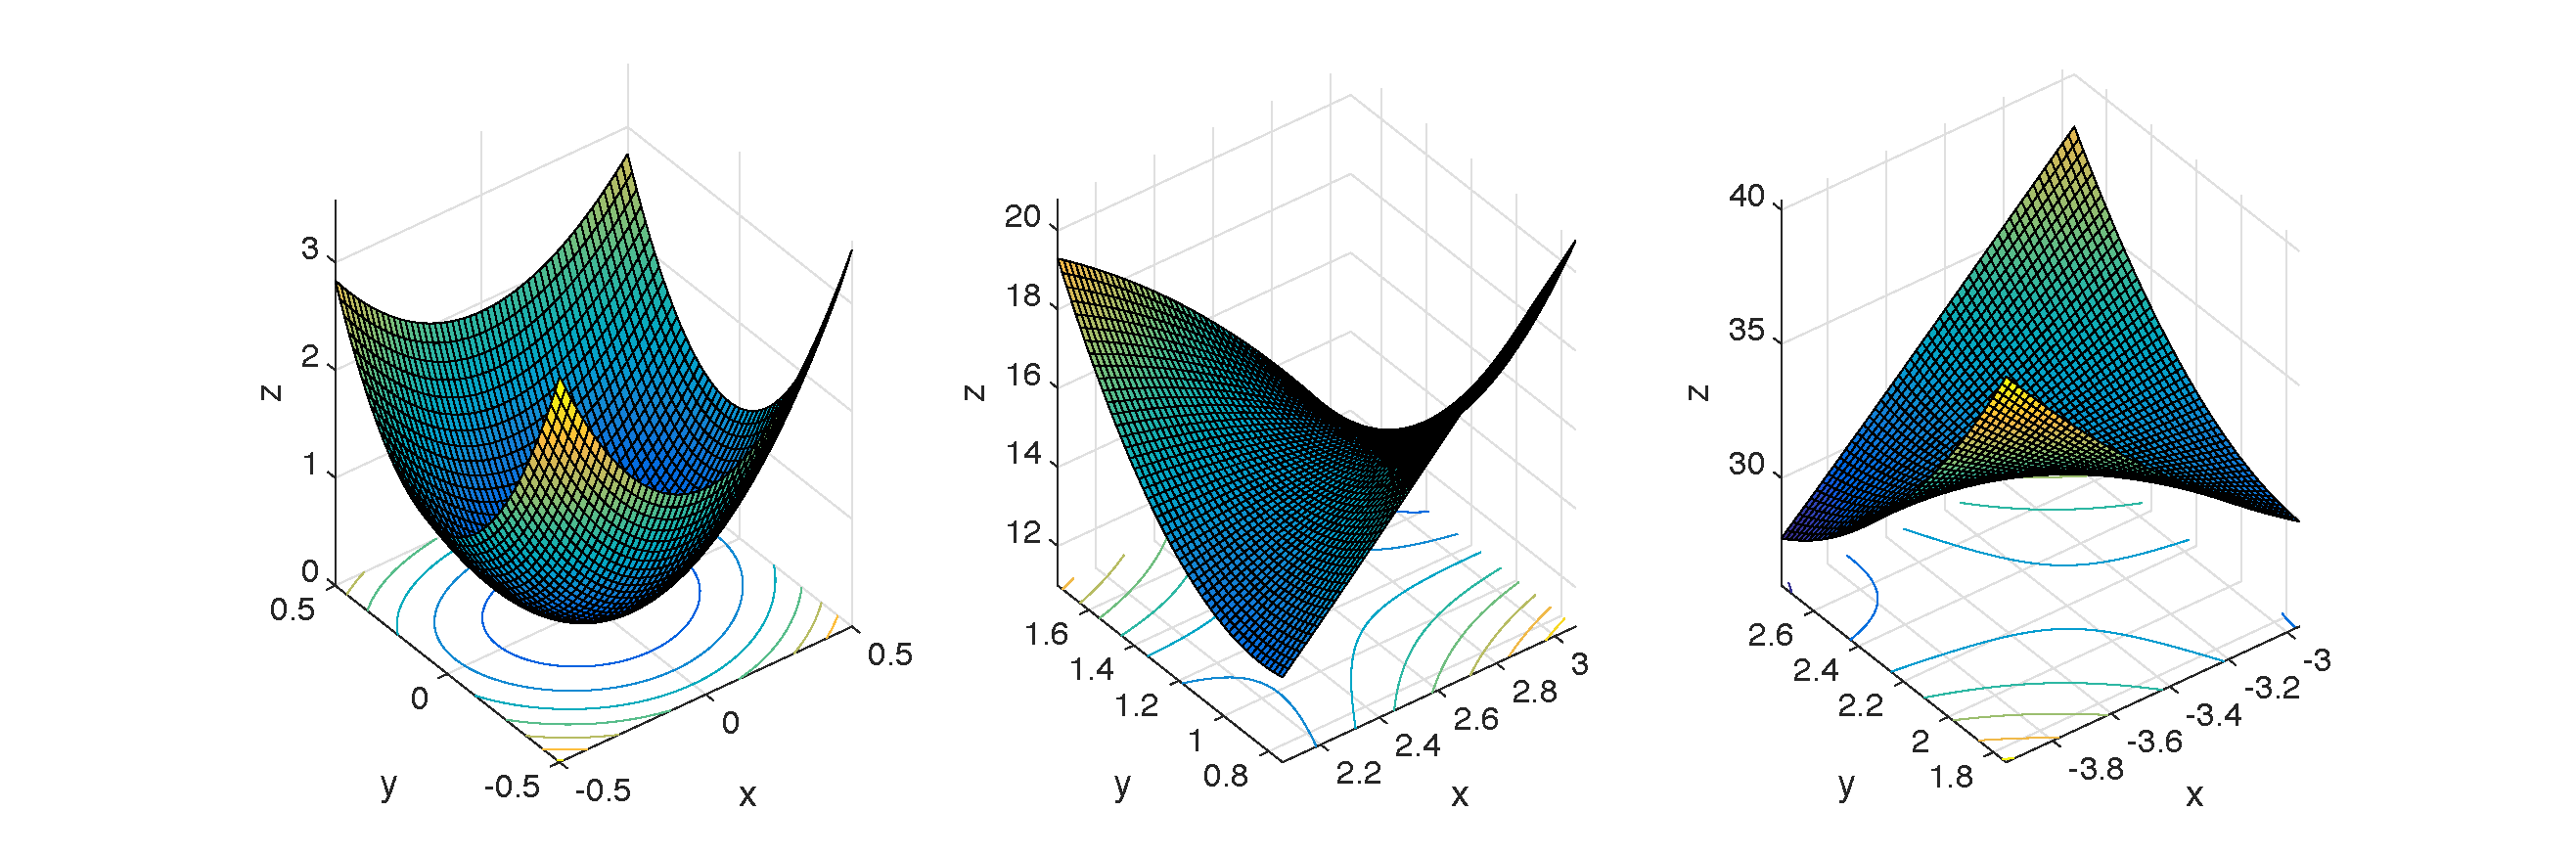
\includegraphics[width = 0.5\textwidth]{Local_min_saddle.pdf}%
%\includegraphics[scale = 1]{eas_boar_1.pdf}%
\caption{Left: Local behaviour near to $(0,0)$ - a "minimum''; Middle: Local behaviour near to $(2.57, 1.24)$ - a "saddle''; Right: Local behaviour near to $(-3.46, 2.24)$ - a "saddle''.}
%\label{PP_sim1}%
\end{figure}


\newpage
\section{The key take home message}

A point $(a,b)$ is a critical point of a function $f(x,y)$ when
$$
\nabla f_{(a,b)} = (0,0)
$$
At such critical points:
\vspace{.5cm}

\framebox(330,60){$ f(x,y) \approx f(a,b) + \frac{1}{2} \left( \begin{array}{c} x-a\\y-b \end{array} \right)^T \left[ \begin{array}{cc}
\frac{\partial ^2 f}{\partial x ^2} & \frac{\partial ^2 f}{\partial x \partial y}\\\frac{\partial ^2 f}{\partial x \partial y} & \frac{\partial ^2 f}{\partial y ^2} \end{array} \right]_{(a,b)} \left( \begin{array}{c} x-a\\y-b \end{array} \right) $}

The behaviour of $f(x,y)$ near to a critical point is governed by the eigenvalues of the Hessian
$$
H = \left[ \begin{array}{cc}
\frac{\partial ^2 f}{\partial x ^2} & \frac{\partial ^2 f}{\partial x \partial y}\\\frac{\partial ^2 f}{\partial x \partial y} & \frac{\partial ^2 f}{\partial y ^2} \end{array} \right]_{(a,b)}  
$$
$H$ is symmetric and is ``diagonalised'' by a rotation of coordinates.


\textbf{Characterising Critical Points}

Let $(a, b)$ be a critical point so that $\nabla f_{(a,b)} = (0,0)$.
\begin{itemize}
\item
If the Hessian $H$ has \textcolor{red}{POSITIVE} eigenvalues, then
\\

$(a, b)$ is a  \textcolor{red}{LOCAL MINIMUM};
\item
If the Hessian $H$ has \textcolor{red}{NEGATIVE} eigenvalues, then
\\

$(a, b)$ is a  \textcolor{red}{LOCAL MAXIUM};
\item
If the Hessian $H$ has eigenvalues of \textcolor{red}{MIXED SIGN} , then
\\ 

$(a, b)$ is a  \textcolor{red}{LOCAL SADDLE};
\end{itemize}



\noindent
\textbf{Example.} Find and characterise the critical points of
$$
f(x,y) = \frac{1}{2} x^2 - \frac{1}{3} x^3 + y^2 - x^2 y\,.
$$
\textbf{Step 1.} Find partial derivatives:
$$
f_x = x - x^2 - 2 x y\qquad f_y = 2y - x^2
$$
\textbf{Step 2.} Set partial derivatives to zero for critical points:
$$
f_x = x - x^2 - 2 x y = 0 \qquad f_y = 2y - x^2 = 0
$$
\textbf{Step 3.} Then
$$
x - x^2 - 2 x y = x (1 - x - 2y) = 0 \quad \mbox{and} \quad x^2 = 2y
$$
Solving for $x$ and $y$: $x = 0 \implies y = 0$ or
$$
1 - x - 2y = 0 \implies (1- 2y)^2 = 2 y \implies 4y^2 - 6y + 1 = 0
$$
Giving critical points
{\small
$$
P_1 = (0,0), \quad P_2 = (-\frac{1+\sqrt{5}}{2},\frac{1}{4}\left( 3+\sqrt{5}\right)), \quad P_3 = (-\frac{1-\sqrt{5}}{2}, \frac{1}{4}\left( 3-\sqrt{5}\right))
$$
}


\noindent
\textbf{Step 4.} Compute the Hessian:
$$
H = \left[ \begin{array}{cc}
\frac{\partial ^2 f}{\partial x ^2} & \frac{\partial ^2 f}{\partial x \partial y}\\\frac{\partial ^2 f}{\partial x \partial y} & \frac{\partial ^2 f}{\partial y ^2} \end{array} \right]
= 
\left[ \begin{array}{cc} 1 - 2x -2y & -2x \\ -2x & 2 \end{array} \right]
$$
{\small
\textcolor{red}{
$$
\mbox{At } P_1 = \left[ \begin{array}{cc} 1 & 0 \\ 0 & 2 \end{array} \right]\,.
\mbox{ At } P_2 = \left[ \begin{array}{cc} 1.62 & 3.23 \\ 3.23 & 2\end{array} \right]\,.
\mbox{ At } P_3 = \left[ \begin{array}{cc} -0.62 & -1.23 \\ -1.24 & 2 \end{array} \right]\,.
$$
}
}
\textbf{Step 5.} Eigenvalues of Hessian at
\begin{itemize}
\item
\textcolor{red}{$P_1$ are $1, 2 \implies \mbox{ local minimum}$}
\item
$P_2$ are $-1.43, 5.10 \implies \mbox{ local saddle}$
\item
\textcolor{red}{$P_3$ are $-1.11, 2.50 \implies \mbox{ local saddle}$}
\end{itemize}


%$$
%f(x,y) = \frac{1}{2} x^2 - \frac{1}{3} x^3 + y^2 - x^2 y
%$$
\begin{figure}[!ht]
\vspace{-2.5cm}
\centering
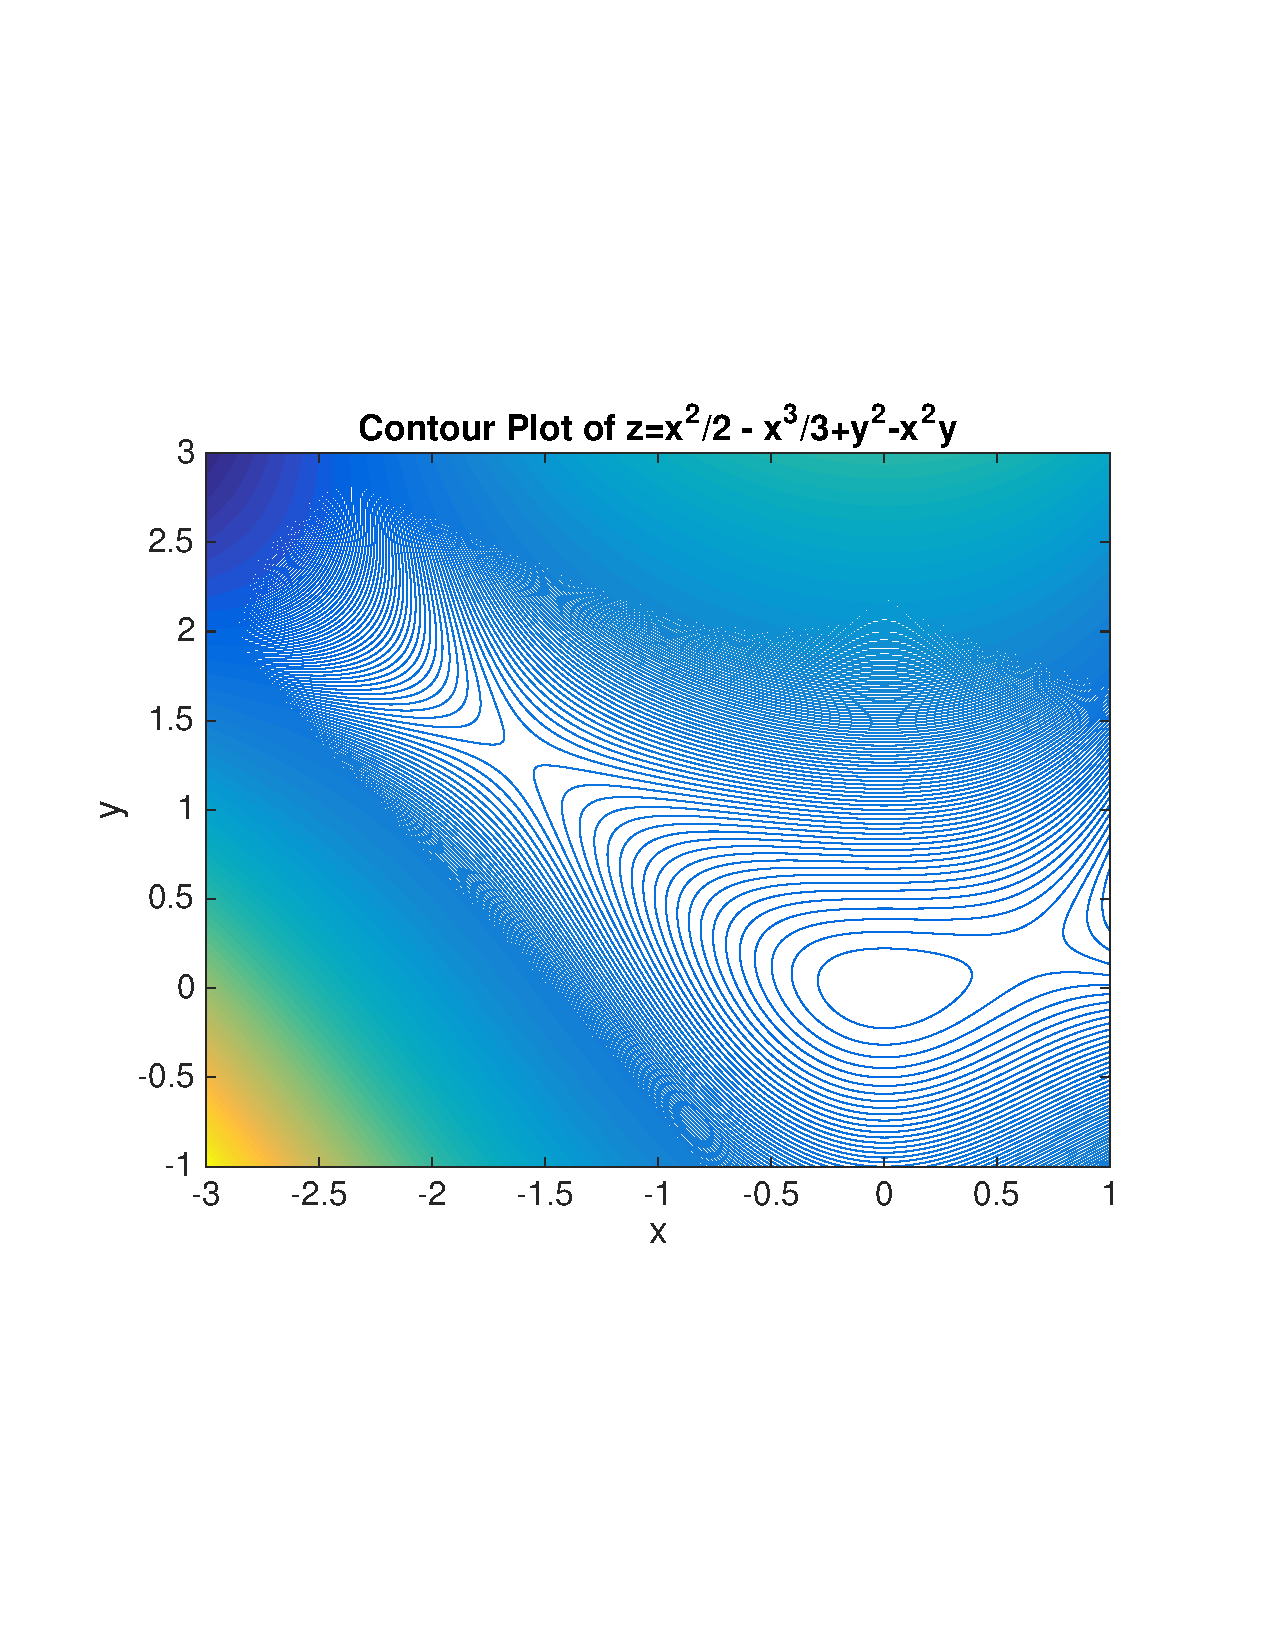
\includegraphics[width = 0.5\textwidth]{TaylorP22.pdf}%
%\includegraphics[scale = 1]{eas_boar_1.pdf}%
\vspace{-3cm}
\caption{Local behaviour near to $(0,0)$ - a "minimum''; 
Local behaviour near to $P_2$ - a ``saddle''; Local behaviour near to $P_3$ - a "saddle''.}
%\label{PP_sim1}%
\end{figure}


\section{Summary}

\begin{itemize}
\item
We can use partial differentiation to characterise the local behaviour of multivariable functions
\item
As with calculus for functions of one variable, we use derivatives to find critical points
\item
Critical points occur where $f_x$ and $f_y$ are simultaneously equal to zero
\item
As with calculus for functions of one variable, we use second order derivatives to check for the type of critical point
\item
We compute the Hessian $H$ at a critical point:
$$
H = \left[ \begin{array}{cc}
\frac{\partial ^2 f}{\partial x ^2} & \frac{\partial ^2 f}{\partial x \partial y}\\\frac{\partial ^2 f}{\partial x \partial y} & \frac{\partial ^2 f}{\partial y ^2} \end{array} \right]
$$
\begin{itemize}
\item
Critical point is a local minimum if $H$ has positive eigenvalues
\item
Critical point is a local maximum if $H$ has negative eigenvalues
\item
Critical point is a saddle if the eigenvalues of $H$ have mixed sign.
\end{itemize}
\end{itemize}

\bigskip

\noindent{\bf Local Maxima and minima of functions of two variables.}

A function of two variables has a local maximum at $(a,b)$ if
$f(x,y)\le f(a,b)$ when $(x,y)$ is near $(a,b)$. A function of two
variables has a local minimum at $(a,b)$ if $f(x,y)\ge f(a,b)$
when $(x,y)$ is near $(a,b)$.

If $f$ has a local maximum or minimum at $(a,b)$ and first-order
partial derivatives of $f$ exist there, then
$$
\frac{\partial f}{\partial x}=0, \;\;  \frac{\partial f}{\partial
y}=0,
$$
at the Point $(a,b)$,
which is called the critical point of the function $f=f(x,y)$.


To find the critical point $(a,b)$, 
we have to solve the two simultaneous
(often nonlinear) equations  ${{\frac{\partial f}{\partial
x}}}=0$, and ${{\frac{\partial f}{\partial y}}}=0$. Often
there are several critical points, not just one. In general,
solving these can be quite difficult.

\bigskip

\noindent{\bf The Second Derivative Test}. These critical points need to be {\it classified} into local
minima, local maxima or saddle points. We need the Second
Derivative Test.  
For some $c$ between $0$ and $1$, we have 
$$
F(1)=F(0)+F'(0)(1-0)+\frac{1}{2} (1-0)^2 F''(c)
$$
without having a remainder.
The two variable Taylor series can be cast in the form
$$
f(x,y)=f(a,b)+ \left( h \frac{\partial f}{\partial x} + k
\frac{\partial f}{\partial y} \right)_{a,b} + \frac{1}{2!} \left( h^2
\frac{\partial^2 f}{\partial x^2} + 2hk \frac{\partial^2
f}{\partial x \partial y} + k^2 \frac{\partial^2 f}{\partial
y^2}\right)_{(a+ch,b+ck)},
$$
where $h=x-a$ and $k=y-b$.
Since
$$
f_x(a,b)=0, \;\; f_y(a,b)=0
$$
$$
f(x,y)-f(a,b)=\frac{1}{2} \left(h^2f_{xx}+2hk
f_{xy}+k^2f_{yy}\right)_{(a+ch,b+ck)}
$$
An extremum of $f$ at the point $(a,b)$ is determined by  the sign of
$$
Q(c)= \left(h^2f_{xx}+2hk f_{xy}+k^2f_{yy}\right)_{(a+ch,b+ck)}
$$
for sufficiently small values of $h$ and $k$. 
{\it If $Q(0) \ne 0$, the sign of $Q(c)$ will be the same as the sign of $Q(0)$
for sufficiently small values of $h$ and $k$. }


Multiply both sides by $f_{xx}$ and rearrange the right-hand side to get
$$
f_{xx} Q(0) =h^2(f_{xx})^2 +2hk f_{xx} f_{xy}+k^2 f_{xx}f_{yy}=
\left(hf_{xx}+kf_{xy})^2 + k^2(f_{xx} f_{yy}- f_{xy}^2 \right)_{(a,b)}.
$$
If the critical point is at $(a,b)$, we must find the numerical
values of
$$
A= { {\frac{\partial^2 f}{\partial x^2}}}, \;  B= {
{\frac{\partial^2 f}{\partial x
\partial y}}}, \;  C= { {\frac{\partial^2 f}{\partial
y^2}}}, \;\; at \;\; x=a, y=b.
$$
Then we need to calculate
$$
\Delta = AC-B^2=\left(f_{xx} f_{yy}- f_{xy}^2 \right)_{(a,b)}.
$$
If $A>0$, and $\Delta>0$ at $(a,b)$, it is a local minimum. \\
If $A<0$, and $\Delta>0$  at $(a,b)$,  it is  a local maximum. \\
If $\Delta<0$, its a saddle point (not a local maximum or minimum).\\
If $\Delta=0$, the test is inclusive and another test is needed. This is because
$Q(0)=0$ prevents us from drawing conclusions about the sign of $Q(c)$.

If there is exact equality in any of these criteria,
we need to start looking at the third order partial derivatives to
study the local behaviour near the critical point. This can be
done, but the algebra gets complicated!

\bigskip

\noindent{\bf Example}. Find the local maximum and minimum values
and saddle points of
$$
f(x,y)=x^4+y^4-4xy+1.
$$
We first locate the critical points
$$
f_x=4x^3-4y, \;\; f_y=4y^3-4x
$$
We have
$$
x^3-y=0, \;\;  y^3-x=0 
$$
$$
 \to \;\;
x^9-x=x(x^8-1)=x(x^4-1)(x^4+1)=x(x^2-1)(x^2+1)(x^4+1)=0
$$
which has the real roots $x=0,1,-1$. The three critical points are
$$
x=0,y=0; \; x=1, y=1; \;\; x=-1, y=-1
$$
use the second Derivative Test,
$$
\Delta(x,y) = AC-B^2=f_{xx} f_{yy}- f_{xy}^2, \;\; f_{xx}=12x^2,
\;\; f_{yy}=12y^2, \;\; f_{xy}=-4.
$$
At the $(0,0)$
$$
\Delta(0,0) =- 4<0, \mbox{ it is a saddle point}
$$
At the $(1,1)$
$$
\Delta(1,1) =12 \times 12 -16=128>0,\;\; f_{xx}(1,1)=12 >0 \mbox{
$f(1,1)=-1$  is a local minimum.}
$$
At the $(-1,-1)$
$$
\Delta(-1,-1) =12 \times 12 -16=128>0,\;\; f_{xx}(1,1)=12 >0
\mbox{ $f(-1,-1)=-1$  is also a local minimum.}
$$

\bigskip

\noindent{\bf Lagrange multipliers.}

This method is used when we are trying to minimise or maximise a
function subject to a constraint. If the constraint is simple
enough, we may be able to eliminate one variable completely. In
this case, we just use the standard method for turning values of
functions of one variable by setting the derivative zero.

However, it may be impractical to eliminate one of the variables.
Then the {\it Lagrange multiplier} method is used.

\begin{enumerate}

\item[(i)] {\it Function of two variables, $f(x,y)$ with one constraint
$g(x,y)=0$}.

Introduce the {\it Lagrange multiplier} $\lambda$ and
$$
F(x,y,\lambda)=f(x,y)+ \lambda g(x,y)
$$
 The Lagrange multiplier equations are
$$ \frac{\partial f}{\partial x} + \lambda \frac{\partial g}{\partial x}=0, $$
$$ \frac{\partial f}{\partial y} + \lambda \frac{\partial g}{\partial y}=0, $$
$$g(x,y)=0.$$
These are three equations for three unknowns, $\lambda$,$x$ and
$y$. You have to find all possible solutions. In general quite
hard, but in examples there is usually a way of simplifying the
Lagrange multiplier equations. There is often more than one
solution. If so, you need to find them all, unfortunately! The
solutions for $x$ and $y$ will be critical points, maxima, minima
or saddle points. Usually, you have to find the maximum or minimum
of $f$, and the easiest way is just to substitute in the critical
values into $f(x,y)$ and find the biggest or the smallest as
required.



\item[(ii)] {\it Function of three variables, $f(x,y,z)$ with one
constraint $g(x,y,z)=0$}. Consider
$$
F(x,y,z,\lambda)=f(x,y,z)+ \lambda g(x,y,z)
$$
The same basic idea works again. Introduce the extra unknown
$\lambda$, the Lagrange multiplier, and solve the four equations
$$ \frac{\partial f}{\partial x} + \lambda \frac{\partial g}{\partial x}=0, $$
$$ \frac{\partial f}{\partial y} + \lambda \frac{\partial g}{\partial y}=0, $$
$$ \frac{\partial f}{\partial z} + \lambda \frac{\partial g}{\partial z}=0, $$
$$g(x,y,z)=0,$$
for the four unknowns, $x$,$y$,$z$ and $\lambda$. The points
$(x,y,z)$ found this way are critical points. Substituting in
gives the value of $f(x,y,z)$ at the critical point. If all the
critical points are found, the global max or min, the largest
overall value of the function can be found.

[ Note: The method can be generalised to find the max/min of
functions of $n$ variables with a constraint. Can also do problems
with more than one constraint. With $m$ constraints you need to
introduce $m$ Lagrange multipliers, see textbooks for details.]

\end{enumerate}

\bigskip

\noindent{\bf Example}. Find the point on the surface
$(x-y)^2-z^2=1$ which is closest to the origin $(0,0,0)$.\\
The distance is
$$
d=\sqrt{x^2+y^2+z^2},
$$
We take
$$
f(x,y,z)=d^2= x^2+y^2+z^2,
$$
with the constraint
$$
(x-y)^2-z^2-1=0.
$$
Let
$$
F(x,y,z, \lambda)= x^2+y^2+z^2 + \lambda \left[ (x-y)^2-z^2-1
\right].
$$
$$
F_x=2x+ 2\lambda(x-y)=0, \;\;  F_y=2y- 2\lambda(x-y)=0,
$$
$$
F_z=2z- 2\lambda z =0,
$$
which gives
$$
z=0, \; or  \; \lambda=1.
$$
Finally, we also have 
$$
(x-y)^2-z^2-1=0.
$$
If $\lambda=1$, then
$$
2x+ 2(x-y)=0, \;\;  2y- 2(x-y)=0, \;\; \to \;\;  2x-y=0, \;\;
-2x+4y=0, \;\; \to \;\; x=0, \; y=0
$$
which yields 
$$
z^2=-1.
$$
Hence, the solution $(0,0)$ and $\lambda=1$ should be excluded. \\

If $z=0$, the sum of 
$$
2x+ 2\lambda(x-y)=0, \;\;  2y- 2\lambda(x-y)=0
$$
gives
$$
2x+ 2y=0, \; \to \;    x=-y,
$$
then, using
$$
(x-y)^2-z^2-1=0,
$$
at $z=0$,
we obtain 
$$
4 x^2=1, \;\; \to \;\; z=0,\;
x=1/2, \; y=-1/2, \;\; \mbox{or} \;\; z=0, \;  x=-1/2, \; y=1/2.
$$
Both solutions yield
$$
d=\sqrt{1/4+1/4+0}=\sqrt{2}/2,
$$

\bigskip

\noindent{\bf Example}. If $x>0, y>0, \;(x+y)=2C$, where $C$ is
constant, show that
$$
\frac{1}{2}(x^n+y^n) \ge \left( \frac{x+y}{2} \right)^n
$$
where $n$ is a positive integer. We shall use $n=5$ as an example.
Let
$$
F(x,y,\lambda)=\frac{1}{2}(x^n+y^n) +\lambda (x+y-2C)
$$
$$
F_x=nx^{n-1}/2+ \lambda=0, \;\; F_y=ny^{n-1}/2+ \lambda=0, \;\;
x+y-2C=0
$$
which has the one critical point, because
$$
n(x^{n-1}-y^{n-1})=0, \;\; x=y, \;\; 2x-2C=0, \;\; x=y=C
$$
use the second Derivative Test,
$$
\Delta(C,C) =\left[ F_{xx} F_{yy}- F_{xy}^2 \right](C,C)=\left[
n(n-1)C^{n-2}/2 \right] \left[ n(n-1)C^{n-2} \right]
-0=\frac{n^2(n-1)^2}{4} C^{2(n-2)}>0,
$$
$$
F_{xx}= \frac{n^2(n-1)}{2} C^{n-2}>0
$$
Hence, $F(C,C)$ is a minimum, i.e.,
$$
\frac{1}{2}(x^n+y^n) \ge \frac{1}{2}(C^n+C^n)=C^n= \left(
\frac{x+y}{2} \right)^n
$$

\part{Multiple Integration}

\section{Double Integrals}
\subsection{Definition and geometric interpretation}

Consider a function $f(x,y)$ defined on a closed rectangle
$$
R = \lbrace a \leq x \leq b, \; c \leq y \leq d \rbrace \,.
$$
The graph $f(x,y)$ is a surface with the equation $z=f(x,y)$.
\begin{figure}[!ht]
\vspace{-.2cm}
\centering
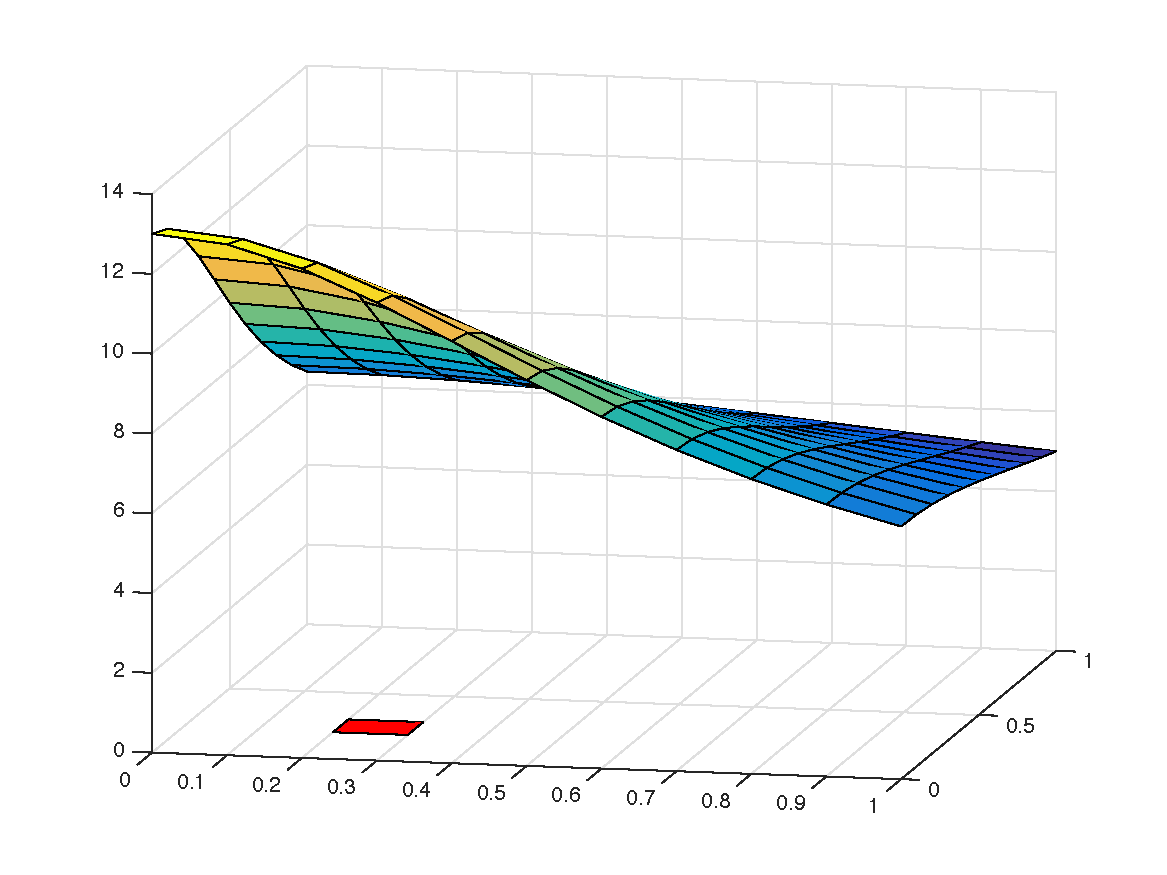
\includegraphics[width = 0.5\textwidth]{MIfig1.pdf}%
%\includegraphics[scale = 1]{eas_boar_1.pdf}%
\label{Surface1}%
\caption{Surface of $z=f(x,y)$ - Looking to compute the volume below the surface, we borrow partition ideas from Riemann Sums}
\end{figure}


Using ideas from Riemann sums we form ``rectangular partitions''
$$
[a, b]: x_0 = a, \ldots , x_m = b; \qquad [c, d]: y_0 = c, \ldots, y_n = d
$$
and then look to approximate the volume by
$$
V \approx \sum_{i=1}^m \sum_{j=1}^n f(x_{ij}^{*},y_{ij}^*)\Delta A_{ij}, \qquad \textcolor{red}{\Delta A_{ij} = (x_i-x_{i-1})(y_j - y_{j-1})}
$$
As with Riemann sums for scalar valued functions: $(x_{ij}^{*},y_{ij}^*)$ is any sample
point in the (\textcolor{red}{red}) rectangle $\lbrace x_{i-1} \leq x \leq x_i, y_{j-1} \leq y \leq y_j \rbrace$

Then the double integral of $f$ over the rectangle $R = \lbrace a \leq x \leq b, \; c \leq y \leq d \rbrace$ is:
$$
I= \int \int_R \, f(x,y) \, dA = \lim_{m,n \to \infty}
\sum_{i=1}^m \sum_{j=1}^n f(x_{ij}^{*},y_{ij}^*)\Delta A_{ij}
$$
when the limit exists and we take finer partitions in the limit.


In the expression
$$
I= \int \int_R \, f(x,y) \, dA = \lim_{m,n \to \infty}
\sum_{i=1}^m \sum_{j=1}^n f(x_{ij}^{*},y_{ij}^*)\Delta A_{ij}
$$
\begin{itemize}
\item
the sum is called a double Riemann sum;
\item
$R$ is the domain of integration, the region of the $xy$-plane
over which the integral is taken;
\item
$f(x,y)$, a function of two variables, is called the {\it integrand}; 
\item
$dA$ is the ``element of area''.
\item
As with integration of functions of one variable, we use the Riemann sum as a formal definition. 
\item
To compute double integrals, if possible we seek to turn them in to a sequence of ``usual'' single integrals.
\end{itemize}

\subsection{Computing double integrals with rectangular domains}

\begin{figure}[!ht]
\vspace{-.2cm}
\centering
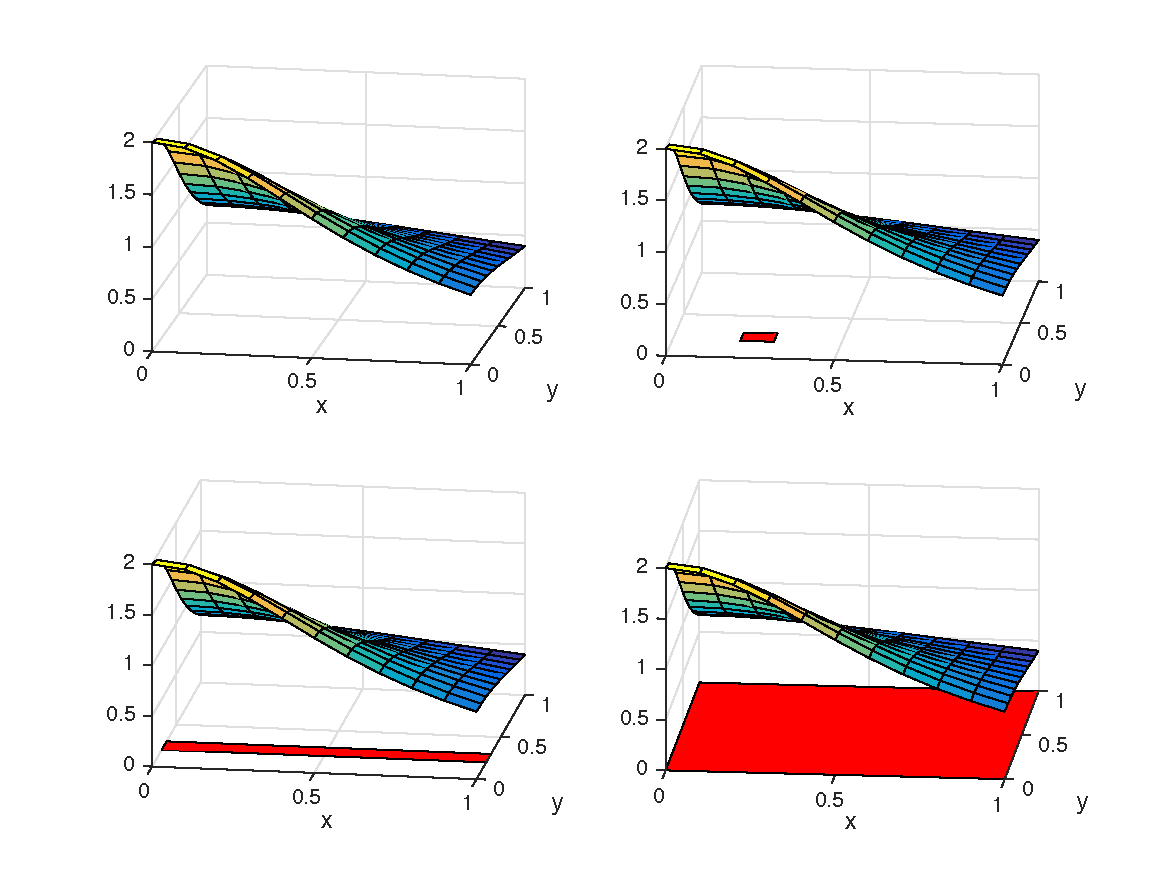
\includegraphics[width = 0.5\textwidth]{dxdy.pdf}%
%\includegraphics[scale = 1]{eas_boar_1.pdf}%
\label{Surface1}%
\caption{Double integrals with rectangular domains. \textbf{Top right}: Compute volume for a rectangular element.
\textbf{Bottom left}: Sum up rectangular elements across $x$ range $\to$ Compute volume for an elemental strip. \textbf{Bottom right}: Sum up volumes of elemental strips $\to$ Total volume.}
\end{figure}


From the Riemann approximation
$$
V \approx \sum_{i=1}^m \sum_{j=1}^n f(x_{ij}^{*},y_{ij}^*)\Delta A_{ij}, \qquad \Delta A_{ij} = (x_i-x_{i-1})(y_j - y_{j-1})
$$
we can rewrite this as
$$
V \approx \underbrace{\sum_{i=1}^m \underbrace{\left( \sum_{j=1}^n f(x_{i}{},y_{j}) (y_j - y_{j-1}) \right)}_{\to \int_c^d f(x_i,y) dy} (x_i-x_{i-1})}_{\to \int_a^b 
\left( \int_c^d f(x,y) dy \right) dx}
$$
where we have chosen $(x_{ij}^{*},y_{ij}^*) = (x_i,y_j)$ in the rectangle $\lbrace x_{i-1} \leq x \leq x_i, y_{j-1} \leq y \leq y_j \rbrace$


Hence for rectangular domains we can express and compute the double integral as two single integrals:
$$
\begin{array}{lll}
\int \int_R \, f(x,y) \, dA & = & \int_a^b \overbrace{\left( \int_c^d f(x,y) dy \right) }^{\textcolor{red}{\mbox{function of } { x} \mbox{  only}}}\textcolor{red}{dx}\\
\\
&& \mbox{integrate first w.r.t. } y, \textcolor{red}{\mbox{  then w.r.t. } x }
\end{array}
$$
OR
$$
\begin{array}{lll}
\int \int_R \, f(x,y) \, dA & = & \int_c^d \overbrace{\left( \int_a^b f(x,y) dx \right)}^{\textcolor{blue}{\mbox{function of } { y}  \mbox{  only}}}\textcolor{blue}{dy}\\
\\
&& \mbox{integrate first w.r.t. } x, \textcolor{blue}{\mbox{  then w.r.t. } y}
\end{array}
$$

%
%\textbf{Geometrical interpretation}: let $z=f(x,y)$ be the height
%of $f(x,y)$ above the $xy$-plane. The domain $R$ is a region of
%the $xy$-plane and the integral $I$ is the volume
%of the region above the $xy$-plane, below the surface $z=f(x,y)$
%and inside the curved surface above the boundary of $D$.
%
%\bigskip
%
%\noindent Note that if $f(x,y)=c$, where $c$ is a constant, then
%the volume is just $c$ times the surface area of $D$, so
%$$
%I = \int \int_D \, c \, dA = c \times \ Area \ of \ D.
%$$
%In
%particular, if $c=1$, then
%$$
%\int \int_D  \, dA = \ Area \ of \ D.
%$$
%
%
%\bigskip
%\noindent  {\bf Rectangular domains}
%
%If the domain $D$ is rectangular, i.e. $x_1 < x < x_2$, $y_1 < y <
%y_2$, then the element of area $dA$ is $dx dy$. We then write
%$$  I = \int \int_D \, f(x,y) \, dx \, dy. $$
%Now fix $y$. The volume above the horizontal strip $(y,y+dy)$ is
%then the area under the curve $f(x,y)$ from $x_1$ to $x_2$ with
%$y$ fixed, times the width $dy$. So volume above the horizontal
%strip $(y,y+dy)$ is
%$$ dy \int_{x_1}^{x_2} f(x,y) \, dx. $$
%Now we have to add up all these little volumes by integrating over
%$y$, so
%$$
%I= \int_{y_1}^{y_2} \Bigl\lbrace \int_{x_1}^{x_2} f(x,y) \, dx \Bigr\rbrace \, dy.
%$$
% So the procedure is to evaluate the inner integral first, keeping
%$y$ constant. The result is then a function of $y$ only, and we
%integrate this function of $y$ to get the desired double integral.
%
%\bigskip
%Notation: $$ \int_{y_1}^{y_2} \Bigl\lbrace
%\int_{x_1}^{x_2} f(x,y) \, dx \Bigr\rbrace \, dy =
%\int_{y_1}^{y_2} \int_{x_1}^{x_2} f(x,y) \, dx \, dy, $$ so we can
%omit the brackets, and we do the inner integral first, i.e. since
%the $dx$ comes before the $dy$ we do the $x$ integral first. The
%limits on the inner integral sign then are the limits for $x$, the
%limits on the outer integral sign being the limits for $y$. It is
%important to remember this, as if the limits are just numbers it
%is not obvious which limits belong to which variable.
%
%\bigskip
%\noindent
% Geometrically, evaluating the $y$ integral
%first means dividing the domain $D$ into vertical strips rather
%than horizontal strips. We are then considering the volume above
%the vertical strip $(x,x+dx)$, which is
%$$ dx \int_{y_1}^{y_2} f(x,y) dy$$
%so adding up all these little volumes gives
%$$
%I= \int_{x_1}^{x_2} \left[ \int_{y_1}^{y_2} f(x,y) \, dy \right]
%\, dx= \int_{y_1}^{y_2} \left[ \int_{x_1}^{x_2} f(x,y) \, dx
%\right]  \, dy.
%$$
%Actually, for rectangular domains we can evaluate the integrals in
%any order and the results are the same.


\textbf{Example}: Find
$$ 
I=\textcolor{red}{\int_{2}^{3}}  \int_{0}^{1}  x \sin \pi y \, dy  \, \textcolor{red}{dx}
$$
So here we mean the \textcolor{red}{outer} $x$ limits are from $2$ to $3$, whilst the \textcolor{blue}{inner} $y$ limits are from $0$ to $1$.

We are integrating over the rectangle
$$
\lbrace 2 \leq x \leq 3, 0  \leq y \leq 1 \rbrace
$$
Thus
$$ 
\begin{array}{lll}
I & = & \textcolor{red}{\int_{2}^{3}} x \left( \int_{0}^{1} \sin \pi y \, dy  \right) \, \textcolor{red}{dx}\\
\\
& = & \textcolor{red}{\int_{2}^{3}} x \left[ - \frac{1}{\pi} \cos \pi y \right]_0^1 \textcolor{red}{dx} \\
\\
& = & \int_{2}^{3} x \frac{2}{\pi} dx \\
\\
& = & \left[ \frac{1}{\pi} x^2 \right]_2^3 = \frac{1}{\pi} \left( 3^2 - 2^2 \right) = \frac{5}{\pi} 
\end{array}
$$


\textbf{Example}: Find
$$ 
I= \int_{0}^{3} \left[  \int_{1}^{2} x^2  y \; dy \right] \; dx 
$$
First, regarding $x$ as a constant, integrating w.r.t. $y$ gives:
{\small
$$
I= \int_{0}^{3} \left[  x^2 (y^2/2)\right]_1^2 \; dx=\int_{0}^{3}
\left[  x^2 (2^2/2)- x^2 (1^2/2) \right]_1^2 \; dx= \int_{0}^{3}
\left[ (3/2) x^2 \right] \; dx
$$
$$
I=  \int_{0}^{3} \left[ (3/2) x^2 \right] \; dx= (3/2)\left[ (1/3)
x^3 \right]_0^3= (3/2)(1/3) 3^3=27/2
$$
}
We can also integrate with respect to $x$ first (regarding $y$ as a
constant)
$$
I= \int_{1}^{2} \left[  \int_{0}^{3} x^2  y \; dx \right] \; dy=
\int_{1}^{2} \left[  (x^3/3) y\right]_0^3 \; dy
$$
$$
=\int_{1}^{2}
\left[ (3^3/3)y \right] \; dy= \left[ (3^3/3) (y^2/2) \right]_1^2
\; = 3^2(2^2-1^2)/2=27/2
$$


\section*{Summary}

\begin{itemize}
\item
To define multiple integrals we first start with \textcolor{red}{rectangular} domains
\item
We partition the rectangle into small rectangles using a regular grid
\item
We approximate the double integral as a volume made from summing up blocks
$$
V \approx \sum_{i=1}^m \sum_{j=1}^n f(x_{ij}^{*},y_{ij}^*)\Delta A_{ij}, \qquad \Delta A_{ij} = (x_i-x_{i-1})(y_j - y_{j-1})
$$
\item
We define the double integral as a limit of sum of blocks as we make the partition (grid) finer and finer
\item
To compute double integrals over rectangular domains we integrate first w.r.t. $y$ (or $x$) and then w.r.t. $x$ (or $y$):
$$
\begin{array}{lll}
\int \int_R \, f(x,y) \, dA & = & \int_a^b \overbrace{\left( \int_c^d f(x,y) dy \right) }^{\textcolor{red}{\mbox{function of } { x} \mbox{  only}}}\textcolor{red}{dx}\\
\\
&& \mbox{integrate first w.r.t. } y, \textcolor{red}{\mbox{  then w.r.t. } x }
\end{array}
$$
\end{itemize}


\subsection{Non Rectangular Domains}

We must (i) identify the domain $R$ in the
$xy$-plane, especially the boundary curves and (ii) decide the order of integration --- $x$ first or $y$ first.
\begin{figure}[!ht]
\vspace{0.25cm}
\centering
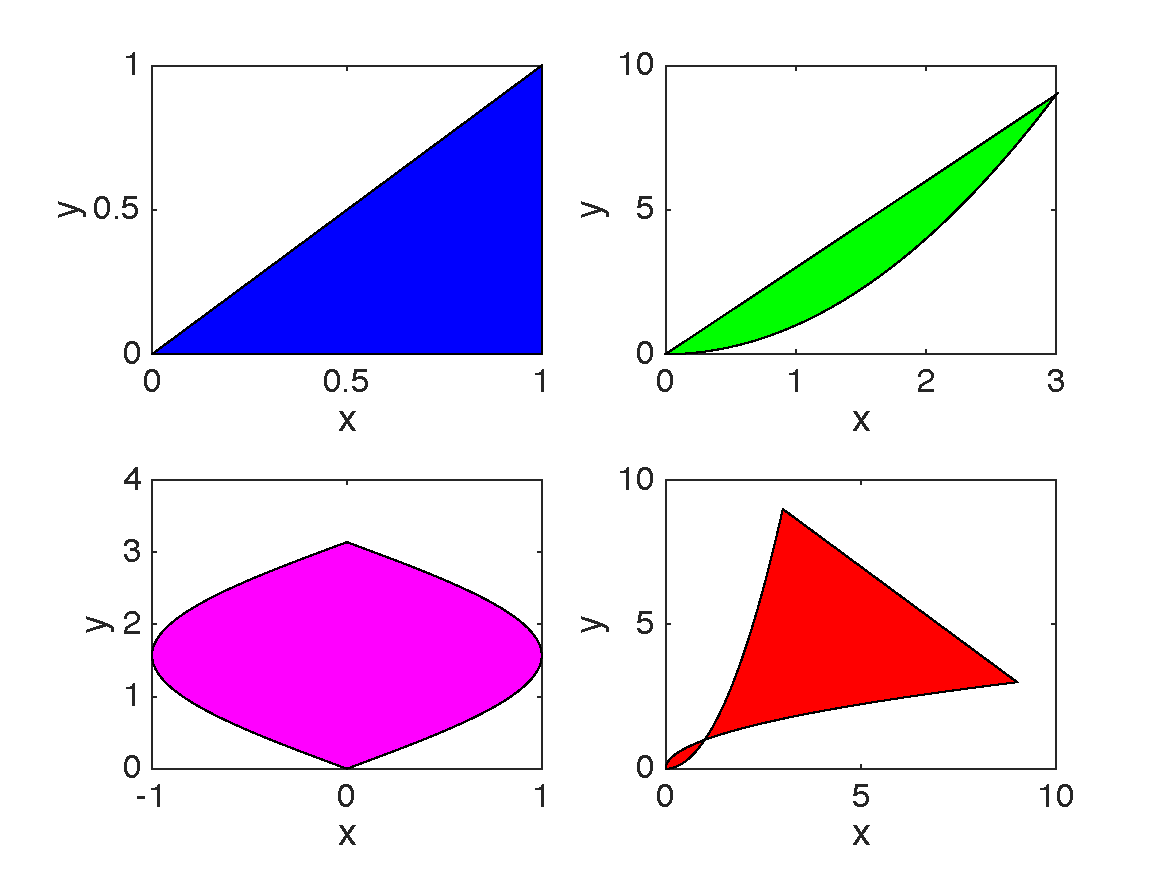
\includegraphics[width = 0.5\textwidth]{Non_rect_doms.pdf}%
%\includegraphics[scale = 1]{eas_boar_1.pdf}%
\vspace{-.3cm}
\caption{\textcolor{blue}{Top Left}: Triangular domain with vertices $(0,0), (1,0), (1,1)$. 
\textcolor{green}{Top right}: Region between the $y = x^2$ and $y=3x$. 
\textcolor{magenta}{Bottom left}: Region between $x = sin(y)$ and $x=-sin(y)$, $0 \leq y \leq \pi$.
\textcolor{red}{Bottom right}: Region between $y=x^2$, $y = \sqrt{x}$ and $x+y = 12$.}
\label{non_rect}%
\end{figure}
\vspace{.25cm}


\textbf{Type I}:  A plane region $R$ lies between the graphs of two
continuous functions of $x$ (\textcolor{green}{green figure above})
$$ 
a \le x \le b,\;  y_1(x) \le y \le y_2(x) \mbox{  with  } y_1(a) = y_2 (a), y_1(b) = y_2(b) 
$$
where we assume that $y_2 (x) \geq y_1 (x)$ for all $x \in [a, b]$.

In this case we fix $x$ between $a$ and $b$ and integrate first w.r.t. $y$
from $y = y_1 (x)$ to $y = y_2 (x)$, and then w.r.t. $x$ from $a$ to $b$.

In this case, the double integral is
$$ 
I= \int_a^b \, \int_{y_1(x)}^{y_2(x)} f(x,y) \, dy \, dx. 
$$
Note we can easily modify this to regions sandwiched between two curves
$$
y = y_1 (x) \quad \mbox{and} \quad y_2 (x)
$$
without the assumption $y_2 (x) \geq y_1 (x)$ by piecing the region together.

%
%\bigskip
%\noindent{\bf Non-rectangular domains}
%
%The first thing is to clearly identify the domain $D$ in the
%$xy$-plane, and in particular the curves denoting the boundaries
%of the domain. We then decide whether to do the $x$ integral first
%(making it the inner integral) or the $y$ integral first.
%
%\bigskip
%
%\noindent
%{\bf Type I} A plane region $D$ lies between the graphes of two
%continuous functions of $x$\\
%$$ a \le x \le b,\;  y_1(x) \le y \le y_2(x). $$
%We choose to do the $y$ integral first by holding $x$ fixed, corresponding to Figures
%below. We next identify the extreme values of $x$ in the domain
%$D$, $x=a$ and $x=b$ in Figures (three different cases). These are
%the limits on the outer $x$ integral. Then we identify the
%boundaries $y=y_1(x)$ and $y=y_2(x)$ of the domain $D$.
%
%\vskip 5cm
%
%
%The double integral is then
%$$ I= \int_a^b \, \int_{y_2(x)}^{y_1(x)} f(x,y) \, dy \, dx. $$
%This means we first integrate $f(x,y)$ with respect to $y$ holding
%$x$ fixed. We evaluate the limits by setting $y=y_2(x)$ and
%$y=y_1(x)$, so that after completing the first integration we are
%left with a function of $x$ only. Then we do the second outer
%integral with respect to $x$, using $a$ and $b$ as the limits.


\textbf{Example} Find
$$  
I = \int \int_R xy \, dy \, dx 
$$
where $R$ is the region in the positive quadrant bounded by 
$$
y=0, x=0 \mbox{  and   } y=1-x^2\,.
$$
First sketch the region $R$.

\vskip 5cm


Extreme values of $x$ are $x=0$ and $x=1$, so these
are the limits of the outer integral. 

At fixed $x$, vertical strips go from $y=0$ to $y=1-x^2$

So the integral is
%$$
%\begin{array}{lll}
%I & = & \int_0^1  \int_0^{1-x^2} xy \, dy \, dx \\
%\\
%& = & \int_0^1 \Bigl[ xy^2/2 \Bigr]_{y=0}^{y=1-x^2} \, dx \\
%\\
%& = & 
%\int_0^1 \frac{x(1-x^2)^2}{2} \, dx = \Bigl[\frac{x^2}{4} - \frac{x^4}{4}
%+\frac{x^6}{12}\Bigr]_0^1 = \frac{1}{12}.
%\end{array}
%$$

\vskip 5cm

%

\textbf{Type II} A plane region $R$ lies between the
graphs of two continuous functions of $x_1(y)$ and $x_2 (y)$ (\textcolor{magenta}{magenta figure above})
$$ 
c \le y \le d,\;  x_1(y) \le x \le x_2(y). 
$$
\vspace{-.8cm}

\begin{itemize}
\item
In this case, we do the $x$ integral first.
\item
We identify the extreme values $y=c$ and $y=d$. 
\item
These are the limits for the outer $y$ integral. 
\item
We identify the boundaries $x=x_1(x)$ and $x=x_2(x)$ of the domain $R$.
\item
The double integral is then
$$ 
I= \int_c^d \, \int_{x_1(y)}^{x_2(y)} f(x,y) \, dx \, dy\,, 
$$
meaning we: (i) first integrate $f(x,y)$ with respect to $x$ holding
$y$ fixed; (ii) evaluate the limits by setting $x=x_2(y)$ and
$x=x_1(y)$, leaving a function of $y$ only; (iii) integrate w.r.t. $y$, using $c$ and $d$ as the limits.
\end{itemize}

%


\textbf{\bf Example:} Find
$$  
I = \int \int_R xy \, dy \, dx 
$$
where $R$ is the region bounded by the line  $y=x-1$ and the
parabola $y^2=2x+6$.

First sketch the region $R$ (Type II).
\vskip 5cm


 The Type II region is
$$ 
-2 \le y \le 4,\;  y^2/2-3 \le x \le y+1
$$
with intersections between the line $y=x-1$ and the
parabola $y^2=2x+6$ at $(-1,-2)$ and $(5,4).$

Hence, the extreme values for $y$ are $y=-2$ and $y=4$, so these
are the \textcolor{red}{limits} of the outer integral. 

At fixed $y$, horizontal
strips go from $x=y^2/2-3$ to $x=y+1$, so the integral is
$$
\begin{array}{lll}
I & = & \int \int_R xy \, dy \, dx = \int_{-2}^4 \int_{y^2/2-3}^{y+1} xy \, dx \, dy\\
  & = & \int_0^1 \Bigl[ x^2y/2 \Bigr]_{x=y^2/2-3}^{x=y+1} \, dy \\
 & = &  \frac{1}{2} \int_{-2}^4 y \left[(y+1)^2-(y^2/2-3)^2\right] \; dy \\
 & = & \frac{1}{2} \int_{-2}^4 \left[-y^5/4 +4 y^3+2y^2-8y \right] \; dy \\
 & = & \frac{1}{2} \left[-y^6/24 +y^4+2y^3/3-4y^2 \right]_{-2}^{4}=36.
 \end{array}
$$


\textbf{Further Example:} Find
$$
I = \int \int_R x y^{1/2} \, dx \, dy
$$
where $R$ is the region in the positive quadrant bounded by the parabolas 
$$
y=\sqrt{x} \mbox{  and  } y=x^2.
$$
This is a Type I region: We sketch the region: $0 \le x \le 1, x^2 \le y \le \sqrt{x}$.
\vskip 5cm



The integral is
$$
\begin{array}{lll}
I & = & \int_0^1  \int_{x^2}^{\sqrt{x}} xy^{1/2} \, dy \, dx \\
\\
 & = &  \int_0^1 x \Bigl[ 2y^{3/2}/3 \Bigr]_{y=x^2}^{y=\sqrt{x} } \, dx \\
 \\
 & = & \int_0^1 \frac{2}{3} x( x^{3/4}-x^3) \, dx =\frac{2}{3} \Bigl[\frac{4 x^{11/4}}{11} - \frac{x^5}{5} \Bigr]_0^1 \\
 \\
 & = & \frac{2}{3} \Bigl[\frac{4}{11} - \frac{1}{5} \Bigr]  = \frac{6}{55}.
 \end{array}
$$


\textbf{Example:} If $f(x)$ is continuous on $[0,1]$ and
$$
\int_0^1 f(x)\, dx = \alpha,
$$
then find the value of
$$
I = \int_0^1 \int_x^1 f(x) f(y)  \, dy \, dx.
$$
First sketch the region $R$: $ 0 \le x \le 1, x \le y \le 1$.

\vskip 5cm


%

$R$ is triangular. So we first change the order of the integration
$$
\int_0^1 \left[ \int_x^1 f(x) f(y)  \, dy  \right] \, dx = \int_0^1 \left[ \int_0^y f(x) f(y)  \, dx  \right] \, dy.
$$
If we interchange $x$ and $y$, then the second version of the integral can be written:
{\small
$$
I=\int_0^1 \left[ \int_0^x f(y) f(x)  \, dy  \right] \, dx
$$
}
Then adding
$$
\int_0^1 \left[ \int_x^1 f(x) f(y)  \, dy  \right] \, dx \mbox{  and  } \int_0^1 \left[ \int_0^x f(y) f(x)  \, dy  \right] \, dx
$$
we see that
$$
2 I = \int_0^1 \int_0^1 f(x) f(y) dy dx  = \int_0^1 f(x) dx \int_0^1 f(y) dy = \alpha^2
$$
so that 
{\small
$$
I=\frac{\alpha^2}{2}\,.
$$
}


To find the area of a region we simply compute the double integral
$$
\mbox{Area of  } R = \int \int_R \, 1 \, dx dy
$$
that is where the integrand is the constant function $f(x,y) = 1$


\section*{Summary}

\begin{itemize}
\item
To compute integrals over non-rectangular domains we first \textcolor{red}{draw a picture of the domain}
\item
Then we look to see if the domain is sandwiched between curves:
$$
y = y_1 (x) \mbox{ and } y = y_2 (x) \quad \mbox{OR} \quad x = x_1 (y) \mbox{ and } x = x_2 (y)
$$
\item
If the former or \textcolor{blue}{latter}, then the integral is
$$ 
I= \int_a^b \, \int_{y_1(x)}^{y_2(x)} f(x,y) \, dy \, dx \qquad \mbox{OR} \qquad  \textcolor{blue}{I= \int_c^d \, \int_{x_1(y)}^{x_2(y)} f(x,y) \, dx \, dy}
$$
\item
For double integrals over more complicated domains, we look to break the domain up into several portions, each sandwiched between curves ($y=y_1 (x), y=y_2(x)$ or $x = x_1(y), x=y_2 (x)$).
\end{itemize} 



\bigskip

Sometimes, the integrand is not differentiable. For example, the
function $\vert x-y \vert$, the modulus of $x-y$, is not smooth
across the line $x=y$. In this situation, you need to break the
region $D$ into two regions, one on one side of $x=y$, the other
on the other side. Evaluate both integrals, and add the result.

First sketch the region $D$, where $D_1$ and $D-2$ do not overlap.

\vskip 5cm
%
$$
\int \int_D \, f(x,y) \, dA = \int \int_{D_1} \, f(x,y)\, dA +
\int \int_{D_2} \, f(x,y) \; dA .
$$


\bigskip

\noindent{\bf Example:} Evaluate
$$
I = \int \int_D | 3x+4y| \, dx \, dy
$$
where $D$ is the region given by $ x^2+y^2 \le a^2$.

\vskip 5cm


The line $3x+4y=0 $ intercepts with the circle  $ x^2+y^2 \le a^2$
at the two points $A=(4 a/5, -3a/5)$ and $B=(-4 a/5, 3a/5)$. In
polar coordinates, we can divide the region $D$ into the two
regions:
$$
D_1: \theta_0 \le \theta \le  \theta_0+ \pi; \;\; D_2: \theta_0
+\pi \le \theta \le  \theta_0+ 2\pi,
$$
where $\cos \theta_0= 4/5$ and $\sin \theta_0=-3/5$.

In the region $D_1$, we have $ 3x+4y>0$; In the region $D_2$, we
have $ 3x+4y <0$. Then
$$
I = I_1+I_2= \int_{\theta_0}^{\theta_0+\pi} \int_0^a r( 3 \cos
\theta+4r \sin \theta ) r  \, dr \, d \theta + (-1) \int_{\theta_0
+\pi}^{\theta_0+2\pi} \int_0^a r( 3 \cos \theta+4 \sin \theta ) r
\, dr \, d \theta
$$
First, look at the second integral by letting $\theta=\phi + \pi$,
$$
I_2= (-1) \int_{\theta_0 +\pi}^{\theta_0+2\pi} \int_0^a r( 3 \cos
\theta+4 \sin \theta ) r \, dr \, d \theta=(-1) \int_{\theta_0
}^{\theta_0+\pi} \int_0^a  \left[ 3 \cos (\pi +\phi)+4 \sin(\pi
+\phi) \right]  r \, dr \, d \theta
$$
But $\cos (\pi +\phi)=-\cos \phi,\; \sin(\pi +\phi)=-\sin \phi$.
Hence
$$
I_2= \int_{\theta_0 }^{\theta_0+\pi} \int_0^a r \left( 3 \cos
\phi+ 4 \sin \pi \right)  \;  r \, dr \, d \theta =I_1
$$
i.e.,
$$
I = 2I_1= 2\int_{\theta_0}^{\theta_0+\pi}  ( 3 \cos \theta+4 \sin
\theta ) \left[ \int_0^a r^2  \, dr \right] \, d \theta=\frac{2
a^3}{3} \int_{\theta_0}^{\theta_0+\pi}  ( 3 \cos \theta+4 \sin
\theta ) d \theta
$$
$$
I = \frac{2 a^3}{3} \left[ 3 \sin \theta-4 \cos \theta
\right]_{\theta_0}^{\theta_0+\pi}=
$$
$$
I=\frac{2 a^3}{3}\left[ 3 \sin(\pi+ \theta_0)-4 \cos
(\theta_0+\pi) \right]- \frac{2 a^3}{3}\left[ 3 \sin \theta_0-4
\cos \theta_0 \right]=-2 \frac{2 a^3}{3} \left[ 3 \sin \theta_0-4
\cos \theta_0 \right]
$$
$$
=-2 \frac{2 a^3}{3}\left(-3 \frac{3}{5} -4 \frac{4 }{5} \right)=2
\frac{2 a^3}{3} \frac{25}{5}= \frac{20 a^3}{3}.
$$

\bigskip

\section{Polar Coordinates}

\begin{figure}[!ht]
\vspace{-.5cm}
\centering
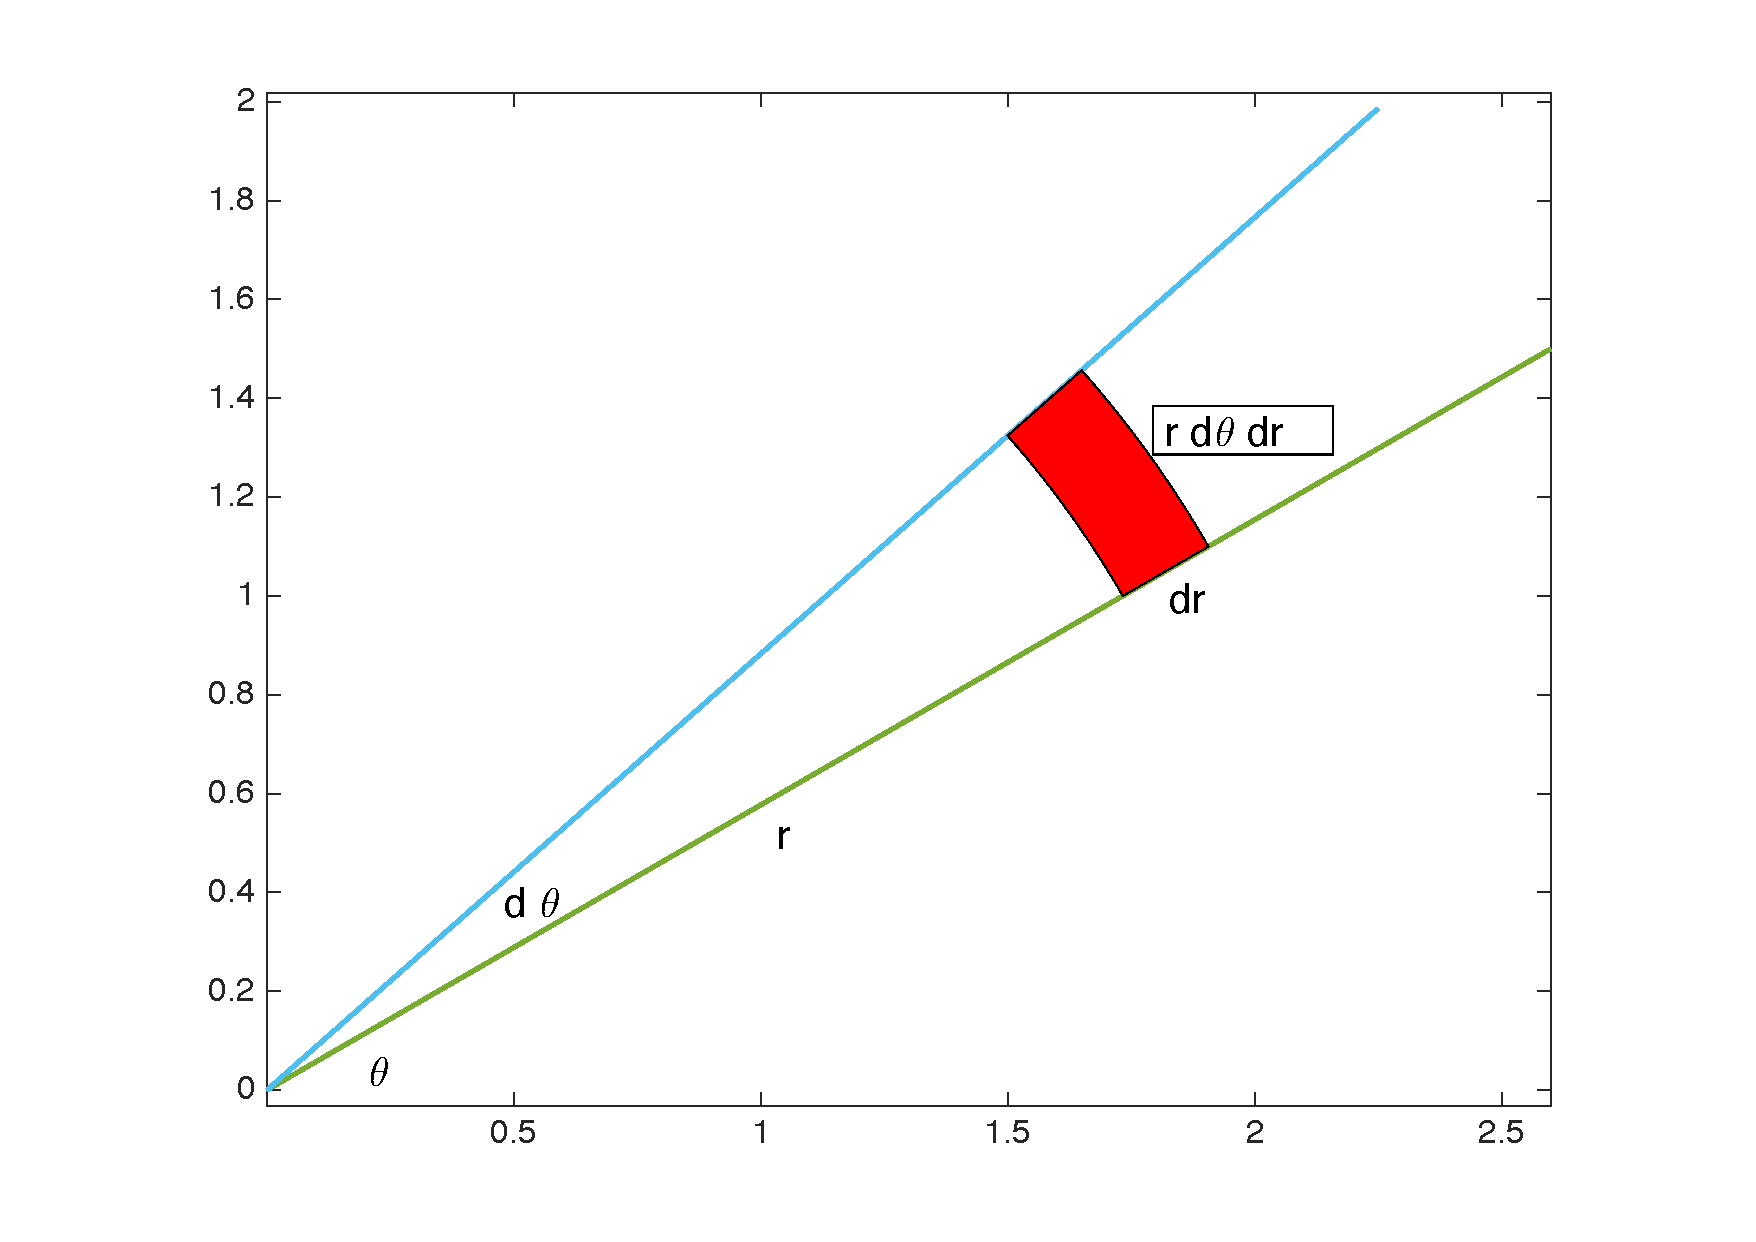
\includegraphics[width = 0.5\textwidth]{polar_stuff.pdf}%
\caption{Polar coordinates. Elemental area (in red) has area $ r d \theta  \times dr$}
\label{polar_element}
\end{figure}

%

In polar coordinates $r, \theta$:
\begin{itemize}
\item
$r$ is the distance from the origin, 
\item
$\theta$ the angle, measured counter-clockwise from the $x$-axis. 
\end{itemize}
Polar coordinates are related to Cartesian coordinates by:
{\small
$$
\begin{array}{lll}
x & = & r \cos \theta, \quad y=r \sin \theta, \\
r & = & \sqrt{x^2+y^2} \quad \theta = \tan^{-1} y/x
\end{array}
$$
}
In polar coordinates the area element is 
$$
\textcolor{red}{dA = r dr d \theta}
$$
This can be seen using a geometrical argument: in Figure \ref{polar_element} the
``rectangular'' element (in red) has area \textcolor{red}{$dr \times r d \theta$}.

If $f$ is continuous on a polar rectangle 
$$
R =  \lbrace 0 \le a
\le r \le b, \; \alpha \le \theta \le \beta\rbrace\,,
$$ 
then
$$
\int \int _R f(x,y) \; d A = \int_{\alpha}^{\beta} \int_a^b f( r
\cos \theta, r \sin \theta) \,\textcolor{red}{r \; dr \;  d \theta}.
$$



\textbf{Example:} Find
$$
I = \int \int_R (x+y) \, dA
$$ where $R$ is the semicircle $\lbrace 0 \leq r \leq 2$, $0 \leq  \theta \leq \pi \rbrace$.
\vspace{2mm}

In polar coordinates, $x+y = r \cos \theta + r \sin \theta$, so
$$
\begin{array}{llll}
I & = & \int_0^{\pi} \int_0^2 r (\cos \theta + \sin \theta) \, \, r \,dr\; d \theta & \\
\\
 & = & \int_0^{\pi}  \left[ r^3/3 \right]_0^3 (\cos \theta + \sin \theta) \, d \theta \quad & r \mbox{ integral first}\\
 \\
 & = & (8/3)  \Bigl[ \sin \theta - \cos \theta \Bigr]_0^{\pi} & \mbox{then the } \theta \mbox{ integral}\\
 \\
  & = & (8/3) [1+1] = \frac{16}{3}. &
  \end{array}
$$


\textbf{Example:}  Find the area enclosed by one petal of the
four-petalled rose given by the polar curve $r=\cos 2 \theta$:
$$
-\pi/4 \le \theta \le \pi/4, \; 0 \le r \le \cos 2 \theta.
$$
\begin{figure}[!ht]
\vspace{-.5cm}
\centering
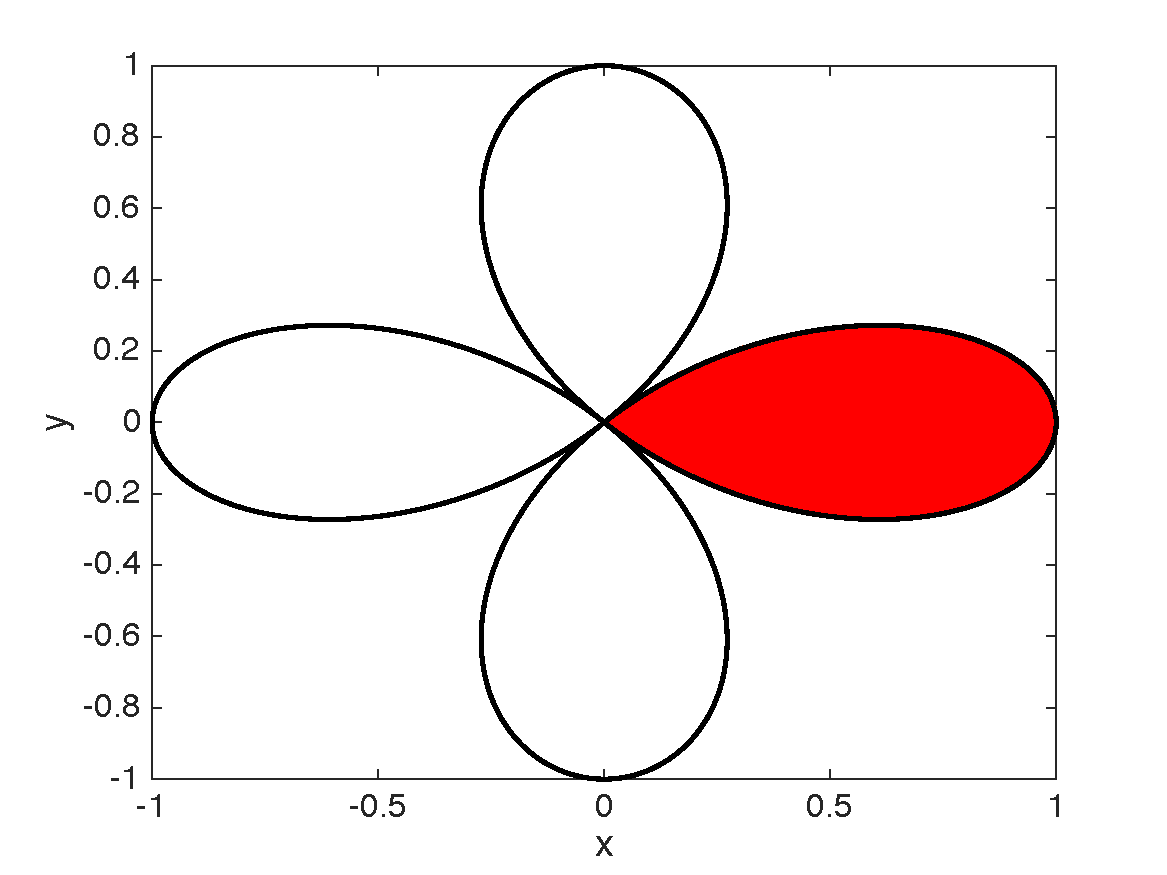
\includegraphics[width = 7cm]{rose.pdf}%
\caption{Region shaded in red is $\lbrace -\pi/4 \le \theta \le \pi/4, \; 0 \le r \le \cos 2 \theta \rbrace$.}
\label{rose}
\end{figure}


The area is
$$
\begin{array}{lll}
\int \int_{\rm petal} & = & \int_{-\pi/4}^{\pi/4} \int_0^{\cos 2
\theta} r dr d \theta \\
\\
 & = & \int_{-\pi/4}^{\pi/4} \left[ r^2/2
\right]_0^{\cos 2 \theta} \; d \theta \\
\\
 & = & \int_{-\pi/4}^{\pi/4}  \frac{1}{2} \cos^2 2\theta \; d \theta\\
 \\
  & = & \int_{-\pi/4}^{\pi/4}  \frac{1}{4} (1+\cos 4 \theta) \; d \theta\\
  \\
   & = & \frac{1}{4} \left[\theta+  \frac{1}{4} \sin 4 \theta \right]_{-\pi/4}^{\pi/4}=
\frac{\pi}{8}
\end{array}
$$


Find
$$
I = \int_{-\infty}^{\infty} e^{-x^2} dx\,.
$$
We use a little trick:
$$
\begin{array}{lll}
I^2 & = & \int_{-\infty}^{\infty} e^{-x^2} dx \int_{-\infty}^{\infty} e^{-y^2} dy\\
\\
& = & \int_{-\infty}^{\infty} \int_{-\infty}^{\infty} e^{-(x^2 + y^2)} dx dy\\
\\
 & = & \int_0^{2\pi} \int_0^\infty e^{-r^2} r dr d \theta\\
 \\
 & = & \int_0^{2\pi} \int_0^\infty \frac{d}{dr} \frac{1}{2} e^{-r^2} dr d \theta\\
 \\
 & = & \frac{1}{2} \int_0^{2\pi} 1 d \theta = \pi
 \end{array}
$$
Hence
$$
\int_{-\infty}^{\infty} e^{-x^2} dx = \sqrt{\pi}
$$


\section{Triple integrals}
\subsection{Cartesian coordinates}

We seek to compute integrals for 3D domains:
$$
I = \int \int \int_V f(x,y,z) \, dV
$$
Now instead of a region $R$ in the plane, the region of
integration is a region $V$ of three-dimensional space.

As in 2D, rectangular boxes are the easiest to deal with.
 
Then the \textcolor{red}{\bf element of volume} is
$$
dV = dx\, dy \, dz
$$ 
and the box is the region 
$$
\lbrace x_1 \leq x \leq x_2, \,\,y_1 \leq y \leq y_2, \,\, z_1 \leq z \leq z_2 \rbrace \,.
$$
So
$$
I = \int_{z_1}^{z_2} \int_{y_1}^{y_2} \int_{x_1}^{x_2} f(x,y,z) \,
dx \, dy \, dz. 
$$ 
As in two dimensions, the integrations can be
done in any order.


If $f(x,y,z)=1$, then the triple integral represents the volume of $V$:
$$
V = \int \int \int_V  dV.
$$


Handling non-rectangular domains in 3D is a tricky (because it is more difficult to 
visualise that the 2D counterpart).
\begin{itemize}
\item
Decide the order of integration
\item
Suppose the $z$ integral is the outermost integral
\item
Find the extreme values of $z$, say $z_1$ and $z_2$ --- these
are the limits of the outermost integral. 
\item
Find the limits on the middle $y$ integral, take $z$ as fixed and find the extreme
values of $y$ as $x$ varies --- it may help to
sketch in the $xy$-plane the boundary of a $z = const.$ slice of
$V$. 
\item
These extreme values of $y$ will be a function of $z$ only --- in general the limits on $y$ will be $y=f(z)$ and $y=g(z)$, some $f$ and $g$.
\item
Then finally the limits on $x$ are determined from the bounding surface
of $V$, which has to be put in the form $x= u(y,z)$,$x=v(y,z)$
where $u$ and $v$ are the lower and upper values of $x$ at fixed
$y$ and $z$.
\end{itemize}



\textbf{Example}: Find the $x, y, z$ limits when $V$ is the sphere
$$
x^2+y^2+z^2 \leq 1.
$$
\vspace{-.5cm}

\begin{itemize}
\item
Extreme values of $z$ are $\pm 1$. 
\item
Now fix $z$ and look for extreme values of $y$. $y= \pm \sqrt{1-z^2-x^2}$. 
\item
The biggest value of $y$ as $x$ varies is at $x=0$ when $y=\sqrt{1-z^2}$. The
smallest value of $y$ is $y=-\sqrt{1-z^2}$. so the limits on $y$
are $\pm \sqrt{1-z^2}$. 
\item
When $z$ and $y$ are fixed, $x=\pm
\sqrt{1-y^2-z^2}$ on the boundary of the sphere, so these are the
limits on $x$. 
\end{itemize}
In this case
{\small
$$
\int \int \int_V f(x,y,z) \, dx \, dy \, dz
= \int_{-1}^{1} \int_{-\sqrt{1-z^2}}^{\sqrt{1-z^2}}
\int_{-\sqrt{1-z^2-y^2}}^{\sqrt{1-z^2-y^2}} f(x,y,z) \, dx \, dy
\, dz.
$$
}


\subsection{Cylindrical and spherical polar coordinates}

\textbf{Cylindrical polar coordinates}. A point $P$ has coordinates $(s,\phi,z)$
where 
\begin{itemize}
\item
$s$ is the distance from the $z$-axis, 
\item
$\phi$ is the usual polar coordinate angle of $P$ from the $xz$-plane, and 
\item
$z$ is the same as the Cartesian $z$
\end{itemize}
Cartesian and cylindrical polar coordinates are linked by:
$$
x=s \cos \phi, \; y=s \sin \phi, \; z=z
$$
{\bf The element of volume} is $dV = s \, ds \, d\phi \, dz.$



\textbf{Example:} Evaluate
$$
 \int \int \int_V s^3 \, dV,
$$
 where $V$ is the cylindrical region 
 $$
 \lbrace 0 \leq s  \leq 2, -1 \leq z \leq 1, 0 \leq \phi \leq 2 \pi \rbrace.
 $$
$$
\begin{array}{lll}
I & = & \int_{-1}^{1} \int_0^{2 \pi} \int_0^2 s^4 \, ds\, d \phi \, dz \\
\\
 & = & \int_{-1}^{1} \int_0^{2 \pi} \Bigl[ \frac{s^5}{5} \Bigr]_0^2 \, d \phi \, dz\\
 \\
  & = & \int_{-1}^{1} \Bigl[ \frac{32}{5} \phi \Bigr]_0^{2 \pi} \, dz\\
  \\
   & = & \int_{-1}^{1} \frac{64\pi}{5} \, dz = \frac{128\pi}{5}.
\end{array}
$$



\textbf{Spherical polar coordinates}. A point $P$ has coordinates $(r, \theta,
\phi)$. 
\begin{itemize}
\item
$\phi$ is the longitude angle, sometimes called the azimuthal angle, measured from the
$xz$-plane
\item
$r$ is the distance from the origin
\item
$\theta$ is the angle from the north pole (the positive $z$-axis). $\theta$ is
sometimes called the co-latitude because it is
$90^{\circ}$-latitude. 
\item
The equator (latitude $0^{\circ}$) has
$\theta = \pi/2$. The South Pole has $\theta = \pi$. 
\end{itemize}
Cartesian and spherical polar coordinates are linked by:
$$
x=r \cos \phi \sin \theta, \;\; y=r \sin \phi \sin \theta, \;\;
z=\cos \theta
$$
{\bf The element of volume} is $dV = dx \, dy \, dz= r^2 \sin \theta \, dr
\, d \theta \, d \phi$.

%


\textbf{Example:}  Evaluate
$$
\int \int \int_V r^3 \,dV,
$$
where $V$ is the hemispherical region 
$$
\lbrace 0 \leq r \leq 2, 0 \leq \theta \leq 
\pi / 2, 0 \leq \phi \leq 2 \pi \rbrace\,.
$$
$$
\begin{array}{lll}
I & = & \int_{0}^{2 \pi} \int_0^{\pi /2} \int_0^2 r^5 \sin \theta \, dr \, d \theta \, d \phi\\
\\
 & = & \int_{0}^{2 \pi} \int_0^{ \pi /2 } \Bigl[ \frac{r^6}{6} \Bigr]_0^2 \, d \theta \, d \phi \\
 \\
 & = & \int_{0}^{2 \pi} \Bigl[ - \frac{32}{3} \cos \theta \Bigr]_0^{ \pi /2} \, d \phi \\
 \\
  & = &  \int_{0}^{2 \pi} \frac{32}{3} \, d\phi = \frac{64\pi}{3}.
\end{array}
$$


\section*{Summary}

\begin{itemize}
\item
Sometimes the domain of integration looks simpler in alternative coordinates
\item
For example a circular domain $x^ 2 + y^2 \leq 4$ is more easily described as a rectangular domain $r \leq 2, \theta \in [0, 2\pi]$.
\item
So we change coordinates, remembering to change $dx\,dy$ in to the relevant elemental area, e.g. in polar coordinates
$$
dx\,dy \mapsto r \,dr \, d\theta
$$
\item
Triple integrals are defined similarly to double integrals
\begin{itemize}
\item
Start with rectangular domains; 
Make small rectangular boxes;
Add up all the boxes and take the limit
\item
In practice, we compute the triple integral as a sequence of three single integrals.
\end{itemize}
\end{itemize}


\newpage

\part{Appendix}

\section{Linear Independence of Functions}

A set of functions $\lbrace f_1, \ldots , f_n \rbrace$, where each $f_i : D \mapsto \mR$ for some common domain $D$
(usually an interval), are \textcolor{red}{linear independent} if
$$
\sum_{j = 1}^n c_j f_j (x) = 0\quad \mbox{for all} \quad x \in D
$$
implies $c_1 = \ldots = c_n = 0$.

We use this concept to make sure that when we solve a differential equation, we are constructing
a general solution.

That is we do not want one function in the solution to be another function in disguise.


\section{Linear Independence of Common Functions}
\subsection{Polynomials}

\textcolor{blue}{The set of polynomial functions $f_i : x \mapsto x^{i-1}$, $i = 1, \ldots, n$, defined on some interval $[0, b], b > 0$, are linearly independent.}

To see this, suppose that
\begin{equation}
\label{poly}
c_1 + c_2 x + \ldots + c_n x^{n-1} = 0 \mbox{   for all   } x \in [0, b]\,.
\end{equation}
\begin{itemize}
\item
Putting $x = 0$ in (\ref{poly}) gives $c_1 = 0$. 
\item
Differentiating (\ref{poly}) gives
\begin{equation}
\label{polyD}
c_2+ 2 c_3 x + \ldots + (n-1) c_n x^{n-2} = 0 \mbox{   for all   } x \in [0, b]\,.
\end{equation}
\item
Putting $x = 0$ in (\ref{polyD}) gives $c_2 = 0.$ 
\item
Repeating this ``differentiate-evaluate at $0$'' process will give
$$
c_3 = c_4 = \ldots = c_n = 0
$$
and the polynomials are linearly independent as claimed.
\end{itemize}

\subsection{Exponentials}

\textcolor{blue}{The set of exponential functions $f_i : x \mapsto e^{a_i x}$, $i = 1, \ldots, n$, defined on some interval $[0, b], b > 0$, are linearly independent
when all the $a_i$ are distinct.}

To see this, suppose that
\begin{equation}
\label{expo}
c_1 e^{a_1 x} + c_2 e^{a_2 x} + \ldots + c_n e^{a_n x} = 0 \mbox{   for all   } x \in [0, b]\,.
\end{equation}
\begin{itemize}
\item
Putting $x = 0$ in (\ref{expo}) gives 
$$
c_1 + c_2 + \ldots + c_n = 0
$$
\item
Differentiating (\ref{expo}), $n-1$ times and evaluating at $x = 0$ after each successive differentiation will give
\begin{equation}
\label{expo-many}
a_1^{j-1} c_1 + a_2^{j-1} c_2 + \ldots + a_n^{j-1} c_n = 0, \quad j = 2, 3, \ldots, n
\end{equation}
We can summarise (\ref{expo}) and (\ref{expo-many}) in matrix form as follows:
\end{itemize}


\begin{equation}
\label{vanderM}
\left( \begin{array}{lllll} 1 & 1 & \ldots & 1& 1\\
a_1 & a_2 & \ldots & a_{n-1} & a_n\\
a_1^2 & \ldots & \ldots & \ldots & a_n^2 \\
\vdots &  \ldots & \ldots & \ldots & \vdots\\
a_1^{n-1} & \ldots & \ldots & \ldots & a_n^{n-1}
\end{array}\right) \left(\begin{array}{l} c_1\\c_2\\ \vdots \\ c_{n-1} \\c_n \end{array}\right) = \left(\begin{array}{l} 0 \\ 0 \\ \vdots \\ 0 \\ 0 \end{array} \right) 
\end{equation}
The above $n \times n$ matrix is called the ``van der Monde'' matrix and has determinant equal to
$$
\prod_{1\leq i < j \leq n} (a_j - a_i)\qquad \qquad (\mbox{Check this!})
$$
From this it follows that when all the $a_i$ are distinct, then the determinant is non-zero. Hence the van der Monde matrix is invertible
which then means that 
$$
c_1 = c_2 = \ldots = c_n = 0
$$
is the only solution of (\ref{vanderM})\,.

\subsection{Trigonometric Functions}

\textcolor{blue}{Fix $L > 0$. The trigonmetric functions $x \mapsto \sin (k \pi x/L)$, $x \mapsto \cos (k \pi x/L)$, $k = 1, 2, \ldots, n$, and the constant function $x \mapsto 1$
are linearly independent on the interval $[-L, L]$ (actually also on any non-zero interval).}

To see this we will use integration, specifically the following facts
$$
\begin{array}{ll}
\int_{-L}^{L} \cos (\frac{k \pi t}{L}) \cos (\frac{l \pi t}{L}) dt = & 
0 \quad l \neq k
\\
\\
\int_{-L}^{L} \sin (\frac{k \pi t}{L}) \sin (\frac{l \pi t}{L}) dt = & 0 \quad l \neq k
\\
\\
\int_{-L}^{L} \cos (\frac{k \pi t}{L}) \sin (\frac{l \pi t}{L}) dt = & 0
\end{array}
$$
$$
\int_{-L}^{L} \cos  (\frac{k \pi t}{L}) dt = 0\qquad \int_{-L}^{L} \sin  (\frac{k \pi t}{L}) dt = 0
$$
Check this e.g.
{\small 
$$
\int_{-L}^{L} \cos (\frac{k \pi t}{L}) \cos (\frac{l \pi t}{L}) dt = \frac{1}{2} \int_{-L}^{L}  \cos((k-l)\pi t/L) + \cos((k+l)\pi t/L) dt = 0
$$
}


Now suppose that for some $a_0, a_1, \ldots , a_n$ and $b_1, \dots , b_n$ we have
\begin{equation}
\label{trig}
\textcolor{red}{a_0 \times 1} + \sum_{j = 1}^n a_j \cos (j \pi x/L) + b_j \sin (j \pi x/L) = 0
\end{equation}
Integrating (\ref{trig}) with respect to $x$ from $-L$ to $L$ gives
$$
0 = \int_{-L}^L \left( \textcolor{red}{a_0 \times 1} + \sum_{j = 1}^n a_j \cos (j \pi x/L) + b_j \sin (j \pi x/L) \right) dx = 2 a_0 L
$$
It follows that $a_0 = 0$


Multiplying (\ref{trig}) by $\cos (k \pi x/L)$ and integrating
{\small
$$
\begin{array}{lll}
0 & = & \int_{-L}^L \cos (k \pi x/L) \left( \textcolor{red}{a_0 \times 1} + \sum_{j = 1}^n a_j \cos (j \pi x/L) + b_j \sin (j \pi x/L) \right) dx\\
\\
& = & \int_{-L}^L \cos (k \pi x/L)  a_k \cos (k \pi x/L) dx \\
\\
& = &  a_k \int_{-L}^L \cos ^2(k \pi x/L) dx = \textcolor{red}{\frac{1}{2}  a_k \int_{-L}^L \left( \cos^2 (k \pi x/L)  + \sin^2 (k \pi x/L) \right) dx} \\
\\
& = & \frac{1}{2}  a_k \int_{-L}^L 1 \, dx = a_k L
\end{array}
$$
}
So each $a_k$ is zero. 

Multiplying by (\ref{trig}) by $\sin (k \pi x/L)$ and integrating will also give $b_k = 0$.

\section{Summary}

The following functions are independent:
\begin{itemize}
\item
exponential functions with distinct exponents
\item
trig functions with distinct periods
\item
monomials with distinct powers
\item
hyperbolic functions (as with trig functions)
\item
various combinations of the above
\end{itemize}

\end{document}